\documentclass{article}

% --------------------------------------------------
% Packages
% --------------------------------------------------

\usepackage[utf8]{inputenc}
\usepackage[margin=1in]{geometry}

\usepackage{amsmath, amssymb, bm} % Math and bold symbols
\usepackage{physics2}             % Derivatives and vectors
\usepackage{siunitx}              % Professional units

\usepackage{booktabs, longtable}  % Tables
\usepackage{graphicx}             % Images
\graphicspath{{images/}{./}}      % Image path
\usepackage{caption, subcaption}  % Multiple figures
\usepackage{float}                % Figure placement
\usepackage{pdflscape}            % Landscape pages

\usepackage{tikz}                 % Simple diagrams
\usetikzlibrary{positioning}      % circuitz positioning

\usepackage{titlesec}             % Custom section formatting
\usepackage{hyperref}             % Clickable references and TOC

\usepackage[american]{circuitikz} % Circuit diagrams
\usepackage{fancyhdr}




% --------------------------------------------------
% Paragraph Heading Formatting
% --------------------------------------------------

\titleformat{\paragraph}[block]
  {\normalfont\normalsize\bfseries}
  {}
  {0pt}
  {}

\titlespacing*{\paragraph}
  {0pt}
  {1.5ex plus .2ex}
  {0.8ex}


% --------------------------------------------------
% Paragraph Formatting
% --------------------------------------------------

\setlength{\parindent}{0pt}
\setlength{\parskip}{1em}


% --------------------------------------------------
% Table of Contents
% --------------------------------------------------

% Include paragraph headings in the table of contents
\setcounter{tocdepth}{4}

% Number sections through subsubsections,
% but leave paragraph headings unnumbered
\setcounter{secnumdepth}{3}


% --------------------------------------------------
% Document
% --------------------------------------------------

\begin{document}


\begin{titlepage}
    \centering
    \vspace*{0.25\textheight}
    {\LARGE\textbf{Modeling and Field Oriented Control of PMSMs}\par}
    \vspace{1.5cm}
    {\large Jonah St. Hilaire\par}
    \vspace{0.5cm}
    {\large \today\par}
    \vfill
\end{titlepage}

\tableofcontents
\clearpage

\listoffigures
\clearpage

\listoftables
\clearpage


%=========================================================================%
\section{Mathematical Model of PMSMs}
\label{sec:mathematical-model-of-pmsms}

\subsection{\texorpdfstring{$abc$}{abc} Frame}
\label{sec:abc-frame}

\subsubsection{Equivalent Circuit Model}
\label{equivalent-circuit-model}
%=========================================================================%


The three-phase PMSM is initially modeled in the stationary (abc) reference frame as a balanced, wye-connected machine. Each stator phase is represented by a winding resistance ($R_s$) and an inductance, with the neutral point assumed to be isolated. The applied phase voltage must therefore overcome the resistive voltage drop, the voltage induced by the changing stator flux linkage, and the back electromotive force generated by the rotating permanent-magnet rotor. The equivalent circuit model for a PMSM can be seen in Figure \ref{fig:pmsm_abc}.

\begin{figure}[H]
    \centering
    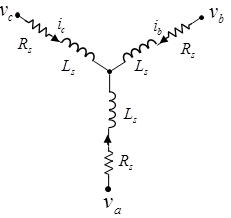
\includegraphics[width=0.3\linewidth]{pmsm_abc.png}
    \caption{Wye Connected PMSM Equivalent Circuit Model}
    \label{fig:pmsm_abc}
\end{figure}

Applying Kirchhoff's voltage law from each phase terminal to the motor
neutral point gives the phase-voltage equations of the PMSM. Note that the motor neutral point is selected as the voltage reference, such that $v_n=0$.

\begin{equation}
\begin{gathered}
\begin{bmatrix}
\label{abc-kvl}
v_a \\
v_b \\
v_c
\end{bmatrix}
=
\begin{bmatrix}
R_s & 0 & 0 \\
0 & R_s & 0 \\
0 & 0 & R_s
\end{bmatrix}
\begin{bmatrix}
i_a \\
i_b \\
i_c
\end{bmatrix}
+
\frac{d}{dt}
\begin{bmatrix}
\lambda_a \\
\lambda_b \\
\lambda_c
\end{bmatrix}
\\[10pt]
\text{or } \quad \mathbf{v}_{abc} = \mathbf{R}_s\mathbf{i}_{abc} + \frac{d\boldsymbol{\lambda}_{abc}}{dt}
\end{gathered}
\end{equation}

Where $R_s$ denotes the stator resistance, and $\lambda_{abc}$ denotes the flux linking each winding. The permanent magnet and the three windings contribute to the total flux linking each winding. The total flux is:

\begin{equation}
\label{eqn2}
\begin{gathered}
\begin{bmatrix}
\lambda_a \\
\lambda_b \\
\lambda_c
\end{bmatrix}
=
\begin{bmatrix}
L_{aa} & L_{ab} & L_{ac} \\
L_{ba} & L_{bb} & L_{bc} \\
L_{ca} & L_{cb} & L_{cc}
\end{bmatrix}
\begin{bmatrix}
i_a \\
i_b \\
i_c
\end{bmatrix}
+
\begin{bmatrix}
\lambda_{am} \\
\lambda_{bm} \\
\lambda_{cm}
\end{bmatrix}
\\[10pt]
\text{or } \quad \boldsymbol{\lambda}_{abc} = \mathbf{L}_{abc}\mathbf{i}_{abc} + \boldsymbol{\lambda}_{m,abc}
\end{gathered}
\end{equation}

Where $L_{aa}$, $L_{bb}$ and $L_{cc}$ are the self inductance's of the stator windings, $L_{ab}$, $L_{ac}$, $L_{ba}$ and so on, are the mutual inductance's of the stator windings, and $\lambda_a$, $\lambda_b$ and $\lambda_c$ are the permanent magnet fluxes linking the stator windings. 

\begin{figure}[H]
    \centering
    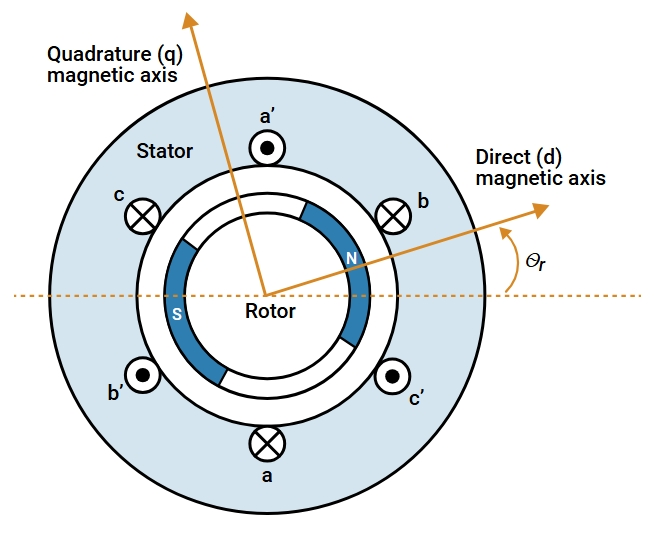
\includegraphics[width=0.45\linewidth]{pmsm_diagram.jpeg}
    \caption{Surface Permanent Magnet Synchronous Motor}
    \label{fig:pmsm_diagram}
\end{figure}


%=========================================================================%
\subsubsection{Flux Linkages}
\paragraph{Winding Inductances}
\label{sec:winding-inductances}
%=========================================================================%


The stator flux linkage introduced in Equation \ref{eqn2} depends on the currents flowing through all three stator phases. Neglecting the permanent-magnet contribution for the moment, the flux linkage produced by the stator currents can be written as:

\begin{equation}
\begin{bmatrix}
\label{winding-inductance-matrix}
\lambda_{as} \\
\lambda_{bs} \\
\lambda_{cs}
\end{bmatrix}
=
\begin{bmatrix}
L_{aa} & L_{ab} & L_{ac} \\
L_{ba} & L_{bb} & L_{bc} \\
L_{ca} & L_{cb} & L_{cc}
\end{bmatrix}
\begin{bmatrix}
i_a \\
i_b \\
i_c
\end{bmatrix}
\end{equation}

or, more compactly,

\begin{equation}
\boldsymbol{\lambda}_{s,abc}
=
\mathbf{L}_{abc}\mathbf{i}_{abc}.
\end{equation}

The diagonal terms of $\mathbf{L}_{abc}$ are the self-inductances of the stator phases, while the off-diagonal terms are the mutual inductances between phases. For example, $L_{aa}$ describes the flux linkage of phase $a$ produced by current $i_a$, whereas $L_{ab}$ describes the flux linkage of phase $a$ produced by current $i_b$.

In general, the inductance relating current in phase $k$ to flux linkage in phase $j$ is defined as

\begin{equation}
    L_{jk} = \frac{\partial \lambda_{js}}{\partial i_k}
\end{equation}

Therefore, in order to determine the elements of the stator inductance matrix, an expression for the magnetic field and resulting flux linkage produced by the stator currents must first be developed. We define the following assumptions:

\begin{enumerate}
    \item \textbf{Constant Air-Gap:} The machine is assumed to be non-salient. The air gap is therefore constant.
    \item \textbf{Angle Invariant Permeability:} The permeability of rare earth magnets is approximately equal to that of air ($\mu_r\approx1.05$), therefore the reluctance is assumed to be invariant to rotor angle.
    \item \textbf{Linear Magnetic Circuit:} The stator and rotor iron cores are assumed to have infinite permeability ($\mu_{Fe} \to \infty$) and operate in the linear region (no magnetic saturation). The entire reluctance of the magnetic circuit is contained within the air gap.
    \item \textbf{No Leakage:} The leakage flux is assumed to be negligible. Therefore no leakage inductance terms exist.
\end{enumerate}

Then, let the air gap be defined as the difference between the rotor and stator radii:

\begin{equation}
    g = r_s - r_r
\end{equation}

Ampere's Law states that:

\begin{equation}
    \oint_C \mathbf{H} \cdot d\mathbf{l} = I_{enc}
\end{equation}

For the contour which lies in the cross section of the PMSM that contains some section of the air gap, stator yoke and rotor, the closed loop line integral of the magnetic field intensity in the air-gap, $\textbf{H}$, is:

\begin{equation}
    \oint_C \mathbf{H} \cdot d\mathbf{l} = \int_{\text{Leg 1}} \mathbf{H} \cdot d\mathbf{l} + \int_{\text{Leg 2}} \mathbf{H} \cdot d\mathbf{l} + \int_{\text{Leg 3}} \mathbf{H} \cdot d\mathbf{l} + \int_{\text{Leg 4}} \mathbf{H} \cdot d\mathbf{l} = i_{\text{enc}}
\end{equation}

Where Leg 1 is the radial path from $r_r^-$ to $r_s^+$, Leg 2 is the arc from $\theta$ to $\theta + \pi$ at radius $r_s^+$, Leg 3 is the radial path from $r_s^+$ to $r_r^-$, and Leg 4 is the arc from $\theta + \pi$ to $\theta$ at radius $r_r^-$. Since we assume the air-gap to be small ($g << r$), we neglect the radial dependence of $\mathbf{r}$ on $\mathbf{H}$. 

\begin{equation}
    \int_{r_r^-}^{r_s^+} H_g(\theta) \, dr + \int_{\text{stator}} \mathbf{H}_{\text{Fe}} \cdot d\mathbf{l} + \int_{r_s^+}^{r_r^-} H_g(\theta + \pi) \, dr + \int_{\text{rotor}} \mathbf{H}_{\text{Fe}} \cdot d\mathbf{l} = i_{\text{enc}}
\end{equation}

Assuming the core iron has near-infinite permeability ($\mu_{\text{Fe}} \to \infty$), the magnetic field intensity required to drive flux through the stator and rotor back-iron is negligible ($\mathbf{H}_{\text{Fe}} \approx \mathbf{0}$). Thus, the line integrals along Leg 2 and Leg 4 evaluate to zero:

\begin{equation}
    H_g(\theta)(r_s^+ - r_r^-) + 0 - H_g(\theta + \pi)(r_r^- - r_s^+) + 0 = i_{\text{enc}}(\theta)
\end{equation}

\begin{equation}
\label{eqn10}
    H_g(\theta) - H_g(\theta + \pi) = \frac{i_{\text{enc}}(\theta)}{g}
\end{equation}

Because the machine is completely symmetrical (both physically and magnetically), the magnetic field entering the rotor at $\theta$ must be equal and opposite to the field leaving it at $\theta + \pi$. Therefore:

\begin{equation}
    H_g(\theta + \pi) = -H_g(\theta)    
\end{equation}

and, from Equation \ref{eqn10}:

\begin{equation}
    H_g(\theta) = \frac{i_{enc}(\theta)}{2g}
\end{equation}

Since the air-gap permeability is assumed equal to that of air, $\mathbf{B} = \mu_0\mathbf{H}$ and:

\begin{equation}
\label{eqn12}
    B_g(\theta) = \frac{\mu_0}{2g}i_{enc}(\theta)
\end{equation}

Because we have assumed the air gap, $g$, to be small relative to the stator radius, we assume the magnetic field crosses the gap purely in the radial direction. That is:

\begin{equation}
    \mathbf{B} = B_g(\theta)\mathbf{\hat{r}}
\end{equation}

The term $i_{enc}(\theta)$ represents the total net current enclosed by our contour from each phase contribution. This depends entirely on how the conductors are distributed in the stator slots. Let $n_a(\theta)$ be the turns density function (conductors per radian) for phase $a$. We define $n_b(\theta)$ and $n_c(\theta)$ similarly. Ampere-Maxewell's Law states that:

\begin{equation}
\label{amp-max-law}
    \iint_{\partial S} \mathbf{J} \cdot d\mathbf{S} = I_{enc}
\end{equation}

Where the total current density, $\mathbf{J}$, is the sum of current density contributions from each phase:

\begin{equation}
    \mathbf{J} = \mathbf{J_a} + \mathbf{J_b} + \mathbf{J_c}
\end{equation}

Using the conductor turns density function, it follows from Equation \ref{amp-max-law} that when a current flows through phases $a$, $b$ and $c$, the total current enclosed by our contour (spanning from $\theta$ to $\theta + \pi$) is:

\begin{equation}
    i_{enc}(\theta) = i_{enc,a}(\theta) + i_{enc,b}(\theta) + i_{enc,c}(\theta)
\end{equation}

\begin{equation}
    i_{enc}(\theta) = i_a\int_{\theta}^{\theta + \pi}{n_a(\theta) \, d\alpha} + i_b\int_{\theta}^{\theta + \pi}{n_b(\theta) \, d\alpha} + i_c\int_{\theta}^{\theta + \pi}{n_c(\theta) \, d\alpha}
\end{equation}

Where $\mathbf{J_n} = i_n n_n(\theta)$ [A/rad]. If we define a winding function specific to each phase, $N_n(\theta)$, as exactly half of its enclosed current contribution, representing the effective turns that contribute to the MMF drop across a single air-gap:

\begin{equation}
    N_a(\theta) = \frac{1}{2} \int_{\theta}^{\theta + \pi} n_a(\alpha) \, d\alpha, \qquad
    N_b(\theta) = \frac{1}{2} \int_{\theta}^{\theta + \pi} n_b(\alpha) \, d\alpha, \qquad
    N_c(\theta) = \frac{1}{2} \int_{\theta}^{\theta + \pi} n_c(\alpha) \, d\alpha
\end{equation}

Then:

\begin{equation}
\label{eqn21}
    i_{enc}(\theta) = 2[N_a(\theta)i_a + N_b(\theta)i_b + N_c(\theta)i_c]
\end{equation}

And, from Equation \ref{eqn12} and Equation \ref{eqn21}:

\begin{equation}
\label{eqn17}
    B_g(\theta) = \frac{\mu_0}{g}[N_a(\theta)i_a + N_b(\theta)i_b + N_c(\theta)i_c]
\end{equation}

Finally, to derive an equation for the total flux linking the stator coil of phase $a$, we use the following relations:

\begin{equation}
\label{flux-eqn}
    \lambda_{as} = \int N_a(\theta) B_g(\theta)\mathbf{\hat{r}} \cdot d\mathbf{A}
\end{equation}

Substituting Equation Equation \ref{eqn17}, we have:

\begin{equation}
    \lambda_{as} = \int_{0}^{2\pi} N_a(\theta)\frac{\mu_0}{g}[N_a(\theta)i_a + N_b(\theta)i_b + N_c(\theta)i_c] r l \, d\theta
\end{equation}

Where $r$ is the effective radius of the air gap, and $l$ is the length of the machine. Factoring out the constants and expanding, we have:

\begin{equation}
    \lambda_{as} = \frac{\mu_0 r l}{g} \left[ i_a\int_{0}^{2\pi} N_a^2(\theta) \, d\theta + i_b\int_{0}^{2\pi} N_a(\theta) N_b(\theta) \, d\theta + i_c\int_{0}^{2\pi} N_a(\theta) N_c(\theta) \, d\theta \right]
\end{equation}

Which is equivalent to:

\begin{equation}
    \lambda_{as} = \lambda_{aa} + \lambda_{ab} + \lambda_{ac}
\end{equation}

\begin{equation}
    \lambda_{as} = L_{aa} i_a + L_{ab} i_b + L_{ac} i_c
\end{equation}

Where at last, the self and mutual inductances, $L_{aa}$, $L_{ab}$ and $L_{ac}$, are defined as:

\begin{equation}
    L_{aa} = \frac{\mu_0 r l}{g} \int_{0}^{2\pi} N_a^2(\theta) \, d\theta
\end{equation}

\begin{equation}
    L_{ab} = \frac{\mu_0 r l}{g} \int_{0}^{2\pi} N_a(\theta) N_b(\theta) \, d\theta
\end{equation}

\begin{equation}
    L_{ac} = \frac{\mu_0 r l}{g} \int_{0}^{2\pi} N_a(\theta) N_c(\theta) \, d\theta
\end{equation}

Repeating for the remaining phases, we find that, in general:

\begin{equation}
\label{self-inductange-general}
    L_{jj} = \frac{\mu_0 r l}{g} \int_{0}^{2\pi} N_j^2(\theta) \, d\theta
\end{equation}

\begin{equation}
\label{mutual-inductance-general}
    L_{jk} = \frac{\mu_0 r l}{g} \int_{0}^{2\pi} N_j(\theta) N_k(\theta) \, d\theta
\end{equation}

Where for the self inductance, $j = k$, as in Equation \ref{self-inductange-general}, and for mutual inductance, $j \neq k$, as in Equation \ref{mutual-inductance-general}.

For a balanced three-phase machine, the three stator windings have identical geometries and differ only by their spatial displacement. If the spatial coordinate $\theta$ is defined as an electrical angle, then phases $b$ and $c$ are shifted from phase $a$ by $120^\circ$ and $240^\circ$, respectively. Therefore, their conductor-density functions may be written as

\begin{equation}
    n_b(\alpha) = n_a\left(\alpha - \frac{2\pi}{3}\right), \qquad
    n_c(\alpha) = n_a\left(\alpha + \frac{2\pi}{3}\right)
\end{equation}

Since the winding function is defined directly from the conductor-density function, the same spatial shifts carry over to the winding functions:

\begin{equation}
    N_b(\theta) = N_a\left(\theta - \frac{2\pi}{3}\right), \qquad
    N_c(\theta) = N_a\left(\theta + \frac{2\pi}{3}\right)
\end{equation}

Thus, each phase has the same winding-function shape, simply shifted around the stator.

From Equation \ref{self-inductange-general}, the self-inductance of any phase is proportional to the integral of the square of its winding function over the full circumference of the machine. Because the three winding functions differ only by a spatial shift, and because the integration spans a complete $2\pi$ period, shifting the winding function does not change the value of the integral. For example,

\begin{equation}
\int_0^{2\pi} N_a^2\left(\theta-\frac{2\pi}{3}\right)\,d\theta = \int_0^{2\pi} N_a^2(\theta)\,d\theta.
\end{equation}

Therefore, all three self-inductances are equal:

\begin{equation}
    L_s = L_{aa} = L_{bb} = L_{cc}
\end{equation}

The same reasoning applies to the mutual inductances. In general:

\begin{equation}
    L_{jk} = \frac{\mu_0 r l}{g} \int_0^{2\pi} N_j(\theta)N_k(\theta)\,d\theta
\end{equation}

The value of this integral depends only on the relative spatial displacement between the two windings. In a balanced three-phase machine, each pair of phases has the same relative displacement of $120^\circ$ electrical, up to sign and periodicity. Consequently, all of the mutual inductances are equal:

\begin{equation}
    L_m = L_{ab} = L_{bc} = L_{ca} = L_{ba} = L_{cb} = L_{ac}
\end{equation}

Finally, the expressions for both self and mutual inductance contain only the stator winding functions and constant geometric parameters. Since the machine is assumed to be non-salient, the effective air gap $g$ does not vary with rotor position. The winding functions are fixed to the stator and therefore also do not depend on the rotor electrical angle $\theta_e$. As a result, the inductances contain no rotor-position dependence:

\begin{equation}
    \frac{\partial L_{jk}}{\partial \theta_e} = 0
\end{equation}

Therefore, for the balanced, non-salient machine considered here, the three self-inductances are equal, the six mutual inductances are equal, and all of them are constant with respect to rotor position.

The preceding expressions are valid for an arbitrary stator winding distribution described by the winding functions $N_a(\theta)$,$N_b(\theta)$, and $N_c(\theta)$. To obtain closed-form expressions for the self and mutual inductances, the stator windings are now assumed to be sinusoidally distributed. Under this assumption, the fundamental
winding functions may be written as:

\begin{equation}
    N_a(\theta) = N_p \cos(\theta)
\end{equation}

\begin{equation}
    N_b(\theta) = N_p \cos\left(\theta-\frac{2\pi}{3}\right)
\end{equation}

\begin{equation}
    N_c(\theta) = N_p \cos\left(\theta+\frac{2\pi}{3}\right)
\end{equation}

where $N_p$ is the peak value of the winding function. Substituting the sinusoidal phase $a$ winding function into the general
self inductance expression, Equation \ref{self-inductange-general}, gives:

\begin{align}
    L_{aa} &= \frac{\mu_0 r l}{g} \int_0^{2\pi} N_p^2 \cos^2(\theta)\,d\theta \\[10pt]
    &= \frac{\mu_0 r l N_p^2}{g} \int_0^{2\pi} \cos^2(\theta)\,d\theta
\end{align}

Since:

\begin{equation}
    \int_0^{2\pi}\cos^2(\theta)\,d\theta = \pi
\end{equation}

the magnetizing component of the phase self inductance is:

\begin{equation}
\label{self-inductance-distributed}
    L_{aa} = \frac{\pi \mu_0 r l N_p^2}{g}
\end{equation}

Similarly, the mutual inductance between phases $a$ and $b$ is:

\begin{align}
    L_{ab} &= \frac{\mu_0 r l}{g} \int_0^{2\pi} N_a(\theta)N_b(\theta)\,d\theta \\[10pt]
    &= \frac{\mu_0 r l N_p^2}{g} \int_0^{2\pi} \cos(\theta) \cos\left(\theta-\frac{2\pi}{3}\right)d\theta
\end{align}

Using:

\begin{equation}
    \int_0^{2\pi} \cos(\theta)\cos(\theta-\phi)\,d\theta = \pi\cos(\phi)
\end{equation}

Gives:

\begin{align}
\label{mutual-inductance-distributued}
    L_{ab} &= \frac{\pi\mu_0 r l N_p^2}{g} \cos\left(\frac{2\pi}{3}\right) \\
    &= -\frac{1}{2} \frac{\pi\mu_0 r l N_p^2}{g}
\end{align}

From Equations \ref{self-inductance-distributed} and \ref{mutual-inductance-distributued}, we can see that:

\begin{equation}
    L_{ab} = -\frac{1}{2}L_{aa}
\end{equation}

Or

\begin{equation}
    L_m = -\frac{1}{2}L_{s}
\end{equation}

Where the negative sign indicates that a positive current, $i_b$, generates a flux that links phase $a$, opposite to phase $a$'s positive flux direction. Then, Equation \ref{winding-inductance-matrix} becomes:

\begin{equation}
\mathbf{L}_{abc}
=
\begin{bmatrix}
L_s & L_m & L_m \\
L_m & L_s & L_m \\
L_m & L_m & L_s
\end{bmatrix}.
\end{equation}


%=========================================================================%
\paragraph{Permanent Magnet Flux Linkage}
\label{pm-flux-linakge}

The permanent magnets contribute an additional component to the total stator flux linkage. Unlike the stator-current-produced flux linkage, the permanent-magnet flux is produced by the rotor and therefore varies with rotor position relative to the stationary stator windings. The permanent-magnet contribution may be written as

\begin{equation}
\boldsymbol{\lambda}_{m,abc}
=
\begin{bmatrix}
\lambda_{am} \\
\lambda_{bm} \\
\lambda_{cm}
\end{bmatrix}
\end{equation}

such that the total stator flux linkage is

\begin{equation}
\boldsymbol{\lambda}_{abc}
=
\mathbf{L}_{abc}\mathbf{i}_{abc}
+
\boldsymbol{\lambda}_{m,abc}
\end{equation}

Each element of $\boldsymbol{\lambda}_{m,abc}$ represents the flux linkage of a stator phase produced by the rotor permanent magnets. To examine the rotor flux, we consider the scenario where the stator currents are zero:

\begin{equation}
    i_a = i_b = i_c = 0
\end{equation}

Because the rotor magnetic field rotates relative to the stator, the permanent-magnet flux linkage depends on rotor position. Similarly to Equation \ref{flux-eqn}, for phase $j$, it may be written generally as:

\begin{equation}
\lambda_{jm}
=
rl
\int_0^{2\pi}
N_j(\theta)\,
B_m(\theta,\theta_e)
\,d\theta
\end{equation}

where $N_j(\theta)$ is the winding function of phase $j$ and $B_m(\theta,\theta_e)$ is the radial air-gap flux density produced by the permanent magnets. Thus, the permanent-magnet flux linkage is determined by the spatial overlap between the rotor magnetic field and the corresponding stator winding. For an ideal, sinusoidal PMSM, $B_m$ is described by:

\begin{equation}
    B_m(\theta, \theta_e) = B_{p}\cos(\theta - \theta_e)
\end{equation}

And $N_j(\theta)$, as described in Section \ref{sec:winding-inductances} using distributed windings, is defined by:

\begin{equation}
    N_a(\theta) = N_p \cos(\theta)
\end{equation}

\begin{equation}
    N_b(\theta) = N_p \cos\left(\theta-\frac{2\pi}{3}\right)
\end{equation}

\begin{equation}
    N_c(\theta) = N_p \cos\left(\theta+\frac{2\pi}{3}\right)
\end{equation}

We can calculate $\lambda_{a,m}$ as:

\begin{equation}
    \lambda_{am} = rlN_p B_{p} \int_0^{2\pi} \cos(\theta)\cos(\theta-\theta_e)\,d\theta
\end{equation}

Using the identity:

\begin{equation}
    \int_0^{2\pi} \cos(\theta)\cos(\theta-\alpha)\,d\theta = \pi\cos(\alpha),
\end{equation}

We obtain:

\begin{equation}
    \lambda_{am} = \lambda_m\cos(\theta_e)
\end{equation}

Where:

\begin{equation}
    \lambda_m = \pi r l N_p B_p
\end{equation}

Is the peak permanent-magnet flux linkage of one phase. Because the stator phases are displaced by $120^\circ$ electrical:

\begin{equation}
    \lambda_{bm} = \lambda_m \cos\left(\theta_e-\frac{2\pi}{3}\right)
\end{equation}

And:

\begin{equation}
    \lambda_{cm} = \lambda_m \cos\left(\theta_e+\frac{2\pi}{3}\right)
\end{equation}

Therefore, the permanent-magnet flux-linkage vector is

\begin{equation}
\boldsymbol{\lambda}_{m,abc}
=
\lambda_m
\begin{bmatrix}
\cos(\theta_e) \\[4pt]
\cos\left(\theta_e-\frac{2\pi}{3}\right) \\[4pt]
\cos\left(\theta_e+\frac{2\pi}{3}\right)
\end{bmatrix}
\end{equation}

This expression describes the permanent-magnet flux linkage of an ideal sinusoidal PMSM.


%=========================================================================%
\paragraph{Summary}

For the balanced, non-salient machine considered here, the stator inductances may be expressed generally in terms of the winding functions. The self-inductance of phase $j$ and mutual inductance between phases $j$ and $k$ are:

\begin{equation}
    L_{jj} = \frac{\mu_0 r l}{g} \int_0^{2\pi} N_j^2(\theta)\,d\theta
\end{equation}

and

\begin{equation}
    L_{jk} = \frac{\mu_0 r l}{g} \int_0^{2\pi} N_j(\theta)N_k(\theta)\,d\theta, \qquad j \neq k
\end{equation}

Assuming sinusoidally distributed stator windings:

\begin{equation}
    N_a(\theta)=N_p\cos(\theta)
\end{equation}

with phases $b$ and $c$ displaced by $\pm 2\pi/3$ electrical, the integrals may be evaluated analytically. Neglecting leakage flux, the self inductances are:

\begin{equation}
    L_{aa}=L_{bb}=L_{cc} = \frac{\pi\mu_0 r l N_p^2}{g} \equiv L_s
\end{equation}

while the mutual inductances are:

\begin{equation}
    L_{ab}=L_{ac}=L_{ba}=L_{bc}=L_{ca}=L_{cb} = -\frac{1}{2}L_s \equiv L_m
\end{equation}

Thus:

\begin{equation}
    L_m = -\frac{1}{2}L_s
\end{equation}

and the stator inductance matrix becomes:

\begin{equation}
\mathbf{L}_{abc}
=
\begin{bmatrix}
L_s & L_m & L_m \\
L_m & L_s & L_m \\
L_m & L_m & L_s
\end{bmatrix}
\end{equation}

For the permanent magnets, assuming a sinusoidal rotor air-gap flux density, the peak permanent-magnet flux linkage of one phase is:

\begin{equation}
    \lambda_m = \pi r l N_p B_m
\end{equation}

The permanent-magnet flux-linkage vector is therefore:

\begin{equation}
\boldsymbol{\lambda}_{m,abc}
=
\lambda_m
\begin{bmatrix}
\cos(\theta_e) \\[4pt]
\cos\left(\theta_e-\frac{2\pi}{3}\right) \\[4pt]
\cos\left(\theta_e+\frac{2\pi}{3}\right)
\end{bmatrix}
\end{equation}

Combining the stator-current-produced and permanent-magnet flux linkages gives the total stator flux-linkage vector from Equation \ref{eqn2}:

\begin{equation}
    \boldsymbol{\lambda}_{abc} = \mathbf{L}_{abc}\mathbf{i}_{abc} + \boldsymbol{\lambda}_{m,abc}
\end{equation}

%=========================================================================%
\subsubsection{Back-EMF}
%=========================================================================%

Recall Equation \ref{abc-kvl} and \ref{eqn2} from Section \ref{equivalent-circuit-model}:

\begin{equation}
\label{eqn80}
    \mathbf{v}_{abc} = \mathbf{R}_s\mathbf{i}_{abc} + \frac{d\boldsymbol{\lambda}_{abc}}{dt}
\end{equation}

\begin{equation}
\label{eqn81}
    \boldsymbol{\lambda}_{abc} = \mathbf{L}_{abc}\mathbf{i}_{abc} + \boldsymbol{\lambda}_{m,abc}
\end{equation}

Combining these equations yields:

\begin{equation}
    \mathbf{v}_{abc} = \mathbf{R}_s\mathbf{i}_{abc} + \frac{d}{dt} \left( \mathbf{L}_{abc}\mathbf{i}_{abc} + \boldsymbol{\lambda}_{m,abc} \right)
\end{equation}

In Section \ref{sec:winding-inductances}, we saw how for a non-salient machine, the winding inductance becomes independent of rotor angle. Specifically:

\begin{equation}
    \frac{\partial \boldsymbol{L}_{abc}}{\partial \theta_e} = 0
\end{equation}

Thus, it follows that:

\begin{equation}
    \frac{d\boldsymbol{L}_{abc}}{dt} = 0
\end{equation}

Therefore:

\begin{equation}
    \mathbf{v}_{abc} = \mathbf{R}_s\mathbf{i}_{abc} + \mathbf{L}_{abc}\frac{d\mathbf{i}_{abc}}{dt} + \frac{d\boldsymbol{\lambda}_{m,abc}}{dt}
\end{equation}

From Section \ref{pm-flux-linakge}, we know the rotor flux, $\boldsymbol{\lambda}_{m,abc}$ as:

\begin{equation}
    \boldsymbol{\lambda}_{m,abc} = \lambda_m
    \begin{bmatrix}
        \cos(\theta_e) \\[4pt]
        \cos\left(\theta_e-\frac{2\pi}{3}\right) \\[4pt]
        \cos\left(\theta_e+\frac{2\pi}{3}\right)
    \end{bmatrix}
\end{equation}

Evaluating the derivative with respect to time, using the chain rule:

\begin{equation}
    \frac{d}{dt} \left[ \lambda_{m}cos(\theta_e) \right] = -\lambda_m sin(\theta_e) \cdot \frac{d\theta_e}{dt}
\end{equation}

\begin{equation}
    \frac{d}{dt} \left[ \lambda_{m}cos(\theta_e - \frac{2\pi}{3}) \right] = -\lambda_m sin(\theta_e - \frac{2\pi}{3}) \cdot \frac{d\theta_e}{dt}
\end{equation}

\begin{equation}
    \frac{d}{dt} \left[ \lambda_{m}cos(\theta_e + \frac{2\pi}{3}) \right] = -\lambda_m sin(\theta_e + \frac{2\pi}{3}) \cdot \frac{d\theta_e}{dt}
\end{equation}

Notice that the derivative of electrical rotor angle is simply the electrical spatial velocity:

\begin{equation}
    \frac{d\theta_e}{dt} = \omega_e
\end{equation}

Recall that $\theta_e$ is the rotor electrical angle, meaning that one cycle is the physical angle rotated when a static magnetic field is applied to the state, and the rotor spins from north to south and back to north. Thus, the conversion between mechanical and electrical angle is proportional to the number of pole pairs in the machine. Specifically:

\begin{equation}
    \theta_e = p\theta_m
\end{equation}

Alternatively:

\begin{equation}
    \omega_e = p\omega_m
\end{equation}

The derivative of the permanent magnet flux linkage with the stator windings is then:

\begin{equation}
    \boldsymbol{e}_{abc} = -\omega_e\lambda_m
    \begin{bmatrix}
        \sin(\theta_e) \\[4pt]
        \sin\left(\theta_e-\frac{2\pi}{3}\right) \\[4pt]
        \sin\left(\theta_e+\frac{2\pi}{3}\right)
    \end{bmatrix}
\end{equation}

Where $\mathbf{e}_{abc}$ is known as the back-EMF. This term is the result of the rotor permanent magnet flux inducing a voltage back into the stator windings.


%=========================================================================%
\subsubsection{PMSM Equations in \texorpdfstring{$abc$}{abc} Frame}
\paragraph{Summary}
%=========================================================================%


Thus, in ABC frame, the equations describing the electrical behavior of a non-salient, PMSM are as follows: 

\begin{equation}
    \mathbf{v}_{abc} = \mathbf{R}_s\mathbf{i}_{abc} + \mathbf{L}_{abc}\frac{d\mathbf{i}_{abc}}{dt} + \boldsymbol{e}_{abc}
\end{equation}

In matrix form:

\begin{equation}
\begin{bmatrix}
v_a \\
v_b \\
v_c
\end{bmatrix}
=
\begin{bmatrix}
R_s & 0 & 0 \\
0 & R_s & 0 \\
0 & 0 & R_s
\end{bmatrix}
\begin{bmatrix}
i_a \\
i_b \\
i_c
\end{bmatrix}
+
\begin{bmatrix}
L_s & L_m & L_m \\
L_m & L_s & L_m \\
L_m & L_m & L_s
\end{bmatrix}
\frac{d}{dt}
\begin{bmatrix}
i_a \\
i_b \\
i_c
\end{bmatrix}
+
\begin{bmatrix}
e_a \\
e_b \\
e_c
\end{bmatrix}
\end{equation}

Where $R_s$ is the stator winding phase resistance, $L_s$ is the phase self inductance,

\begin{equation}
    L_{s} = \frac{\pi \mu_0 r l N_p^2}{g}
\end{equation}

Where $r$ is the effective air gap radius, $l$ is the length of the machine, $N_p$ is the peak amplitude of the spatial winding function, and $g$, is the air gap. $L_m$ is the mutual inductance between phases,

\begin{equation}
    L_m = -\frac{1}{2}L_s
\end{equation}

$\mathbf{e}_{abc}$ is the back-EMF vector,

\begin{equation}
    \boldsymbol{e}_{abc} = -\omega_e\lambda_m
    \begin{bmatrix}
        \sin(\theta_e) \\[4pt]
        \sin\left(\theta_e-\frac{2\pi}{3}\right) \\[4pt]
        \sin\left(\theta_e+\frac{2\pi}{3}\right)
    \end{bmatrix}
\end{equation}

Where $\lambda_m$ is the peak amplitude of the permanent magnet flux linkage,

\begin{equation}
    \lambda_m = \pi r l N_p B_m
\end{equation}

Where $B_m$ is the peak amplitude of the permanent magnet flux density inherent to its material and geometric properties. $\theta_e$ is the electrical rotor angle,

\begin{equation}
    \theta_{e,r} = p\theta_{m,r}
\end{equation}


%=========================================================================%
\subsection{\texorpdfstring{$\alpha\beta$}{Alpha-Beta} Frame}
\label{sec:alpha-beta-frame}
%=========================================================================%

The preceding model describes the PMSM directly in terms of the three physical stator phases. Before introducing the $\alpha\beta$ frame, it is useful to distinguish a physical vector from the coordinates used to represent it. We will later see how the primary benefit of the transformation to $\alpha\beta$ frame is the compression of a balanced three dimensional quantity to a two dimensional quantity. First, we examine the transform in 3D. 

A vector may exist independently of any particular coordinate system. Once a basis is selected, the vector may be represented by a set of scalar coordinates describing its components along each basis direction. For a three phase quantity, $\mathbf{f}$, let:

\begin{equation}
    \mathbf{B}_{abc} = \{ \mathbf{\hat{e}}_{a}, \mathbf{\hat{e}}_{b}, \mathbf{\hat{e}}_{c} \}
\end{equation}

Denote the $abc$ basis vectors. An arbitrary vector may then be written as:

\begin{equation}
    \mathbf{f} = f_a \mathbf{\hat{e}}_{a} + f_b \mathbf{\hat{e}}_{b} + f_c \mathbf{\hat{e}}_{c}
\end{equation}

With coordinates:

\begin{equation}
    \mathbf{f}_{abc} =
    \begin{bmatrix}
        f_a \\[1pt]
        f_b \\[1pt]
        f_c
    \end{bmatrix}
\end{equation}

The three phase quantities are independent coordinate directions and may therefore be represented by the orthonormal basis:

\begin{equation}
    \mathbf{\hat{e}}_a =
    \begin{bmatrix}
        1 \\[1pt]
        0 \\[1pt]
        0
    \end{bmatrix}, 
    \qquad
    \mathbf{\hat{e}}_b =
    \begin{bmatrix}
        0 \\[1pt]
        1 \\[1pt]
        0 \\[1pt]
    \end{bmatrix},
    \qquad
    \mathbf{\hat{e}}_c =
    \begin{bmatrix}
        0 \\[1pt]
        0 \\[1pt]
        1 \\[1pt]
    \end{bmatrix}
\end{equation}

Thus, the phase variable space is fundamentally three dimensional. For a balanced, wye connected PMSM, an isolated neutral imposes that:

\begin{equation}
\label{sum-of-currents-zero}
    i_a + i_b + i_c = 0
\end{equation}

As a result, although the phase variable space is three dimensional, the allowable stator currents have only two linearly independent dimensions, since one current can be specified in terms of the other two. Hence only a 2D plane is required to specify the stator currents. This yields the typical $abc$ frame phasor diagram in Figure \ref{fig:abc-phasors}. 

\begin{figure}[H]
    \centering
    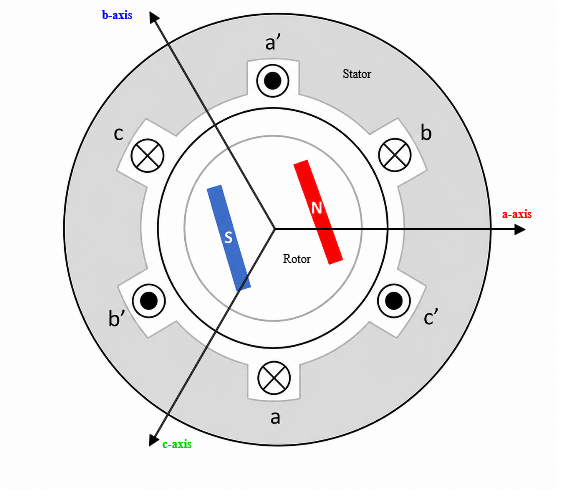
\includegraphics[width=0.5\linewidth]{abc-phasors.png}
    \caption{$abc$ Frame Phasor Diagram}
    \label{fig:abc-phasors}
\end{figure}

Within the three dimensional space, recall that Equation \ref{sum-of-currents-zero} is the equation for a plane, which can be seen in Figure \ref{fig:abc-balanced-plane}

\begin{figure}[H]
    \centering
    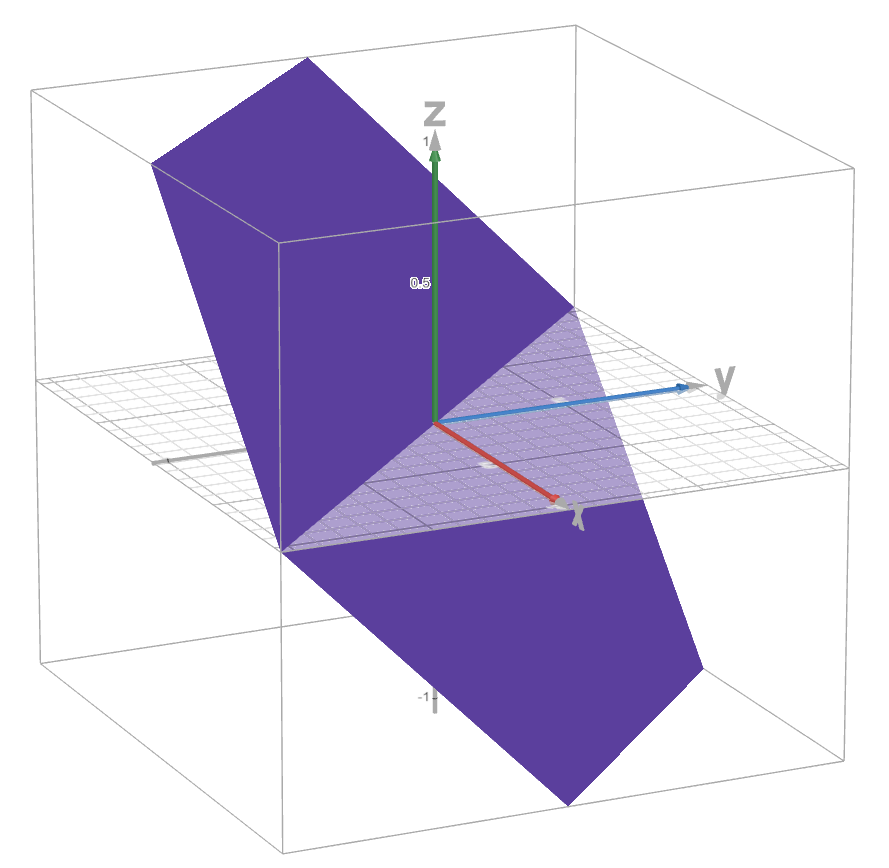
\includegraphics[width=0.5\linewidth]{abc-balanced-plane.png}
    \caption{$abc$ Axis and Balanced Plane}
    \label{fig:abc-balanced-plane}
\end{figure}

It is the projection of the three phase axis onto the balanced plane where the familiar, $120^\circ$ separated diagram originates from:

\begin{figure}[H]
    \centering
    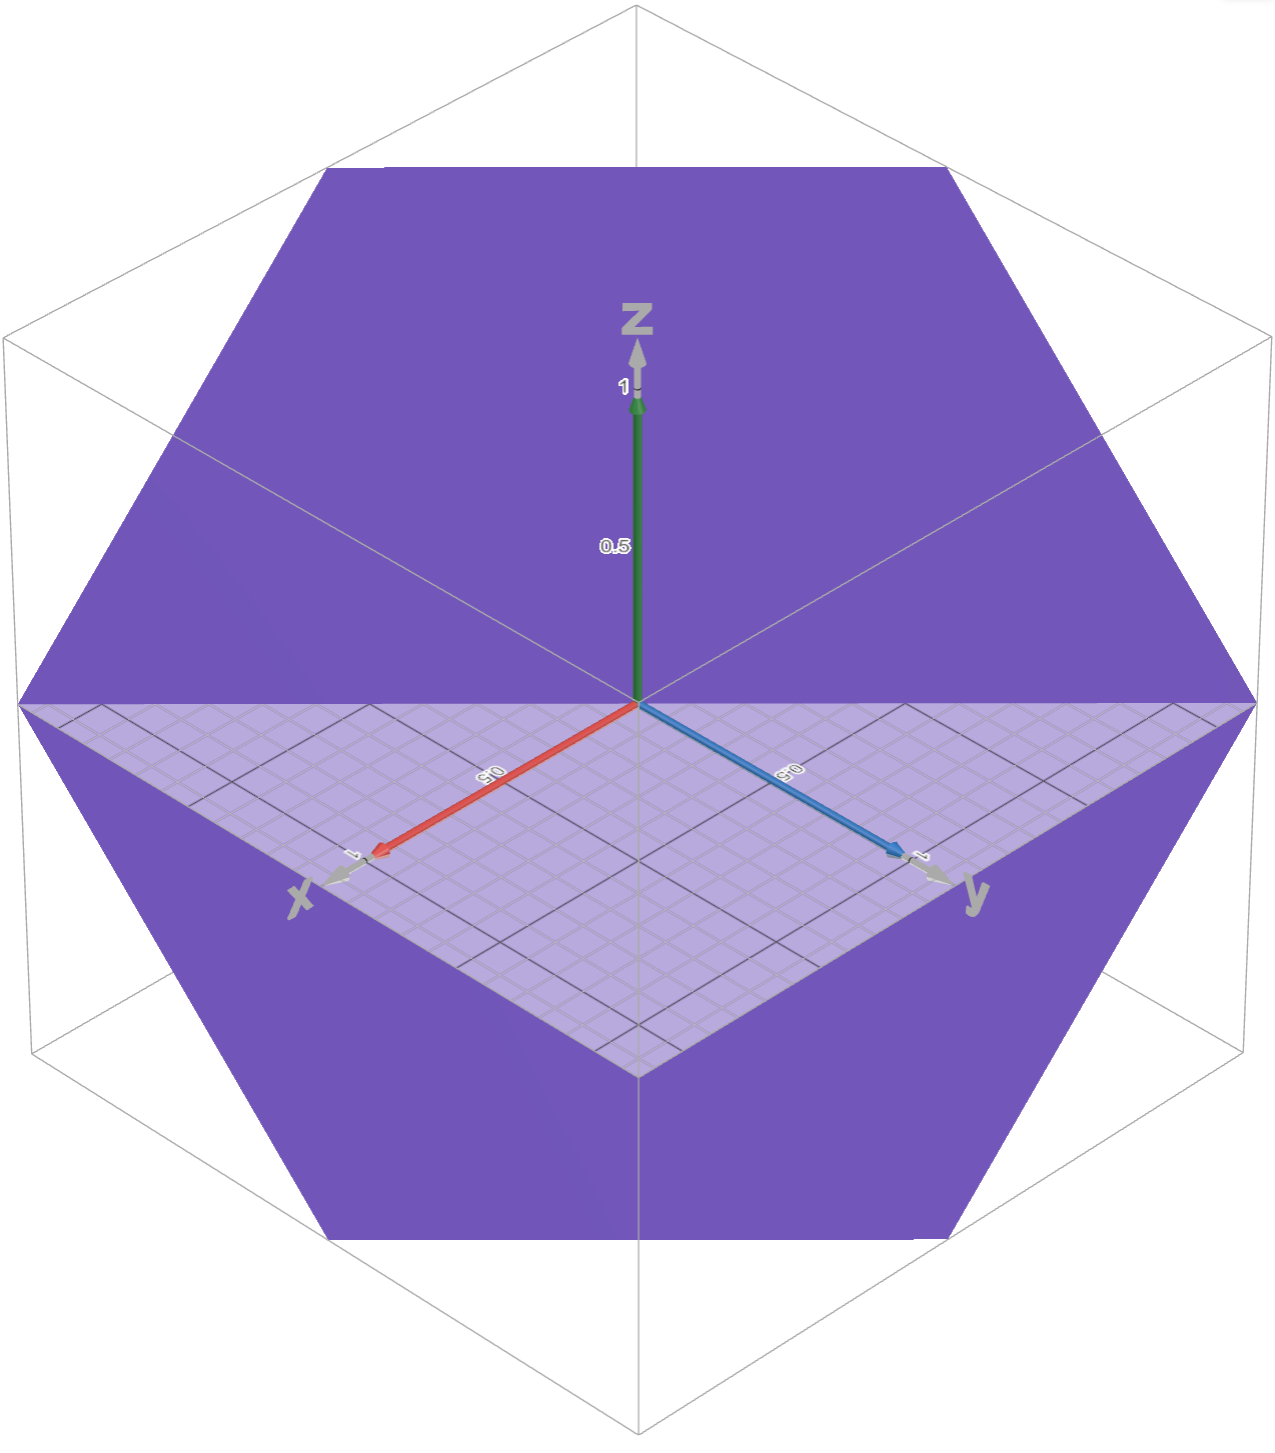
\includegraphics[width=0.5\linewidth]{120projection.png}
    \caption{Projection of $abc$ Frame onto Balanced Plane}
    \label{fig:120projection}
\end{figure}

%=========================================================================%
\subsubsection{Clarke Transformation}
\label{clarke-transformation}

The objective of the Clarke transformation is to construct a coordinate system which is naturally aligned with this two dimensional subspace.

The plane:

\begin{equation}
    f_a + f_b + f_c = 0
\end{equation}

Has the normal vector:

\begin{equation}
    \mathbf{\hat{n}} =
    \begin{bmatrix}
        1 \\
        1 \\
        1
    \end{bmatrix}_{abc}
\end{equation}

Normalizing this vector defines the zero sequence basis direction:

\begin{equation}
    \mathbf{\hat{e}}_0 = \frac{1}{\sqrt{3}}
    \begin{bmatrix}
        1 \\
        1 \\
        1
    \end{bmatrix}_{abc}
\end{equation}

A vector directed entirely along $\mathbf{\hat{e}}_0$ has equal components in each phase, and therefore represents a zero-sequence quantity. The zero sequence axis is perpendicular to the balanced plane, as shown in Figure \ref{fig:zero-sequence-axis}.

\begin{figure}[H]
    \centering
    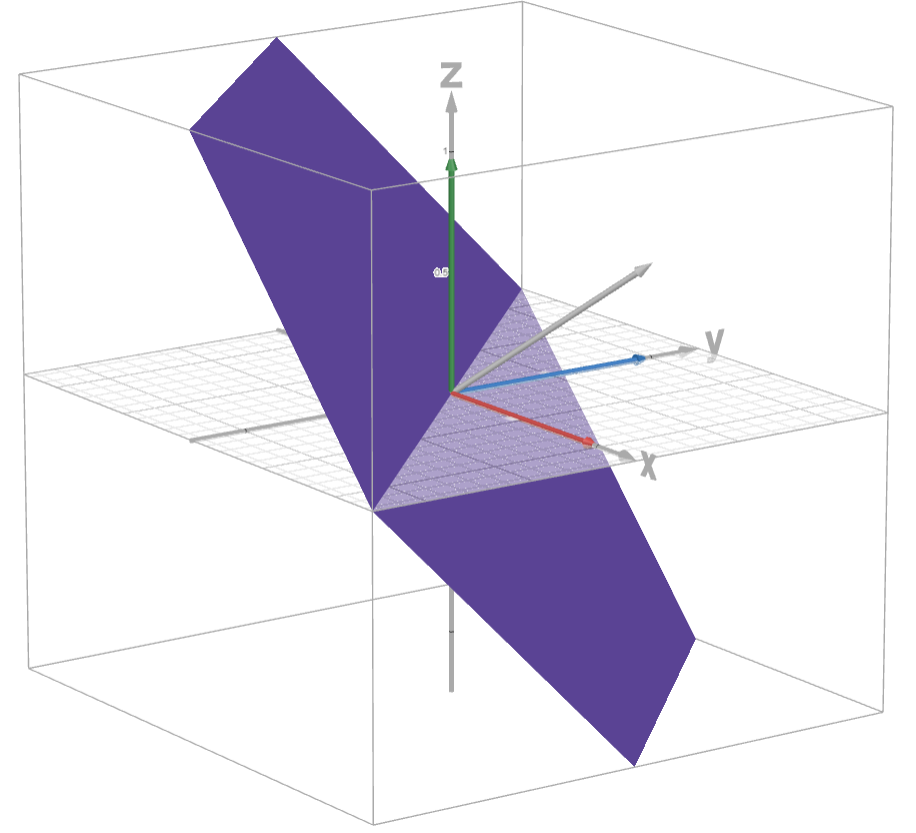
\includegraphics[width=0.5\linewidth]{zerosequence-axis.png}
    \caption{Zero Sequence Axis \& $abc$ Frame}
    \label{fig:zero-sequence-axis}
\end{figure}

An increase in this direction corresponds to an equal increase in all three phases. This can be imagined by sweeping the balanced plane along the zero sequence axis and visualizing the increase or decrease along each of the $abc$ axis.

We then define two additional orthogonal basis vectors within the balanced plane to define the new coordinate system based on the zero-sequence axis, in which balanced phasors can be represented by only two dimensions. These are defined as the $\alpha$ and $\beta$ axes.


%=========================================================================%
\paragraph{Construction of the \texorpdfstring{$\alpha$}{Alpha}-Axis}
%=========================================================================%


The orientation of the perpendicular $\alpha$ and $\beta$ axes is not unique. In favor of simplicity, and by convention, the $\alpha$-axis is chosen to align with the projection of the phase $a$ axis onto the balanced plane. This is equal to the projection of the phase $a$ basis vector onto the zero sequence vector, subtracted from the phase $a$ vector. In other words, the projection of the phase $a$ axis onto the balanced plane is the component of $a$ that lies normal to the balanced plane subtracted from the phase $a$ basis vector. 

\begin{equation}
    \operatorname{proj}_0(\hat{\mathbf e}_a) = \frac{\mathbf{\hat{e}}_a \cdot \mathbf{\hat{e}}_0}{||\mathbf{\hat{e}}_0||^2} \mathbf{\hat{e}}_0
\end{equation}

Since $\mathbf{\hat{e}}_0$ is a unit vector:

\begin{align}
    \operatorname{proj}_0(\hat{\mathbf e}_a)
        &= (\hat{\mathbf e}_a \cdot \hat{\mathbf e}_0)\hat{\mathbf e}_0 \\[4pt]
        &= \left(
        \begin{bmatrix}1\\0\\0\end{bmatrix}
        \cdot
        \frac{1}{\sqrt{3}}
        \begin{bmatrix}1\\1\\1\end{bmatrix}
        \right)\hat{\mathbf e}_0 \\[4pt]
        &= \frac{1}{\sqrt{3}}\hat{\mathbf e}_0 \\[4pt]
        &= \frac{1}{3}
        \begin{bmatrix}1\\1\\1\end{bmatrix}
\end{align}

Then, the component of $\mathbf{\hat{e}}_a$ that lies in the balanced plane is:

\begin{align}
    \mathbf{\hat{e}}_{a0} &= \mathbf{\hat{e}}_a - \operatorname{proj}_0(\hat{\mathbf e}_a) \\[4pt]
    &=
    \begin{bmatrix}
        1 \\
        0 \\
        0
    \end{bmatrix}
    - \frac{1}{3}
    \begin{bmatrix}
        1 \\
        1 \\
        1
    \end{bmatrix} \\[4pt]
    \mathbf{\hat{e}}_{a0} &=
    \begin{bmatrix}
        \frac{2}{3} \\
        -\frac{1}{3} \\
        -\frac{1}{3}
    \end{bmatrix}
\end{align}

Notice that:

\begin{equation}
    \frac{2}{3} - \frac{1}{3} - \frac{1}{3} = 0
\end{equation}

Confirming this vector lies in the balanced plane. Normalizing this vector, we select it as the $\alpha$-axis:

\begin{equation}
    \mathbf{\hat{e}}_\alpha = \frac{1}{\sqrt{6}}
    \begin{bmatrix}
        2 \\
        -1 \\
        -1
    \end{bmatrix}
\end{equation}

We show this in the following figure, where $\mathbf{\hat{e}}_a$ is shown in red along the x-axis, $\mathbf{\hat{e}}_b$ is shown in blue along the y-axis, $\mathbf{\hat{e}}_c$ is shown in green along the z-axis, the zero-sequence vector, $\mathbf{\hat{e}}_0$, is shown in gray perpendicular to the balanced plane in purple, the projection of $\mathbf{\hat{e}}_a$ onto the zero-sequence vector is shown in orange, and $\alpha$-axis is shown in blue in the balanced plane. 

Note that even in this depiction where phase $a$ lies on the left, phase $b$ lies on the right and phase $c$ points upwards, which differs from the conventional illustration with phase $a$ at $0^\circ$ and so on, the fundamental mathematics do not change.  

\begin{figure}[H]
    \centering
    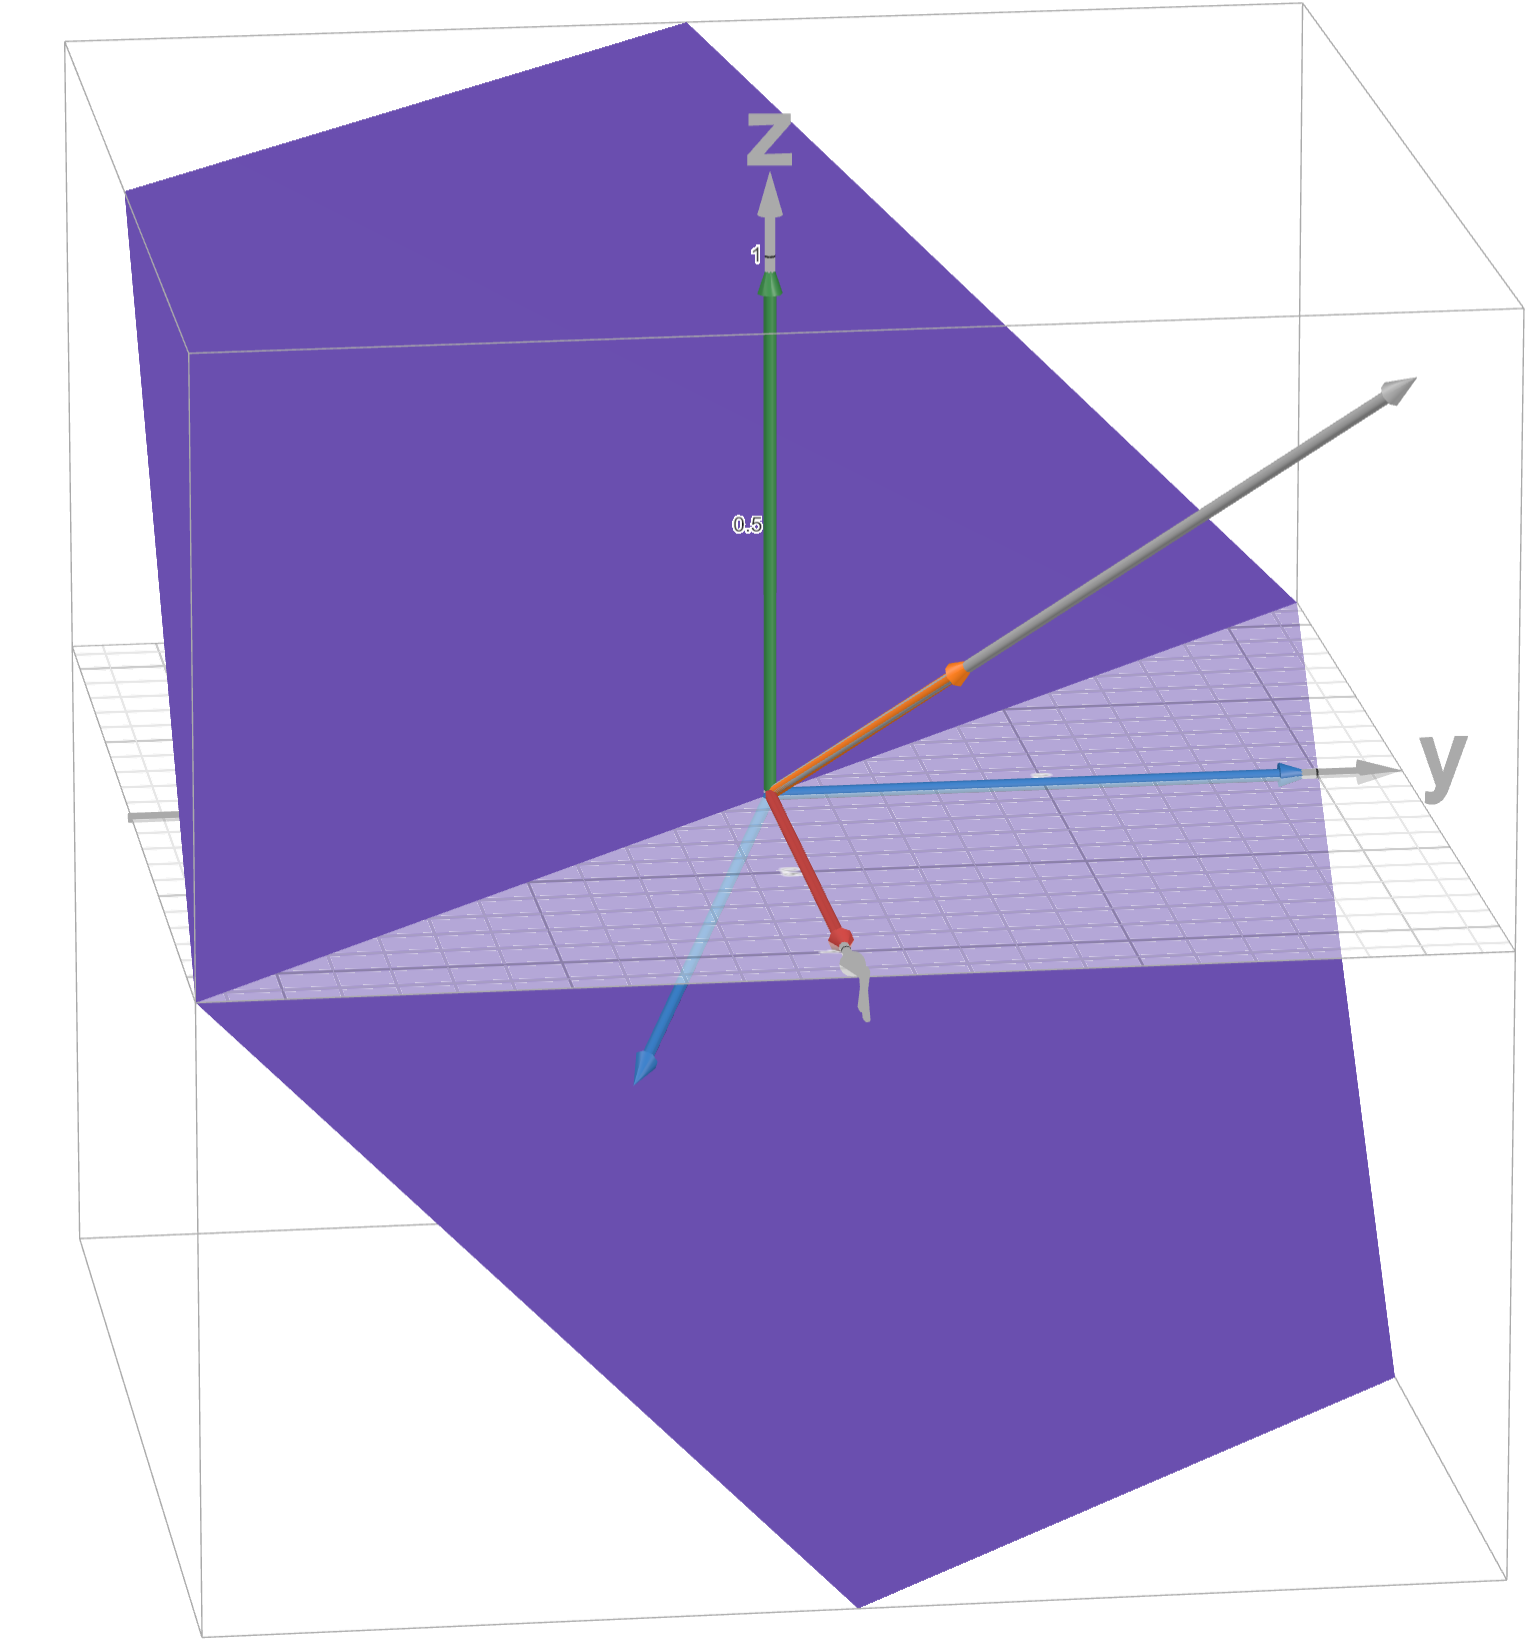
\includegraphics[width=0.5\linewidth]{projection.png}
    \caption{$abc$ Basis Vectors, Zero-Sequence Vector, $\operatorname{proj}_0(\hat{\mathbf e}_a)$, and the Projection of $\mathbf{\hat{e}}_a$} onto the Balanced Plane
    \label{fig:projection}
\end{figure}


%=========================================================================%
\paragraph{Construction of the \texorpdfstring{$\beta$}{Beta}-Axis}

The remaining basis vector must lie within the balanced plane and be perpendicular to both $\mathbf{\hat{e}}_a$ and $\mathbf{\hat{e}}_0$. Choosing ($\alpha$, $\beta$, $0$) to form a right handed coordinate system:

\begin{equation}
    \mathbf{\hat{e}}_\beta = \mathbf{\hat{e}}_0 \times \mathbf{\hat{e}}_\alpha
\end{equation}

Thus:

\begin{equation}
    \mathbf{\hat{e}}_\beta = \frac{1}{\sqrt{2}}
    \begin{bmatrix}
        0 \\
        1 \\
        -1
    \end{bmatrix}
\end{equation}

The $\alpha\beta0$ frame as seen from the $abc$ frame can be seen in Figure \ref{fig:alphabeta-abc} where the $abc$ axes are in red, blue and green respectively, and $\alpha\beta0$ can be seen in orange, gray and purple, respectively. 

\begin{figure}
    \centering
    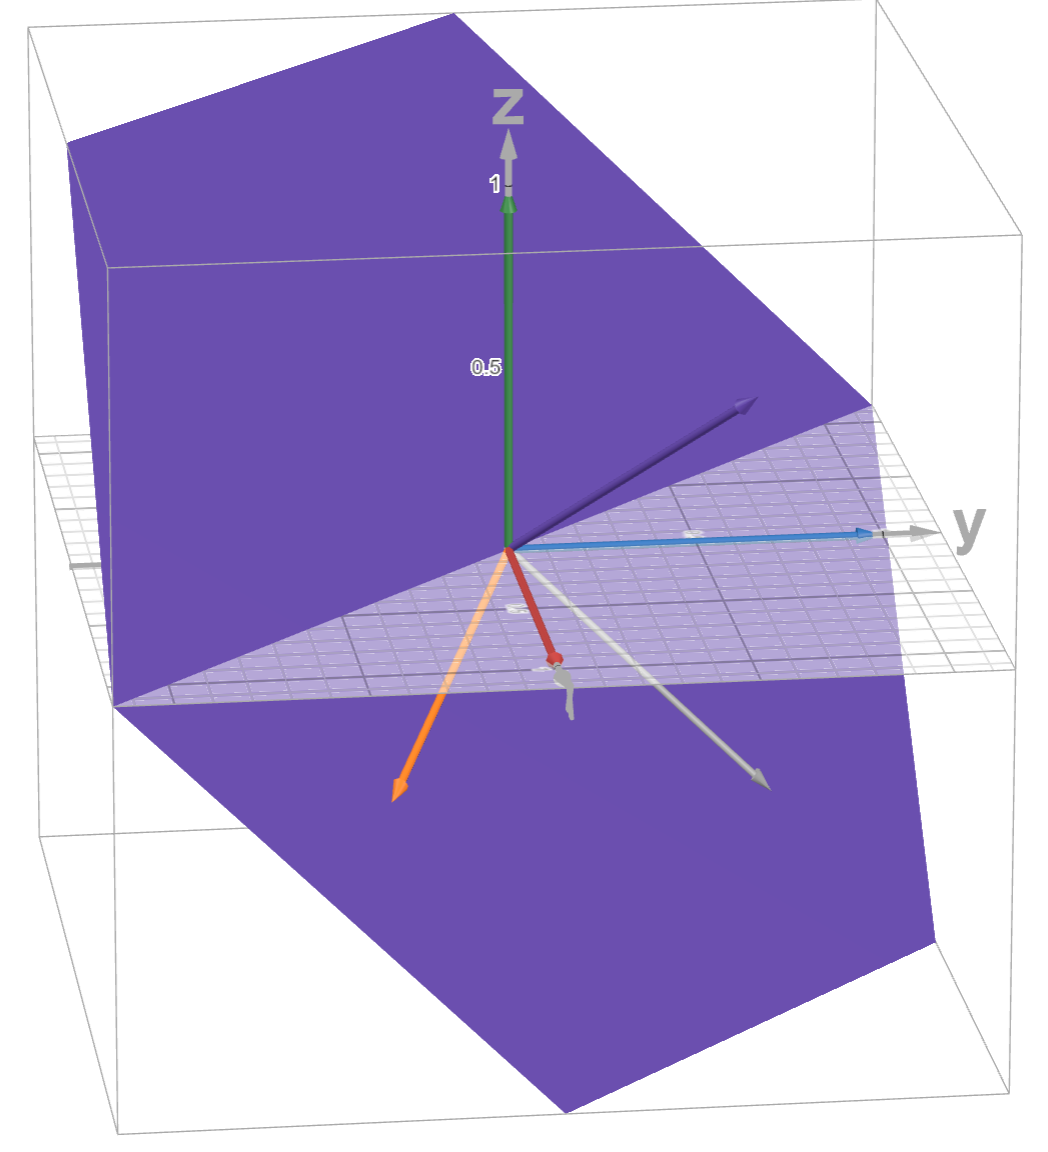
\includegraphics[width=0.5\linewidth]{alphabeta_abc.png}
    \caption{$\alpha\beta0$ Frame as seen from the $abc$ Reference Frame}
    \label{fig:alphabeta-abc}
\end{figure}

Combining the basis vectors to form the transformation matrix from $\alpha\beta0$ to $abc$, we find that:

\begin{equation}
    \mathbf{P}
    =
    \begin{bmatrix}
        \sqrt{\frac{2}{3}} & 0 & \frac{1}{\sqrt{3}} \\[2mm]
        -\frac{1}{\sqrt{6}} & \frac{1}{\sqrt{2}} & \frac{1}{\sqrt{3}} \\[2mm]
        -\frac{1}{\sqrt{6}} & -\frac{1}{\sqrt{2}} & \frac{1}{\sqrt{3}}
    \end{bmatrix}
\end{equation}

Factoring out $\sqrt{\frac{2}{3}}$:

\begin{equation}
    \mathbf{P}
    =
    \sqrt{\frac{2}{3}}
    \begin{bmatrix}
        1 & 0 & \frac{1}{\sqrt{2}} \\[2mm]
        -\frac{1}{2} & \frac{\sqrt{3}}{2} & \frac{1}{\sqrt{2}} \\[2mm]
        -\frac{1}{2} & -\frac{\sqrt{3}}{2} & \frac{1}{\sqrt{2}}
    \end{bmatrix}
\end{equation}

Therefore:

\begin{equation}
    \mathbf{f}_{abc} = \mathbf{P}\mathbf{f}_{\alpha\beta0}
\end{equation}


%=========================================================================%
\paragraph{Power-Invariant Clarke Transformation}
The result we seek is the transform from $abc$ frame to $\alpha\beta0$ frame. Specially, we require:

\begin{equation}
    \mathbf{f}_{\alpha\beta0} = \mathbf{P}^{-1} \mathbf{f}_{abc}
\end{equation}

Rather than calculate the matrix inverse explicitly (which would also produce the correct result regardless), since we have specifically constructed $\mathbf{\hat{e}}_\alpha$, $\mathbf{\hat{e}}_\beta$ and $\mathbf{\hat{e}}_0$ to be orthogonal unit vectors:

\begin{equation}
    P^TP = I
\end{equation}

Compare this with the definition of the inverse:

\begin{equation}
    P^{-1}P = I
\end{equation}

Therefore:

\begin{equation}
    P^{-1} = P^T
\end{equation}

And finally, we define the forward, power invariant Clarke transform as:

\begin{equation}
    \mathbf{T}_{c,p} = \mathbf{P}^{T}
    =
    \sqrt{\frac{2}{3}}
    \begin{bmatrix}
        1 & -\frac{1}{2} & -\frac{1}{2} \\[2mm]
        0 & \frac{\sqrt{3}}{2} & -\frac{\sqrt{3}}{2} \\[2mm]
        \frac{1}{\sqrt{2}} & \frac{1}{\sqrt{2}} & \frac{1}{\sqrt{2}}
    \end{bmatrix}
\end{equation}

Thus the transform from $abc$ frame to $\alpha\beta0$ frame is:

\begin{equation}
    \begin{bmatrix}
        f_{\alpha} \\
        f_{\beta} \\
        f_{0}
    \end{bmatrix}
    =
    \sqrt{\frac{2}{3}}
    \begin{bmatrix}
        1 & -\frac{1}{2} & -\frac{1}{2} \\[2mm]
        0 & \frac{\sqrt{3}}{2} & -\frac{\sqrt{3}}{2} \\[2mm]
        \frac{1}{\sqrt{2}} & \frac{1}{\sqrt{2}} & \frac{1}{\sqrt{2}}
    \end{bmatrix}
    \begin{bmatrix}
        f_a \\
        f_b \\
        f_c
    \end{bmatrix}
\end{equation}

Or:

\begin{equation}
    \mathbf{f}_{\alpha\beta0} = \mathbf{T}_{c,p} \mathbf{f}_{abc}
\end{equation}

With the inverse as:

\begin{equation}
    \begin{bmatrix}
        f_a \\
        f_b \\
        f_c
    \end{bmatrix}
    =
    \sqrt{\frac{2}{3}}
    \begin{bmatrix}
        1 & 0 & \frac{1}{\sqrt{2}} \\[2mm]
        -\frac{1}{2} & \frac{\sqrt{3}}{2} & \frac{1}{\sqrt{2}} \\[2mm]
        -\frac{1}{2} & -\frac{\sqrt{3}}{2} & \frac{1}{\sqrt{2}}
    \end{bmatrix}
    \begin{bmatrix}
        f_{\alpha} \\
        f_{\beta} \\
        f_0
    \end{bmatrix}
\end{equation}

Or:

\begin{equation}
    \mathbf{f}_{abc} = \mathbf{T}_{c,p}^{-1} \mathbf{f}_{\alpha\beta0}
\end{equation}

Where: 

\begin{equation}
    \mathbf{T}_{c,p}^{-1}
    =
    \sqrt{\frac{2}{3}}
    \begin{bmatrix}
        1 & 0 & \frac{1}{\sqrt{2}} \\[2mm]
        -\frac{1}{2} & \frac{\sqrt{3}}{2} & \frac{1}{\sqrt{2}} \\[2mm]
        -\frac{1}{2} & -\frac{\sqrt{3}}{2} & \frac{1}{\sqrt{2}}
    \end{bmatrix}
\end{equation}

and:

\begin{equation}
    \mathbf{T}_{c,p}^{-1} = \mathbf{T}_{c,p}^T
\end{equation}

The transformation derived above is referred to as the power invariant Clarke transformation. Since the $\alpha$, $\beta$ and zero-sequence axes were constructed as an orthogonal basis, the resulting transformation is orthogonal and therefore preserves the dot product between vectors. When applied to three phase voltage and current vectors, the dot product is conserved, and therefore:

\begin{equation}
    v_ai_a + v_bi_b + v_ci_c = v_\alpha i_\alpha + v_\beta i_\beta + v_0i_0
\end{equation}

The preservation of power is the origin of the term, \textit{power invariant}. A consequence of this normalization is that the magnitude of a balanced three phase system is not preserved. In control of PMSM's, the amplitude invariant transformation is generally the preferred form since a command of 5V or 5A, should still result in the same 5V/5A after the transformation. This motivates the introduction of the amplitude invariant form discussed shortly.  

Before this, we lastly recall that for a balanced three phase quantity, the instantaneous phase components satisfy:

\begin{equation}
\label{sum0}
    f_a + f_b + f_c = 0
\end{equation}

Consequently, the corresponding vector lies entirely within the plane defined by Equation \ref{sum0}. Since the zero sequence axis is normal to this plane, a balanced three phase vector has no component in the zero sequence direction, and therefore $f_0 = 0$. Hence for a balanced three phase system only, we can disregard the zero sequence component entirely, and the Clarke transformation simplifies to a transformation from 3D to 2D, as shown below:

\begin{equation}
    \begin{bmatrix}
        f_{\alpha} \\
        f_{\beta}
    \end{bmatrix}
    =
    \sqrt{\frac{2}{3}}
    \begin{bmatrix}
        1 & -\frac{1}{2} & -\frac{1}{2} \\[2mm]
        0 & \frac{\sqrt{3}}{2} & -\frac{\sqrt{3}}{2}
    \end{bmatrix}
    \begin{bmatrix}
        f_a \\
        f_b \\
        f_c
    \end{bmatrix}
\end{equation}

Or:

\begin{equation}
    \mathbf{f}_{\alpha\beta}
    =
    \mathbf{T}_{c,p}\mathbf{f}_{abc}
\end{equation}

Where:

\begin{equation}
    \mathbf{T}_{c,p}
    =
    \sqrt{\frac{2}{3}}
    \begin{bmatrix}
        1 & -\frac{1}{2} & -\frac{1}{2} \\[2mm]
        0 & \frac{\sqrt{3}}{2} & -\frac{\sqrt{3}}{2}
    \end{bmatrix}
\end{equation}

The same applies to the inverse:

\begin{equation}
    \begin{bmatrix}
        f_a \\
        f_b \\
        f_c
    \end{bmatrix}
    =
    \sqrt{\frac{2}{3}}
    \begin{bmatrix}
        1 & 0 \\[2mm]
        -\frac{1}{2} & \frac{\sqrt{3}}{2} \\[2mm]
        -\frac{1}{2} & -\frac{\sqrt{3}}{2}
    \end{bmatrix}
    \begin{bmatrix}
        f_{\alpha} \\
        f_{\beta}
    \end{bmatrix}
\end{equation}

Compactly:

\begin{equation}
    \mathbf{f}_{abc}
    =
    \mathbf{T}_{c,p}^{-1}\mathbf{f}_{\alpha\beta}
\end{equation}

Where:

\begin{equation}
    \mathbf{T}_{c,p}^{-1}
    =
    \sqrt{\frac{2}{3}}
    \begin{bmatrix}
        1 & 0 \\[2mm]
        -\frac{1}{2} & \frac{\sqrt{3}}{2} \\[2mm]
        -\frac{1}{2} & -\frac{\sqrt{3}}{2}
    \end{bmatrix}
\end{equation}


%=========================================================================%
\paragraph{Amplitude-Invariant Clarke Transformation}
\label{sec-amp-invar-clarke}
%=========================================================================%

As noted previously, while the power-invariant Clarke transformation preserves inner products and the orthonormality of the coordinate system, it does not preserve the peak amplitude of a balanced three-phase quantity. In particular, consider a balanced three-phase quantity of peak amplitude $F$:

\begin{align}
    f_a &= F\cos(\theta) \\
    f_b &= F\cos\left(\theta-\frac{2\pi}{3}\right) \\
    f_c &= F\cos\left(\theta+\frac{2\pi}{3}\right)
\end{align}

Applying the power-invariant Clarke transformation gives:

\begin{align}
    f_{\alpha,p} &= \sqrt{\frac{3}{2}}F\cos(\theta) \\
    f_{\beta,p}  &= \sqrt{\frac{3}{2}}F\sin(\theta)
\end{align}

The magnitude of the resulting vector is therefore:

\begin{align}
    \left\|\mathbf{f}_{\alpha\beta,P}\right\|
    &= \sqrt{f_{\alpha,P}^{2}+f_{\beta,P}^{2}} \\
    &= \sqrt{\frac{3}{2}}F
    \label{PI-clarke-scaling}
\end{align}

Thus, although the power-invariant transformation preserves the norm of the original three dimensional vector, the magnitude of the resulting rotating $\alpha\beta$ vector is $\sqrt{3/2}$ times the peak amplitude of the individual phase quantities. For control of PMSMs, it is often more convenient for these quantities to have the same amplitude. Deriving the amplitude invariant form begins with the power invariant form:

\begin{equation}
    \begin{bmatrix}
        f_{\alpha} \\
        f_{\beta} \\
        f_{0}
    \end{bmatrix}
    =
    \sqrt{\frac{2}{3}}
    \begin{bmatrix}
        1 & -\frac{1}{2} & -\frac{1}{2} \\[2mm]
        0 & \frac{\sqrt{3}}{2} & -\frac{\sqrt{3}}{2} \\[2mm]
        \frac{1}{\sqrt{2}} & \frac{1}{\sqrt{2}} & \frac{1}{\sqrt{2}}
    \end{bmatrix}
    \begin{bmatrix}
        f_a \\
        f_b \\
        f_c
    \end{bmatrix}
\end{equation}

Expanding the rows:

\begin{align}
    f_{\alpha,p} &= \sqrt{\frac{2}{3}}\left( f_a - \frac{1}{2}f_b - \frac{1}{2}f_c \right) \\[4pt]
    f_{\beta,p} &= \sqrt{\frac{2}{3}}\left( \frac{\sqrt{3}}{2}f_b - \frac{\sqrt{3}}{2}f_c \right) =  \frac{1}{\sqrt{2}}(f_b - f_c)\\[4pt]
    f_{0,p} &= \sqrt{\frac{2}{3}}\frac{1}{\sqrt{2}} \left( f_a + f_b + f_c \right) = \frac{1}{\sqrt{3}}(f_a + f_b + f_c)
\end{align}

For a balanced three-phase quantity, from Equation \ref{PI-clarke-scaling} we know the $\alpha\beta$ vector has a magnitude of $\sqrt{3/2}$. For amplitude invariance, the magnitude of this vector should be $F$. Therefore, to obtain an $\alpha\beta$ vector whose magnitude is equal to the peak phase amplitude $F$, the $\alpha$ and $\beta$ components must be scaled by:

\begin{equation}
    \sqrt{\frac{2}{3}}
\end{equation}

Thus:

\begin{align}
\label{eqn155}
    f_{\alpha,a} &= \sqrt{\frac{2}{3}}f_{\alpha,p} = \frac{2}{3} \left( f_a - \frac{1}{2}f_b - \frac{1}{2}f_c \right) \\[4pt]
    f_{\beta,a} &= \sqrt{\frac{2}{3}}f_{\beta,p} = \frac{1}{\sqrt{3}}(f_b - f_c) = \frac{2}{3}(\frac{\sqrt{3}}{2}f_b - \frac{\sqrt{3}}{2}f_c)
\label{eqn156}
\end{align}

The zero-sequence component requires a different normalization. Consider a three phase set containing only a zero-sequence quantity for which all three components are in phase (recall the zero-sequence basis is the direction in which all three phases change equally):

\begin{equation}
    f_a = f_b = f_c = F
\end{equation}

Under the power-invariant transformation:

\begin{equation}
    f_{0,p} = \frac{1}{\sqrt{3}}(F + F + F) = \sqrt{3}F
\end{equation}

In other words, this vector in $abc$ frame points entirely in the zero-sequence direction. After the power invariant Clarke transformation, its coordinate along $f_{0,p}$ is $\sqrt{3}F$. To preserve the amplitude of a pure zero-sequence quantity, the zero-sequence component must therefore be scaled by $1/\sqrt{3}$:

\begin{align}
    f_{0,a}
    &= \frac{1}{\sqrt{3}}f_{0,p} \\[2mm]
    &= \frac{1}{3}(f_a + f_b + f_c) \\[2mm]
    &= \frac{2}{3}(\frac{1}{2}f_a + \frac{1}{2}f_b + \frac{1}{2}f_c)
\label{eqn161}
\end{align}

From Equations \ref{eqn155}, \ref{eqn156} and \ref{eqn161}, the amplitude-invariant Clarke transformation is therefore:

\begin{equation}
    \begin{bmatrix}
        f_{\alpha} \\
        f_{\beta} \\
        f_0
    \end{bmatrix}
    =
    \frac{2}{3}
    \begin{bmatrix}
        1 & -\frac{1}{2} & -\frac{1}{2} \\[2mm]
        0 & \frac{\sqrt{3}}{2} & -\frac{\sqrt{3}}{2} \\[2mm]
        \frac{1}{2} & \frac{1}{2} & \frac{1}{2}
    \end{bmatrix}
    \begin{bmatrix}
        f_a \\
        f_b \\
        f_c
    \end{bmatrix}
\end{equation}

Or:

\begin{equation}
    \mathbf{f}_{\alpha\beta}
    =
    \mathbf{T}_{c,a}\mathbf{f}_{abc}
\end{equation}

With:

\begin{equation}
    \mathbf{T}_{c,a}
    =
    \frac{2}{3}
    \begin{bmatrix}
        1 & -\frac{1}{2} & -\frac{1}{2} \\[2mm]
        0 & \frac{\sqrt{3}}{2} & -\frac{\sqrt{3}}{2} \\[2mm]
        \frac{1}{2} & \frac{1}{2} & \frac{1}{2}
    \end{bmatrix}
\end{equation}

Then its inverse is:

\begin{equation}
    \begin{bmatrix}
        f_a \\
        f_b \\
        f_c
    \end{bmatrix}
    =
    \begin{bmatrix}
        1 & 0 & 1 \\[2mm]
        -\frac{1}{2} & \frac{\sqrt{3}}{2} & 1 \\[2mm]
        -\frac{1}{2} & -\frac{\sqrt{3}}{2} & 1
    \end{bmatrix}
    \begin{bmatrix}
        f_{\alpha} \\
        f_{\beta} \\
        f_0
    \end{bmatrix}
\end{equation}

Or:

\begin{equation}
    \mathbf{f}_{abc}
    =
    \mathbf{T}_{c,a}^{-1}\mathbf{f}_{\alpha\beta0}
\end{equation}

With:

\begin{equation}
    \mathbf{T}_{c,a}^{-1}
    =
    \begin{bmatrix}
        1 & 0 & 1 \\[2mm]
        -\frac{1}{2} & \frac{\sqrt{3}}{2} & 1 \\[2mm]
        -\frac{1}{2} & -\frac{\sqrt{3}}{2} & 1
    \end{bmatrix}
\end{equation}

Note that unlike the power-invariant transformation, $T_{c,a}^T \neq T_{c,a}^{-1}$. However, like the power-invariant Clarke transform, for a balanced three phase system:

\begin{equation}
    f_a + f_b + f_c = 0
\end{equation}

And the corresponding transformed $\alpha\beta$ frame vector lies entirely in this plane (i.e the zero-sequence component is zero). Hence the Clarke transform can be reduced from a three dimensional transform to two dimensional:

The amplitude-invariant Clarke transformation for a balanced three-phase system is:

\begin{equation}
    \begin{bmatrix}
        f_{\alpha} \\
        f_{\beta}
    \end{bmatrix}
    =
    \frac{2}{3}
    \begin{bmatrix}
        1 & -\frac{1}{2} & -\frac{1}{2} \\
        0 & \frac{\sqrt{3}}{2} & -\frac{\sqrt{3}}{2}
    \end{bmatrix}
    \begin{bmatrix}
        f_a \\
        f_b \\
        f_c
    \end{bmatrix}
\end{equation}

Or:

\begin{equation}
    \mathbf{f}_{\alpha\beta}
    =
    \mathbf{T}_{c,a}\mathbf{f}_{abc}
\end{equation}

with:

\begin{equation}
    \mathbf{T}_{c,a}
    =
    \frac{2}{3}
    \begin{bmatrix}
        1 & -\frac{1}{2} & -\frac{1}{2} \\
        0 & \frac{\sqrt{3}}{2} & -\frac{\sqrt{3}}{2}
    \end{bmatrix}
\end{equation}

Under the balanced-system constraint $f_a+f_b+f_c=0$, the inverse Clarke transformation is:

\begin{equation}
    \begin{bmatrix}
        f_a \\
        f_b \\
        f_c
    \end{bmatrix}
    =
    \begin{bmatrix}
        1 & 0 \\
        -\frac{1}{2} & \frac{\sqrt{3}}{2} \\
        -\frac{1}{2} & -\frac{\sqrt{3}}{2}
    \end{bmatrix}
    \begin{bmatrix}
        f_{\alpha} \\
        f_{\beta}
    \end{bmatrix}
\end{equation}

Or:

\begin{equation}
    \mathbf{f}_{abc} = \mathbf{T}_{c,a}^{-1}\mathbf{f}_{\alpha\beta}
\end{equation}

Where:

\begin{equation}
    \mathbf{T}_{c,a}^{-1}
    =
    \begin{bmatrix}
        1 & 0 \\
        -\frac{1}{2} & \frac{\sqrt{3}}{2} \\
        -\frac{1}{2} & -\frac{\sqrt{3}}{2}
    \end{bmatrix}
\end{equation}

Note that since the reduced Clarke transformation matrix is not square, it does not have a true matrix inverse. However, for a balanced three-phase system, where $f_a+f_b+f_c=0$, the three original phase quantities can still be recovered from $f_\alpha$ and $f_\beta$. For simplicity, we refer to this as the inverse Clarke transform. If we imagine such a definition for the inverse of a non-square matrix does exist, then for the reduced Clark transform only:

\begin{equation}
    \mathbf{T}_{c,a}^{-1} = \frac{3}{2}\mathbf{T}_{c,a}^{T}
\end{equation}

Putting it all together, for an arbitrary three phase quantity, $\mathbf{f}_{abc}$:

\begin{align}
    f_a &= F\cos(\theta) \\
    f_b &= F\cos\left(\theta-\frac{2\pi}{3}\right) \\
    f_c &= F\cos\left(\theta+\frac{2\pi}{3}\right)
\end{align}

The $\alpha\beta$ components become:

\begin{equation}
    \begin{bmatrix}
        f_{\alpha} \\
        f_{\beta} \\
        f_0
    \end{bmatrix}
    =
    \frac{2}{3}
    \begin{bmatrix}
        1 & -\frac{1}{2} & -\frac{1}{2} \\[2mm]
        0 & \frac{\sqrt{3}}{2} & -\frac{\sqrt{3}}{2} \\[2mm]
        \frac{1}{2} & \frac{1}{2} & \frac{1}{2}
    \end{bmatrix}
    \begin{bmatrix}
        f_a \\
        f_b \\
        f_c
    \end{bmatrix}
\end{equation}

Applying the amplitude-invariant Clarke transformation gives:

\begin{equation}
    \begin{bmatrix}
        f_{\alpha} \\
        f_{\beta} \\
        f_0
    \end{bmatrix}
    =
    \begin{bmatrix}
        \frac{2}{3}f_a-\frac{1}{3}f_b-\frac{1}{3}f_c \\
        \frac{1}{\sqrt{3}}f_b-\frac{1}{\sqrt{3}}f_c \\
        \frac{1}{3}f_a+\frac{1}{3}f_b+\frac{1}{3}f_c
    \end{bmatrix}
\end{equation}

Substituting the balanced three-phase quantities:

\begin{align}
    f_{\alpha}
    &=
    \frac{2}{3}F\cos(\theta)
    -\frac{1}{3}F\cos\left(\theta-\frac{2\pi}{3}\right)
    -\frac{1}{3}F\cos\left(\theta+\frac{2\pi}{3}\right) \\[2mm]
    f_{\beta}
    &=
    \frac{1}{\sqrt{3}}F\cos\left(\theta-\frac{2\pi}{3}\right)
    -\frac{1}{\sqrt{3}}F\cos\left(\theta+\frac{2\pi}{3}\right) \\[2mm]
    f_0
    &=
    \frac{1}{3}F\cos(\theta)
    +\frac{1}{3}F\cos\left(\theta-\frac{2\pi}{3}\right)
    +\frac{1}{3}F\cos\left(\theta+\frac{2\pi}{3}\right)
\end{align}

Using the identity $\cos(A-B)+\cos(A+B)=2\cos(A)\cos(B)$:

\begin{align}
    f_{\alpha}
    &=
    \frac{2}{3}F\cos(\theta)
    -\frac{1}{3}F
    \left[
        2\cos(\theta)\cos\left(\frac{2\pi}{3}\right)
    \right] \\[2mm]
    &=
    \frac{2}{3}F\cos(\theta)
    -\frac{2}{3}F\cos(\theta)
    \left(-\frac{1}{2}\right) \\[2mm]
    &=
    F\cos(\theta)
\end{align}

Similarly, using $\cos(A-B)-\cos(A+B)=2\sin(A)\sin(B)$:

\begin{align}
    f_{\beta}
    &=
    \frac{F}{\sqrt{3}}
    \left[
        \cos\left(\theta-\frac{2\pi}{3}\right)
        -
        \cos\left(\theta+\frac{2\pi}{3}\right)
    \right] \\[2mm]
    &=
    \frac{F}{\sqrt{3}}
    \left[
        2\sin(\theta)\sin\left(\frac{2\pi}{3}\right)
    \right] \\[2mm]
    &=
    \frac{F}{\sqrt{3}}
    \left[
        2\sin(\theta)\frac{\sqrt{3}}{2}
    \right] \\[2mm]
    &=
    F\sin(\theta)
\end{align}

For the zero-sequence component:

\begin{align}
    f_0
    &=
    \frac{F}{3}
    \left[
        \cos(\theta)
        +
        \cos\left(\theta-\frac{2\pi}{3}\right)
        +
        \cos\left(\theta+\frac{2\pi}{3}\right)
    \right] \\[2mm]
    &=
    \frac{F}{3}
    \left[
        \cos(\theta)
        +
        2\cos(\theta)\cos\left(\frac{2\pi}{3}\right)
    \right] \\[2mm]
    &=
    \frac{F}{3}
    \left[
        \cos(\theta)-\cos(\theta)
    \right] \\[2mm]
    &=0
\end{align}

Therefore:

\begin{equation}
\label{alpha-beta-0-3p-result}
    \begin{bmatrix}
        f_{\alpha} \\
        f_{\beta} \\
        f_0
    \end{bmatrix}
    =
    \begin{bmatrix}
        F\cos(\theta) \\
        F\sin(\theta) \\
        0
    \end{bmatrix}
\end{equation}

Or, if using the reduced Clarke transform:

\begin{equation}
\label{alpha-beta-3p-result}
    \begin{bmatrix}
        f_{\alpha} \\
        f_{\beta}
    \end{bmatrix}
    =
    \begin{bmatrix}
        F\cos(\theta) \\
        F\sin(\theta)
    \end{bmatrix}
\end{equation}

Notice that a balanced three phase quantity transformed by the Clarke transformation yields a rotating vector in the $\alpha\beta$ plane with constant magnitude. 

%=========================================================================%
\paragraph{Geometric Interpretation}
\label{geometric-interpretation}
%=========================================================================%

We have just seen how the new $\alpha\beta$ axes are derived, where the $\alpha$-axis is chosen to be aligned with the magnetic axis of phase $a$, and the $\beta$-axis is displaced from it by $90^\circ$ electrical. The amplitude-invariant Clarke transformation is shown in 2D in Figure \ref{fig:clarke}.

\begin{figure}[H]
    \centering
    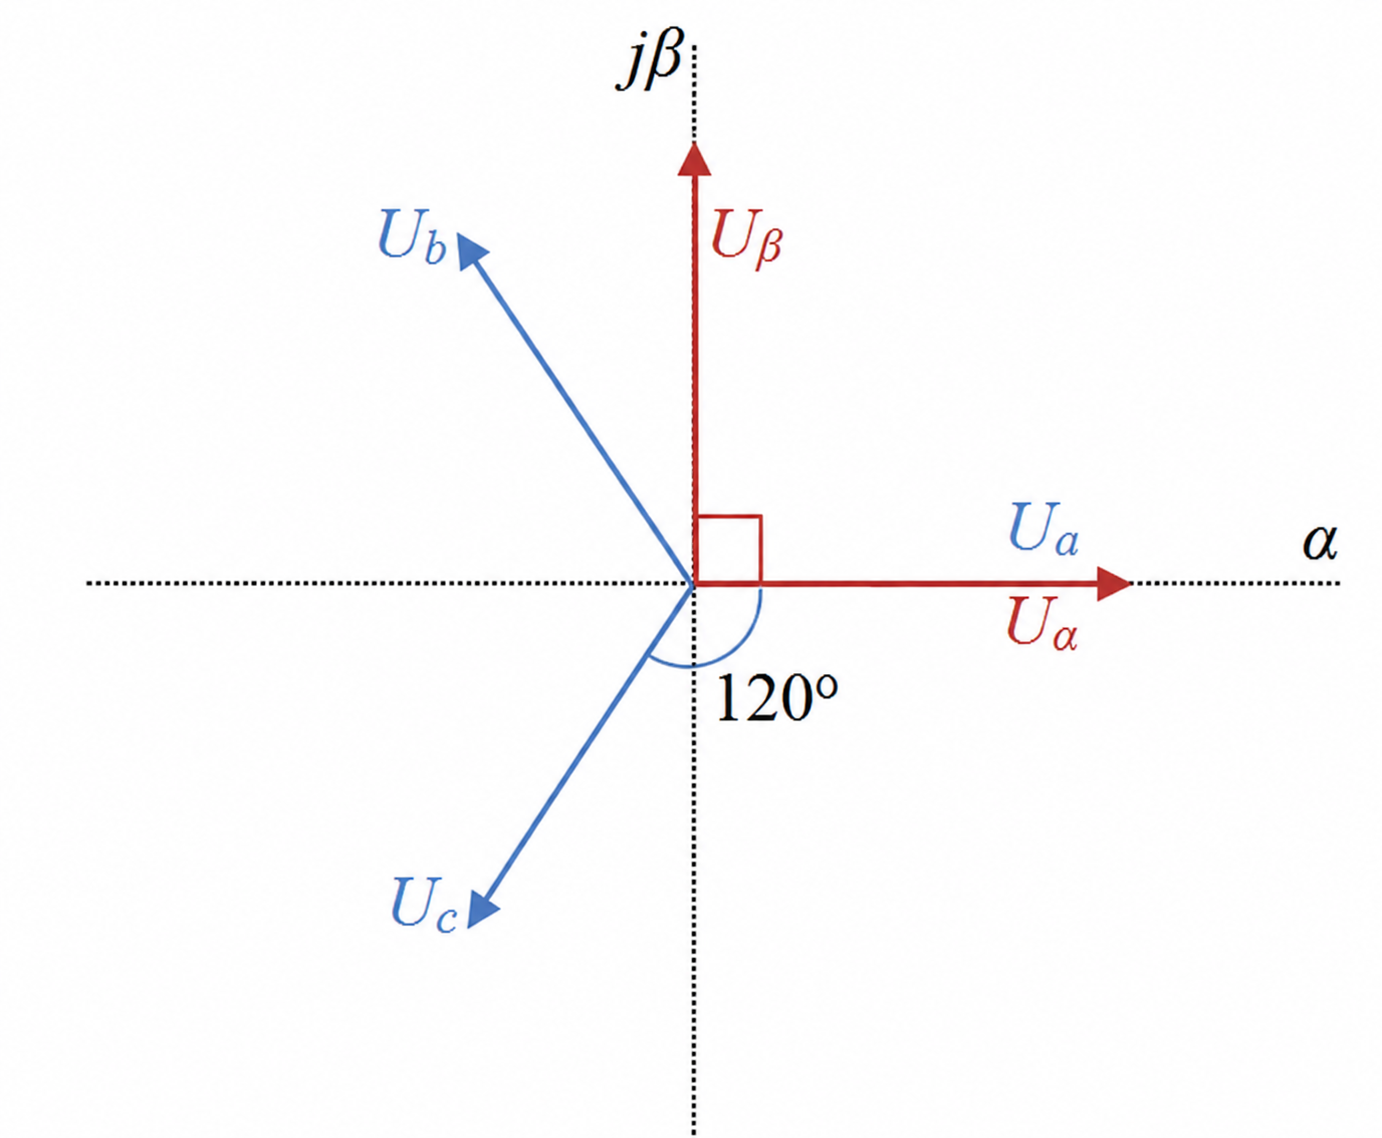
\includegraphics[width=0.4\linewidth]{clarke.png}
    \caption{$abc$ and $\alpha\beta$ Frames}
    \label{fig:clarke}
\end{figure}

The transform fundamentally represents a change of basis from one coordinate system to another. We can understand this geometrically using the rules of linear algebra. To determine the transformation matrix that converts a vector in frame 1 to the same vector in the coordinates of frame 2, we express the basis vectors of frame 1 as seen by frame 2 as column vectors in a matrix.

From Figure \ref{fig:clarke}, we can see that the $a$ and $\alpha$ axis are the same. Hence the $a$ axis as seen by the $\alpha\beta$ frame is simply:

\begin{equation}
    \hat{\mathbf a}
    =
    \begin{bmatrix}
        1 \\
        0
    \end{bmatrix}
\end{equation}

The $b$ axis as seen by the $\alpha\beta$ frame is the vector with length one and $120^\circ$ ($\frac{2\pi}{3}$ rad) of phase:

\begin{equation}
    \hat{\mathbf b}
    =
    \begin{bmatrix}
        \cos\left(\frac{2\pi}{3}\right) \\
        \sin\left(\frac{2\pi}{3}\right)
    \end{bmatrix}
    =
    \begin{bmatrix}
        -\frac{1}{2} \\
        \frac{\sqrt{3}}{2}
    \end{bmatrix}
\end{equation}

Similarly, the $c$ axis as seen by the $\alpha\beta$ frame is the vector with length one and $-120^\circ$ or $240^\circ$ ($-\frac{2\pi}{3}$ or $\frac{4\pi}{3}$ rad) of phase: 

\begin{equation}
    \hat{\mathbf c}
    =
    \begin{bmatrix}
        \cos\left(\frac{4\pi}{3}\right) \\
        \sin\left(\frac{4\pi}{3}\right)
    \end{bmatrix}
    =
    \begin{bmatrix}
        -\frac{1}{2} \\
        -\frac{\sqrt{3}}{2}
    \end{bmatrix}
\end{equation}

The transformation matrix thus has these vectors as columns:

\begin{equation}
\label{clarke-transform-variant}
    \begin{bmatrix}
        f_\alpha \\
        f_\beta
    \end{bmatrix}
    =
    \begin{bmatrix}
        1 & -\frac{1}{2} & -\frac{1}{2} \\
        0 & \frac{\sqrt{3}}{2} & -\frac{\sqrt{3}}{2}
    \end{bmatrix}
    \begin{bmatrix}
        f_a \\
        f_b \\
        f_c
    \end{bmatrix}
\end{equation}

As with before, while Equation \ref{clarke-transform-variant} describes the geometric change of basis between coordinate systems, it introduces a scaling issue. Suppose we again have a 3-phase quantity, $\mathbf{f}_{abc}$:

\begin{equation}
    \begin{gathered}
        f_a = F\cos(\theta) \\[5pt]
        f_b = F\cos(\theta - \frac{2\pi}{3}) \\[5pt]
        f_c = F\cos(\theta + \frac{2\pi}{3})
    \end{gathered}
\end{equation}

Applying the transformation yields:

\begin{equation}
    \begin{bmatrix}
        f_\alpha \\[1pt]
        f_\beta
    \end{bmatrix}
    =
    \begin{bmatrix}
        F\left[\cos(\theta) - \frac{1}{2}\cos(\theta - \frac{2\pi}{3}) - \frac{1}{2}\cos(\theta + \frac{2\pi}{3})\right] \\[1pt]
        F\left[\frac{\sqrt{3}}{2}\cos(\theta - \frac{2\pi}{3}) - \frac{\sqrt{3}}{2}\cos(\theta + \frac{2\pi}{3})\right]
    \end{bmatrix}
\end{equation}

Then using the identities:

\begin{equation}
    \cos(A+B) + \cos(A-B) = 2\cos{A}\cos{B}
\end{equation}

\begin{equation}
    \cos(A-B) - \cos(A+B) = 2\sin{A}\sin{B}
\end{equation}

\begin{equation}
    \begin{bmatrix}
        f_\alpha \\[1pt]
        f_\beta
    \end{bmatrix}
    =
    \begin{bmatrix}
        F\left[\cos(\theta) - \cos(\theta)\cos(\frac{2\pi}{3})\right] \\[1pt]
        F\left[\sqrt{3}\sin(\theta)\sin(\frac{2\pi}{3})\right]
    \end{bmatrix}
\end{equation}

Simplifying:

\begin{equation}
    \begin{bmatrix}
        f_\alpha \\[1pt]
        f_\beta
    \end{bmatrix}
    =
    \begin{bmatrix}
        \frac{3}{2}F\cos(\theta) \\[1pt]
        \frac{3}{2}F\sin(\theta)]
    \end{bmatrix}
\end{equation}

Thus in its current form, the transform introduces an additional factor of $\frac{3}{2}$. For this reason, the Clarke Transform introduces an additional factor of $\frac{2}{3}$ to cancel this out. The balanced Clarke Transform is then:

\begin{equation}
\label{clarke-transform}
    \begin{bmatrix}
        f_\alpha \\
        f_\beta
    \end{bmatrix}
    = \frac{2}{3}
    \begin{bmatrix}
        1 & -\frac{1}{2} & -\frac{1}{2} \\
        0 & \frac{\sqrt{3}}{2} & -\frac{\sqrt{3}}{2}
    \end{bmatrix}
    \begin{bmatrix}
        f_a \\
        f_b \\
        f_c
    \end{bmatrix}
\end{equation}

Where we denote $\mathbf{T}_c$ as:

\begin{equation}
\label{clarke-transform-matrix}
    \mathbf{T}_c =
    \frac{2}{3}
    \begin{bmatrix}
        1 & -\frac{1}{2} & -\frac{1}{2} \\
        0 & \frac{\sqrt{3}}{2} & -\frac{\sqrt{3}}{2}
    \end{bmatrix}
\end{equation}


%=========================================================================%
\subsubsection{PMSM Equations in \texorpdfstring{$\alpha\beta$}{Alpha-Beta} Frame}
%=========================================================================%

Finally, we can convert the synchronous machine $abc$ frame equations to $\alpha\beta$ frame. Note that from here onward, in regards to the forwards Clarke transform, we now exclusively refer to the reduced amplitude invariant form, denoted $\mathbf{T}_c$, unless otherwise specified. Recall the $abc$ frame equations from Section \ref{sec:abc-frame}:

\begin{equation}
\label{abc-eqn}
    \mathbf{v}_{abc} = \mathbf{R}_s\mathbf{i}_{abc} + \mathbf{L}_{abc}\frac{d\mathbf{i}_{abc}}{dt} + \boldsymbol{e}_{abc}
\end{equation}

Where:

\begin{equation}
    \mathbf{L}_{abc} =
    \begin{bmatrix}
        L_s & L_m & L_m \\
        L_m & L_s & L_m \\
        L_m & L_m & L_s
    \end{bmatrix}
\end{equation}

We also know from Section \ref{clarke-transformation} that the Clarke Transform converts vectors in $abc$ frame to $\alpha\beta$ frame:

\begin{equation}
    \mathbf{f}_{\alpha\beta} = \mathbf{T}_c \mathbf{f}_{abc}
\end{equation}

Where $\mathbf{T}_c$ is:

\begin{equation}
    \mathbf{T}_c =
    \frac{2}{3}
    \begin{bmatrix}
        1 & -\frac{1}{2} & -\frac{1}{2} \\
        0 & \frac{\sqrt{3}}{2} & -\frac{\sqrt{3}}{2}
    \end{bmatrix}
\end{equation}

Therefore:

\begin{equation}
    \mathbf{v}_{\alpha\beta} = \mathbf{T}_c \mathbf{v}_{abc}, \qquad
    \mathbf{i}_{\alpha\beta} = \mathbf{T}_c \mathbf{i}_{abc}, \qquad
    \mathbf{e}_{\alpha\beta} = \mathbf{T}_c \mathbf{e}_{abc}
\end{equation}

We will return back to the back-EMF vector shortly. Multiplying Equation \ref{abc-eqn} by the Clarke Transform, we get:

\begin{equation}
    \mathbf{T}_c\mathbf{v}_{abc} = \mathbf{R}_s\mathbf{T}_c\mathbf{i}_{abc} + \mathbf{T}_c\mathbf{L}_{abc}\frac{d\mathbf{i}_{abc}}{dt} + \mathbf{T}_c\boldsymbol{e}_{abc}
\end{equation}

Where since $\mathbf{R}_s$ is scalar, commutativity applies. We can also see that because $\mathbf{T}_c$ is constant, it follows from:

\begin{equation}
    \mathbf{f}_{abc} = \mathbf{T}_c^{-1}\mathbf{f}_{\alpha\beta}
\end{equation}

That:

\begin{equation}
    \frac{d\mathbf{i}_{abc}}{dt} = \mathbf{T}_c^{-1}\frac{d\mathbf{i}_{\alpha\beta}}{dt}
\end{equation}

And we have:

\begin{equation}
    \mathbf{v}_{\alpha\beta} = \mathbf{R}_s\mathbf{i}_{\alpha\beta} + \mathbf{T}_c\mathbf{L}_{abc}\mathbf{T}_c^{-1}\frac{d\mathbf{i}_{\alpha\beta}}{dt} + \mathbf{e}_{\alpha\beta}
\end{equation}

We define $\mathbf{L}_{\alpha\beta}$ as the transformed $abc$ frame inductance matrix:

\begin{equation}
    \mathbf{L}_{\alpha\beta} = \mathbf{T}_c\mathbf{L}_{abc}\mathbf{T}_c^{-1}
\end{equation}

In matrix form:

\begin{align}
    \mathbf{L}_{\alpha\beta} &= \frac{2}{3}
    \begin{bmatrix}
        1 & -\frac{1}{2} & -\frac{1}{2} \\
        0 & \frac{\sqrt{3}}{2} & -\frac{\sqrt{3}}{2}
    \end{bmatrix}
    \begin{bmatrix}
        L_s & L_m & L_m \\
        L_m & L_s & L_m \\
        L_m & L_m & L_s
    \end{bmatrix}
    \begin{bmatrix}
        1 & 0 \\
        -\frac{1}{2} & \frac{\sqrt{3}}{2} \\
        -\frac{1}{2} & -\frac{\sqrt{3}}{2}
    \end{bmatrix} \\[4pt]
    &= \frac{2}{3}
    \begin{bmatrix}
        1 & -\frac{1}{2} & -\frac{1}{2} \\
        0 & \frac{\sqrt{3}}{2} & -\frac{\sqrt{3}}{2}
    \end{bmatrix}
    \begin{bmatrix}
        L_s-L_m & 0 \\
        -\frac{1}{2}(L_s-L_m) &
        \frac{\sqrt{3}}{2}(L_s-L_m) \\
        -\frac{1}{2}(L_s-L_m) &
        -\frac{\sqrt{3}}{2}(L_s-L_m)
    \end{bmatrix} \\[4pt]
    &= \frac{2}{3}
    \begin{bmatrix}
        \frac{3}{2}(L_s-L_m) & 0 \\
        0 & \frac{3}{2}(L_s-L_m)
    \end{bmatrix} \\[4pt]
    &=
    \begin{bmatrix}
        L_s-L_m & 0 \\
        0 & L_s-L_m
    \end{bmatrix}
\end{align}

Recall that:

\begin{equation}
    L_m = -\frac{1}{2}L_s
\end{equation}

Therefore:

\begin{equation}
    \mathbf{L}_{\alpha\beta} =
    \begin{bmatrix}
        \frac{3}{2}L_s & 0 \\
        0 & \frac{3}{2}L_s
    \end{bmatrix}
    =
    \begin{bmatrix}
        L_{\alpha} & 0 \\
        0 & L_{\beta}
    \end{bmatrix}
\end{equation}

Where: 
\begin{equation}
    L_{\alpha} = L_{\beta} = \frac{3}{2}L_s
\end{equation}

Returning to the back-EMF vector, recall from Section \ref{sec:abc-frame} that the permanent-magnet flux-linkage vector in the $abc$ frame is:

\begin{equation}
    \boldsymbol{\lambda}_{m,abc}
    =
    \lambda_m
    \begin{bmatrix}
        \cos(\theta_e) \\
        \cos\left(\theta_e-\frac{2\pi}{3}\right) \\
        \cos\left(\theta_e+\frac{2\pi}{3}\right)
    \end{bmatrix}
\end{equation}

Applying the Clarke transformation:

\begin{equation}
    \boldsymbol{\lambda}_{m,\alpha\beta}
    =
    \mathbf{T}_c\boldsymbol{\lambda}_{m,abc}
\end{equation}

From the general result derived previously for a balanced three-phase sinusoidal quantity, the permanent-magnet flux linkage therefore becomes:

\begin{equation}
    \boldsymbol{\lambda}_{m,\alpha\beta}
    =
    \lambda_m
    \begin{bmatrix}
        \cos(\theta_e) \\
        \sin(\theta_e)
    \end{bmatrix}
\end{equation}

Thus, in the stationary $\alpha\beta$ frame, the permanent-magnet flux linkage may be interpreted as a vector of constant magnitude $\lambda_m$ rotating with the electrical rotor angle $\theta_e$.

The corresponding back-EMF is obtained by differentiating the permanent-magnet flux linkage:

\begin{equation}
    \mathbf{e}_{\alpha\beta}
    =
    \frac{d\boldsymbol{\lambda}_{m,\alpha\beta}}{dt}
\end{equation}

Since:

\begin{equation}
    \frac{d\theta_e}{dt} = \omega_e
\end{equation}

it follows that:

\begin{equation}
    \mathbf{e}_{\alpha\beta}
    =
    \omega_e\lambda_m
    \begin{bmatrix}
        -\sin(\theta_e) \\
        \cos(\theta_e)
    \end{bmatrix}
\end{equation}

The back-EMF vector is therefore displaced by $90^\circ$ electrical from the permanent-magnet flux-linkage vector.


%=========================================================================%
\paragraph{Summary}


For the balanced PMSM considered here, the zero-sequence component is zero.
Therefore, the reduced amplitude-invariant Clarke transformation is used to
transform quantities from the $abc$ frame to the stationary $\alpha\beta$ frame.

The forward Clarke transformation is

\begin{equation}
    \mathbf{f}_{\alpha\beta}
    =
    \mathbf{T}_c\mathbf{f}_{abc}
\end{equation}

In matrix form:

\begin{equation}
    \begin{bmatrix}
        f_\alpha \\
        f_\beta
    \end{bmatrix}
    =
    \frac{2}{3}
    \begin{bmatrix}
        1 & -\frac{1}{2} & -\frac{1}{2} \\
        0 & \frac{\sqrt{3}}{2} & -\frac{\sqrt{3}}{2}
    \end{bmatrix}
    \begin{bmatrix}
        f_a \\
        f_b \\
        f_c
    \end{bmatrix}:
\end{equation}

where

\begin{equation}
    \mathbf{T}_c
    =
    \frac{2}{3}
    \begin{bmatrix}
        1 & -\frac{1}{2} & -\frac{1}{2} \\
        0 & \frac{\sqrt{3}}{2} & -\frac{\sqrt{3}}{2}
    \end{bmatrix}
\end{equation}

Under the balanced-system constraint, the inverse Clarke transformation is:

\begin{equation}
    \mathbf{f}_{abc}
    =
    \mathbf{T}_c^{-1}\mathbf{f}_{\alpha\beta}
\end{equation}

In matrix form:

\begin{equation}
    \begin{bmatrix}
        f_a \\
        f_b \\
        f_c
    \end{bmatrix}
    =
    \begin{bmatrix}
        1 & 0 \\
        -\frac{1}{2} & \frac{\sqrt{3}}{2} \\
        -\frac{1}{2} & -\frac{\sqrt{3}}{2}
    \end{bmatrix}
    \begin{bmatrix}
        f_\alpha \\
        f_\beta
    \end{bmatrix}
\end{equation}

where:

\begin{equation}
    \mathbf{T}_c^{-1}
    =
    \begin{bmatrix}
        1 & 0 \\
        -\frac{1}{2} & \frac{\sqrt{3}}{2} \\
        -\frac{1}{2} & -\frac{\sqrt{3}}{2}
    \end{bmatrix}
\end{equation}

As discussed previously, since the reduced Clarke transformation matrix is non-square, $\mathbf{T}_c^{-1}$ is not a conventional matrix inverse. For the balanced system, however, the reconstruction matrix satisfies:

\begin{equation}
    \mathbf{T}_c^{-1}
    =
    \frac{3}{2}\mathbf{T}_c^T
\end{equation}

The electrical equations of a PMSM in the stationary $\alpha\beta$ frame in terms of flux linkages is:

\begin{equation}
    \mathbf{v}_{\alpha\beta}
    =
    R_s\mathbf{i}_{\alpha\beta}
    +
    \frac{d\boldsymbol{\lambda}_{\alpha\beta}}{dt}
\end{equation}

Where:

\begin{equation}
    \boldsymbol{\lambda}_{\alpha\beta} = \mathbf{L}_{\alpha\beta}\mathbf{i}_{\alpha\beta} + \boldsymbol{\lambda}_{m,\alpha\beta}
\end{equation}

Where the stator inductance matrix is:

\begin{equation}
\label{eqn-alpha-beta-inductance-matrix}
    \mathbf{L}_{\alpha\beta}
    =
    \begin{bmatrix}
        L_\alpha & 0 \\
        0 & L_\beta
    \end{bmatrix}
\end{equation}

For the non-salient PMSM considered here:

\begin{equation}
\label{eqn-Lalpha-Lbeta}
    L_\alpha=L_\beta=\frac{3}{2}L_s
\end{equation}

And the permanent-magnet flux-linkage vector is:

\begin{equation}
\label{eqn-alpha-beta-pm-flux}
    \boldsymbol{\lambda}_{m,\alpha\beta}
    =
    \lambda_m
    \begin{bmatrix}
        \cos(\theta_e) \\
        \sin(\theta_e)
    \end{bmatrix}
\end{equation}

Then, the back-EMF vector, $\mathbf{e}_{\alpha\beta}$, is:

\begin{equation}
    \mathbf{e}_{\alpha\beta}
    =
    \frac{d\boldsymbol{\lambda}_{m,\alpha\beta}}{dt}
    =
    \omega_e\lambda_m
    \begin{bmatrix}
        -\sin(\theta_e) \\
        \cos(\theta_e)
    \end{bmatrix}
\end{equation}

Then, substituting:

\begin{equation}
    \mathbf{v}_{\alpha\beta}
    =
    R_s\mathbf{i}_{\alpha\beta}
    +
    \mathbf{L}_{\alpha\beta}
    \frac{d\mathbf{i}_{\alpha\beta}}{dt}
    +
    \mathbf{e}_{\alpha\beta}
\end{equation}

Then, the voltage equations in matrix form:

\begin{equation}
    \begin{bmatrix}
        v_\alpha \\
        v_\beta
    \end{bmatrix}
    =
    R_s
    \begin{bmatrix}
        i_\alpha \\
        i_\beta
    \end{bmatrix}
    +
    \begin{bmatrix}
        L_\alpha & 0 \\
        0 & L_\beta
    \end{bmatrix}
    \frac{d}{dt}
    \begin{bmatrix}
        i_\alpha \\
        i_\beta
    \end{bmatrix}
    +
    \omega_e\lambda_m
    \begin{bmatrix}
        -\sin(\theta_e) \\
        \cos(\theta_e)
    \end{bmatrix}
\end{equation}

Expanding:

\begin{equation}
    v_\alpha = R_si_\alpha + L_\alpha\frac{di_\alpha}{dt} - \omega_e\lambda_m\sin(\theta_e)
\end{equation}

\begin{equation}
    v_\beta = R_si_\beta + L_\beta\frac{di_\beta}{dt} + \omega_e\lambda_m\cos{\theta_e}
\end{equation}


%=========================================================================%
\subsection{dq Frame}
%=========================================================================%

The Clarke transformation greatly simplifies the three-phase PMSM model by reducing the balanced $abc$ quantities to two components in the stationary $\alpha\beta$ frame. However, an important difficulty remains: the electrical quantities in the $\alpha\beta$ frame are still sinusoidal and continuously vary with time.

For example, the permanent-magnet flux-linkage vector in the $\alpha\beta$ frame was found to be

\begin{equation}
    \boldsymbol{\lambda}_{m,\alpha\beta}
    =
    \lambda_m
    \begin{bmatrix}
        \cos(\theta_e) \\
        \sin(\theta_e)
    \end{bmatrix}
\end{equation}

Although the magnitude of this vector is constant, its $\alpha$ and $\beta$ components continuously change as the rotor rotates. From the perspective of the stationary $\alpha\beta$ coordinate system, the permanent-magnet flux vector therefore appears to rotate at the rotor electrical angular velocity.

Rather than observing this rotating vector from a stationary reference frame, consider instead a reference frame which rotates alongside the rotor at the same electrical angular velocity. If one axis of this rotating frame is kept aligned with the rotor magnetic field, the permanent-magnet flux vector no longer appears to rotate relative to the coordinate system. Instead, it appears stationary.

This rotating coordinate system is known as the $dq$ reference frame. The $d$-axis, or direct axis, is conventionally aligned with the rotor permanent-magnet flux, while the $q$-axis, or quadrature axis, is positioned $90^\circ$ electrical from the $d$-axis.

The transformation from the stationary $\alpha\beta$ frame to the rotating $dq$ frame is known as the Park transformation. Conceptually, the transformation does not change the physical electrical quantities within the machine; rather, it changes the reference frame from which they are observed.

A major advantage of this transformation is that balanced sinusoidal quantities rotating synchronously with the rotor become constant, or DC, quantities in the $dq$ frame. Instead of controlling continuously varying sinusoidal currents, control algorithms such as field oriented control (FOC) can therefore regulate the corresponding $d$ and $q$ axis quantities using much simpler DC control techniques.

The Clarke transformation is not mathematically required before the Park transformation, since the two transformations can be combined into a single direct abc-to-dq transformation. However, separating the transformations provides a clearer geometric interpretation. The Clarke transformation first expresses the balanced three-phase quantities in the stationary two-dimensional $\alpha\beta$ plane, after which the Park transformation can be understood simply as a rotation of this plane into a reference frame with equal angular velocity to the rotor. The $dq$ frame rotating at some angular velocity, $\omega_e$, and at some instantaneous angle, $\theta_e$, can be seen with respect to the $\alpha\beta$ frame in Figure \ref{fig:dq-alpha-beta}.

\begin{figure}[H]
    \centering
    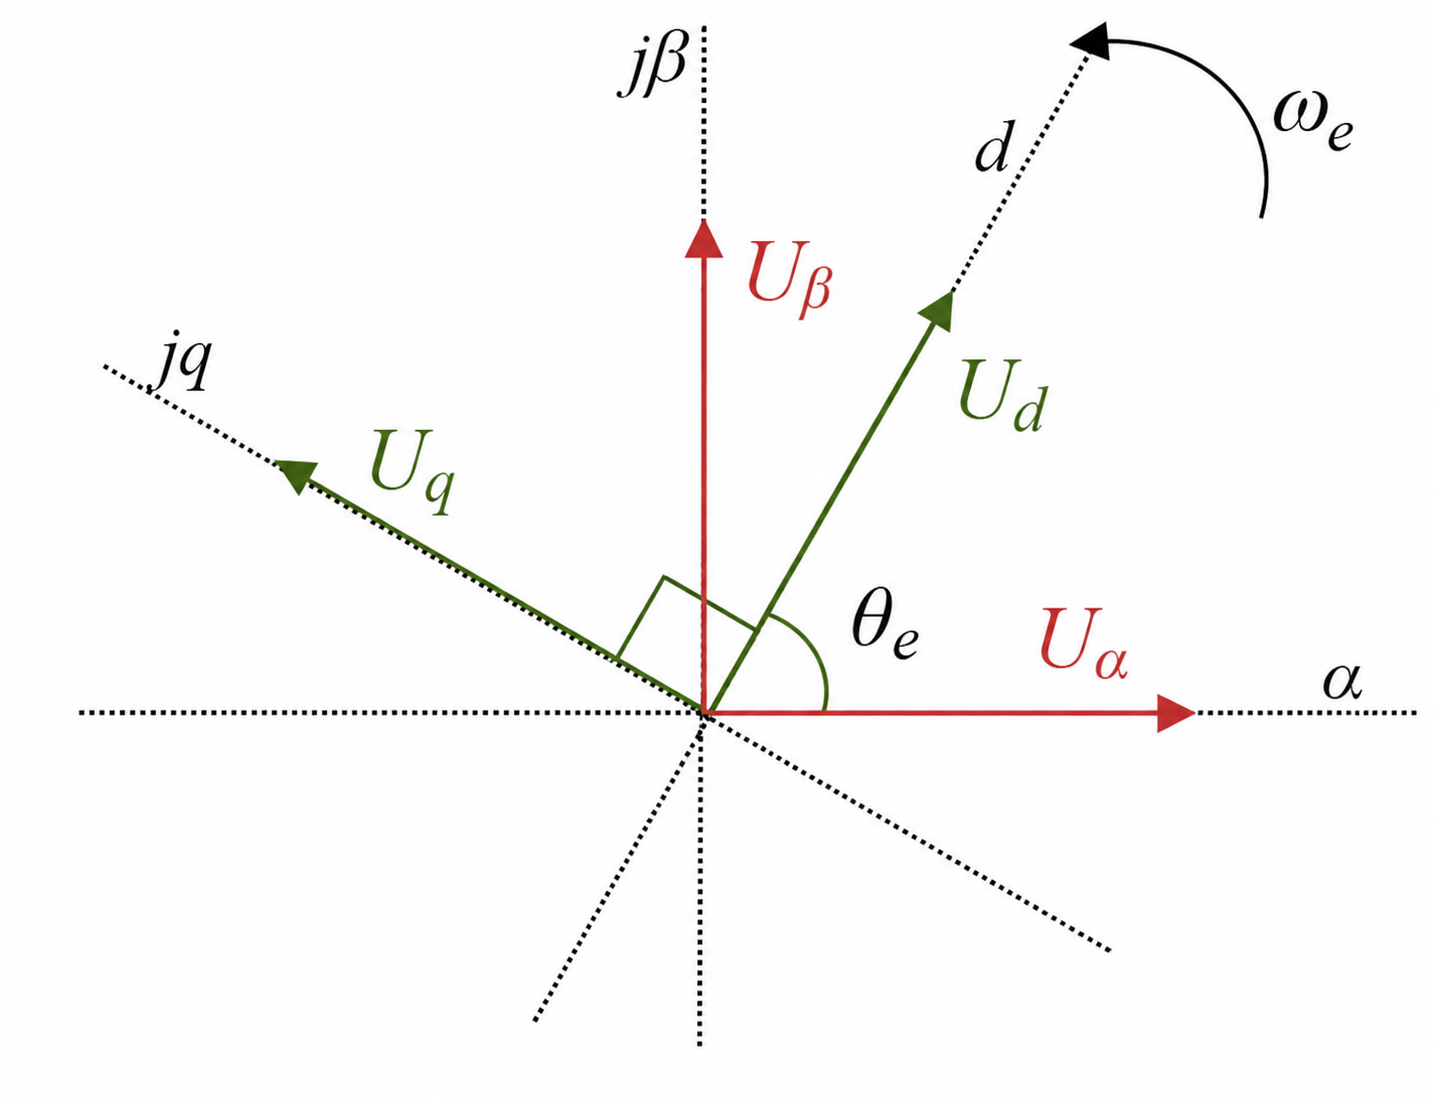
\includegraphics[width=0.5\linewidth]{dq-image.png}
    \caption{$dq$ and $\alpha\beta$ Frames}
    \label{fig:dq-alpha-beta}
\end{figure}


%=========================================================================%
\subsubsection{Park Transformation}
\label{sec-park-transformation}

The Park transformation can be understood geometrically as a rotation of the stationary $\alpha\beta0$ coordinate system about the zero-sequence axis. The $dq$ coordinate system rotates through the rotor electrical angle $\theta_{e}$, while the zero-sequence axis remains unchanged.

We begin with the stationary $\alpha\beta0$ basis vectors:

\begin{equation}
    \hat{\boldsymbol{\alpha}}
    =
    \begin{bmatrix}
        1 \\
        0 \\
        0
    \end{bmatrix},
    \qquad
    \hat{\boldsymbol{\beta}}
    =
    \begin{bmatrix}
        0 \\
        1 \\
        0
    \end{bmatrix},
    \qquad
    \hat{\mathbf{0}}
    =
    \begin{bmatrix}
        0 \\
        0 \\
        1
    \end{bmatrix}
\end{equation}

For rotor-oriented control, the $d$-axis is defined to be aligned with the :permanent-magnet flux-linkage vector. Recall that in the stationary $\alpha\beta$ frame:

\begin{equation}
    \boldsymbol{\lambda}_{m,\alpha\beta}
    =
    \lambda_m
    \begin{bmatrix}
        \cos(\theta_e) \\
        \sin(\theta_e)
    \end{bmatrix}
\end{equation}

The direction of the $d$-axis in the $\alpha\beta0$ coordinate system is therefore:

\begin{equation}
    \hat{\mathbf{d}}
    =
    \begin{bmatrix}
        \cos(\theta_{e}) \\
        \sin(\theta_{e}) \\
        0
    \end{bmatrix}
\end{equation}

The $q$-axis is defined to be perpendicular to the $d$-axis and displaced by $+90^\circ$ electrical in the direction of rotation. Its direction is therefore:

\begin{equation}
    \hat{\mathbf{q}}
    =
    \begin{bmatrix}
        \cos\left(\theta_{e}+\frac{\pi}{2}\right) \\
        \sin\left(\theta_{e}+\frac{\pi}{2}\right) \\
        0
    \end{bmatrix}
\end{equation}

Using:

\begin{align}
    \cos\left(\theta+\frac{\pi}{2}\right) &= -\sin(\theta), \\
    \sin\left(\theta+\frac{\pi}{2}\right) &= \cos(\theta),
\end{align}

the $q$-axis becomes:

\begin{equation}
    \hat{\mathbf{q}}
    =
    \begin{bmatrix}
        -\sin(\theta_{e}) \\
        \cos(\theta_{e}) \\
        0
    \end{bmatrix}
\end{equation}

Because the $dq$ coordinate system is obtained by rotating about the zero-sequence axis, the zero-sequence basis vector itself is unchanged:

\begin{equation}
    \hat{\mathbf{0}}_{dq}
    =
    \begin{bmatrix}
        0 \\
        0 \\
        1
    \end{bmatrix}
\end{equation}

These vectors, $\mathbf{\hat{d}}$, $\mathbf{\hat{q}}$, $\mathbf{\hat{0}}_{dq}$, represent the new basis vectors as expressed in the $\alpha\beta$ frame, similar to Section \ref{geometric-interpretation} in the Clarke transformation derivation. We can see from Figure \ref{fig:dq-alpha-beta} using trigonometry that, with respect to the $\alpha\beta$ frame, the coordinates of the $\mathbf{\hat{d}}$-axis have components on the $\alpha$ and $\beta$ axis of $\cos(\theta_e)$ and $\sin(\theta_e)$, respectively.

Similarly, the components of the $\mathbf{\hat{q}}$-axis has components of:

\begin{equation}
    q_\alpha = -\cos(\pi - \frac{\pi}{2} - \theta_e) = -\cos(\frac{\pi}{2} - \theta_e) = -\sin(\theta_e)
\end{equation}

\begin{equation}
    q_\beta = \sin(\pi - \frac{\pi}{2} - \theta_e) = \sin(\frac{\pi}{2} - \theta_e) = \cos(\theta_e)
\end{equation}

However, since we have found the $dq$ vectors as seen in the $\alpha\beta$ frame, this yields the transformation matrix that converts vectors in $dq$ frame to $\alpha\beta$ frame. In other words, the inverse Park transform, using a general angle, $\theta$:

\begin{equation}
    \hat{\mathbf{d}}
    =
    \begin{bmatrix}
        \cos(\theta) \\
        \sin(\theta) \\
        0
    \end{bmatrix},
    \qquad
    \hat{\mathbf{q}}
    =
    \begin{bmatrix}
        -\sin(\theta) \\
        \cos(\theta) \\
        0
    \end{bmatrix},
    \qquad
    \hat{\mathbf{0}}_{dq}
    =
    \begin{bmatrix}
        0 \\
        0 \\
        1
    \end{bmatrix}.
\end{equation}

\begin{equation}
    \mathbf{T}_p^{-1}
    =
    \begin{bmatrix}
        \cos(\theta) & -\sin(\theta) & 0 \\
        \sin(\theta) & \cos(\theta) & 0 \\
        0 & 0 & 1
    \end{bmatrix}
\end{equation}

Thus:

\begin{equation}
    \mathbf{f}_{\alpha\beta0}
    =
    \mathbf{T}_p^{-1}\mathbf{f}_{dq0}.
\end{equation}

The $dq0$ basis vectors are mutually perpendicular and each have unit magnitude. The transformation matrix is therefore orthogonal, meaning that its inverse is equal to its transpose:

\begin{equation}
    \mathbf{T}_p^{-1}
    =
    \mathbf{T}_p^T.
\end{equation}

Taking the transpose therefore gives the forward Park transformation:

\begin{equation}
    \mathbf{T}_p
    =
    \begin{bmatrix}
        \cos(\theta) & \sin(\theta) & 0 \\
        -\sin(\theta) & \cos(\theta) & 0 \\
        0 & 0 & 1
    \end{bmatrix}
\end{equation}

Therefore:

\begin{equation}
    \mathbf{f}_{dq0}
    =
    \mathbf{T}_p\mathbf{f}_{\alpha\beta0}
\end{equation}

In matrix form:

\begin{equation}
    \begin{bmatrix}
        f_d \\
        f_q \\
        f_0
    \end{bmatrix}
    =
    \begin{bmatrix}
        \cos(\theta) & \sin(\theta) & 0 \\
        -\sin(\theta) & \cos(\theta) & 0 \\
        0 & 0 & 1
    \end{bmatrix}
    \begin{bmatrix}
        f_\alpha \\
        f_\beta \\
        f_0
    \end{bmatrix}
\end{equation}

Substituting the results from Section \ref{sec-amp-invar-clarke}, where for a balanced three phase quantity in $abc$ frame, $\mathbf{f}_{\alpha\beta0}$ is:

\begin{equation}
    \begin{bmatrix}
        f_\alpha \\
        f_\beta \\
        f_0
    \end{bmatrix}
    =
    \begin{bmatrix}
        F\cos(\theta) \\
        F\sin(\theta) \\
        0
    \end{bmatrix}
\end{equation}

\begin{align}
    \begin{bmatrix}
        f_d \\
        f_q \\
        f_0
    \end{bmatrix}
    &=
    \begin{bmatrix}
        \cos(\theta) & \sin(\theta) & 0 \\
        -\sin(\theta) & \cos(\theta) & 0 \\
        0 & 0 & 1
    \end{bmatrix}
    \begin{bmatrix}
        F\cos(\theta) \\
        F\sin(\theta) \\
        0
    \end{bmatrix} \\[8pt]
    &=
    \begin{bmatrix}
        F(\cos^2(\theta) + \sin^2(\theta)) \\
        F(-\cos(\theta)\sin(\theta) + \sin(\theta)\cos(\theta)) \\
        0
    \end{bmatrix} \\[8pt]
    &=
    \begin{bmatrix}
        F \\
        0 \\
        0
    \end{bmatrix}
\end{align}

Now we can see that for balanced, three phase currents in $abc$ frame, performing an amplitude invariant Clarke transform, then a Park transform, simplifies the three dimensional sinusoidal currents to a single DC value.

The Park transformation was derived above using the complete $\alpha\beta0$ and $dq0$ coordinate systems in order to clearly show its geometric formulation. In particular, the transformation represents a rotation about the zero-sequence axis, leaving the zero-sequence component unchanged:

\begin{equation}
    f_{0,dq} = f_{0,\alpha\beta}
\end{equation}

However, as established during the derivation of the Clarke transformation and prior, the balanced PMSM considered here has no zero-sequence component. Therefore:

\begin{equation}
    f_0 = 0
\end{equation}

Since the Park transformation neither creates nor modifies a zero-sequence component, the zero-sequence axis can once again be disregarded. The transformation can therefore be reduced from the three-dimensional $dq0$ form to the two-dimensional $dq$ form, preserving this benefit from the Clarke transformation:

\begin{equation}
    \begin{bmatrix}
        f_d \\
        f_q
    \end{bmatrix}
    =
    \begin{bmatrix}
        \cos(\theta) & \sin(\theta) \\
        -\sin(\theta) & \cos(\theta)
    \end{bmatrix}
    \begin{bmatrix}
        f_\alpha \\
        f_\beta
    \end{bmatrix}
\end{equation}

The reduced Park transformation matrix is therefore:

\begin{equation}
    \mathbf{T}_p
    =
    \begin{bmatrix}
        \cos(\theta) & \sin(\theta) \\
        -\sin(\theta) & \cos(\theta)
    \end{bmatrix}
\end{equation}

Unlike the reduced Clarke transformation, the reduced Park transformation remains square and orthogonal. Its inverse is therefore simply its transpose:

\begin{equation}
\label{eqn-inv-park}
    \mathbf{T}_p^{-1}
    =
    \mathbf{T}_p^T
    =
    \begin{bmatrix}
        \cos(\theta) & -\sin(\theta) \\
        \sin(\theta) & \cos(\theta)
    \end{bmatrix}
\end{equation}


%=========================================================================%
\subsubsection{Transformation of the PMSM Model}
%=========================================================================%

%=========================================================================%
\paragraph{Voltage Equations in \texorpdfstring{$dq$}{dq} Frame}
%=========================================================================%


Recall the equations for a PMSM in $\alpha\beta$ frame:

\begin{equation}
    \mathbf{v}_{\alpha\beta}
    =
    R_s\mathbf{i}_{\alpha\beta}
    +
    \mathbf{L}_{\alpha\beta}
    \frac{d\mathbf{i}_{\alpha\beta}}{dt}
    +
    \mathbf{e}_{\alpha\beta}
\end{equation}

If we instead write this in terms of flux linkage:

\begin{equation}
    \mathbf{v}_{\alpha\beta}
    =
    R_s\mathbf{i}_{\alpha\beta}
    +
    \frac{d\boldsymbol{\lambda}_{\alpha\beta}}{dt}
\end{equation}

Where:

\begin{equation}
\label{eqn-alpha-beta-total-flux}
    \boldsymbol{\lambda}_{\alpha\beta} = \mathbf{L}_{\alpha\beta}\mathbf{i}_{\alpha\beta} + \boldsymbol{\lambda}_{m,\alpha\beta}
\end{equation}

We will return to the $\alpha\beta$ flux linkage transformation later. Multiplying each side by the Park transformation matrix:

\begin{equation}
    \mathbf{T}_p\mathbf{v}_{\alpha\beta}
    =
    \mathbf{T}_pR_s\mathbf{i}_{\alpha\beta}
    +
    \mathbf{T}_p\frac{d\boldsymbol{\lambda}_{\alpha\beta}}{dt}
\end{equation}

Using the Park transformation:

\begin{equation}
    \mathbf{v}_{dq} = \mathbf{T}_p\mathbf{v}_{\alpha\beta}, \qquad
    \mathbf{i}_{dq} = \mathbf{T}_p\mathbf{i}_{\alpha\beta}
\end{equation}

\begin{equation}
\label{eqn-dq-intermediate1}
    \mathbf{v}_{dq}
    =
    R_s\mathbf{i}_{dq}
    +
    \mathbf{T}_p\frac{d\boldsymbol{\lambda}_{\alpha\beta}}{dt}
\end{equation}

If we define:

\begin{equation}
\label{eqn-dq-ab-flux-park}
    \boldsymbol{\lambda}_{dq} = \mathbf{T}_p\boldsymbol{\lambda}_{\alpha\beta}
\end{equation}

Since we are using electrical quantities, the Park transform is therefore dependent on electrical angle, $\theta = \theta_e(t)$, which varies with time. We must take this into account in the derivative:

\begin{align}
    \frac{d\boldsymbol{\lambda}_{dq}}{dt} 
    &= \frac{d}{dt}(\mathbf{T}_p\boldsymbol{\lambda}_{\alpha\beta}) \\[6pt]
    &= \frac{d\mathbf{T}_p}{dt}\boldsymbol{\lambda}_{\alpha\beta} + \mathbf{T}_p\frac{d\boldsymbol{\lambda}_{\alpha\beta}}{dt}
\end{align}

Rearranging we get:

\begin{equation}
    \mathbf{T}_p\frac{d\boldsymbol{\lambda}_{\alpha\beta}}{dt} = \frac{d\boldsymbol{\lambda}_{dq}}{dt} - \frac{d\mathbf{T}_p}{dt}\boldsymbol{\lambda}_{\alpha\beta}
\end{equation}

Then substituting:

\begin{equation}
    \boldsymbol{\lambda}_{\alpha\beta} = \mathbf{T}_p^{-1}\boldsymbol{\lambda}_{dq}
\end{equation}

\begin{equation}
    \mathbf{T}_p\frac{d\boldsymbol{\lambda}_{\alpha\beta}}{dt} = \frac{d\boldsymbol{\lambda}_{dq}}{dt} - \frac{d\mathbf{T}_p}{dt}\mathbf{T}_p^{-1}\boldsymbol{\lambda}_{dq}
\end{equation}

Recall that:

\begin{equation}
    \frac{d\theta_e}{dt} = \omega_e
\end{equation}

If we evaluate the second term on the right hand side, beginning with the derivative of the Park transform:

\begin{align}
    \frac{d\mathbf{T}_p}{dt} &= \frac{d}{dt} \left(
    \begin{bmatrix}
        \cos(\theta_e) & \sin(\theta_e) \\
        -\sin(\theta_e) & \cos(\theta_e)
    \end{bmatrix}
    \right) \\[6pt]
    &= \omega_e
    \begin{bmatrix}
        -\sin(\theta_e) & \cos(\theta_e) \\
        -\cos(\theta_e) & -\sin(\theta_e)
    \end{bmatrix}
\end{align}

From Equation \ref{eqn-inv-park}:

\begin{equation}
    \mathbf{T}_p^{-1}
    =
    \begin{bmatrix}
        \cos(\theta) & -\sin(\theta) \\
        \sin(\theta) & \cos(\theta)
    \end{bmatrix}
\end{equation}

Then:

\begin{align}
    \frac{d\mathbf{T}_p}{dt}\mathbf{T}_p^{{-1}} &=
    \omega_e
    \begin{bmatrix}
        -\sin(\theta_e) & \cos(\theta_e) \\
        -\cos(\theta_e) & -\sin(\theta_e)
    \end{bmatrix}
        \begin{bmatrix}
        \cos(\theta) & -\sin(\theta) \\
        \sin(\theta) & \cos(\theta)
    \end{bmatrix} \\[6pt]
    &= \omega_e
    \begin{bmatrix}
        0 & 1 \\
        -1 & 0
    \end{bmatrix}
\end{align}

Define the $90^\circ$ rotation matrix, $\mathbf{J}$:

\begin{equation}
    \mathbf{J} =
    \begin{bmatrix}
        0 & -1 \\
        1 & 0
    \end{bmatrix}
\end{equation}

Then:

\begin{equation}
    -\frac{d\mathbf{T}_p}{dt}\mathbf{T}_p^{{-1}} = \omega_e\mathbf{J}
\end{equation}

Finally, we have that:

\begin{equation}
    \mathbf{T}_p\frac{d\boldsymbol{\lambda}_{\alpha\beta}}{dt} = \frac{d\boldsymbol{\lambda}_{dq}}{dt} + \omega_e\mathbf{J}\boldsymbol{\lambda}_{dq}
\end{equation}

Putting it all together using Equation \ref{eqn-dq-intermediate1}:

\begin{equation}
    \mathbf{v}_{dq}
    =
    R_s\mathbf{i}_{dq}
    +
    \frac{d\boldsymbol{\lambda}_{dq}}{dt} + \omega_eJ\boldsymbol{\lambda}_{dq}
\end{equation}

Or explicitly, in matrix form:

\begin{equation}
\label{eqn-dq-equations-flux-matrix-form}
    \begin{bmatrix}
        v_d \\
        vq
    \end{bmatrix}
    = R_s
    \begin{bmatrix}
        i_d \\
        i_q
    \end{bmatrix}
    +
    \frac{d}{dt}
    \begin{bmatrix}
        \lambda_d \\
        \lambda_q
    \end{bmatrix}
    + \omega_e
    \begin{bmatrix}
        0 & -1 \\
        1 & 0
    \end{bmatrix}
    \begin{bmatrix}
        \lambda_d \\
        \lambda_q
    \end{bmatrix}
\end{equation}

Multiplying out:

\begin{equation}
\label{eqn-vd-in-terms-of-flux}
    v_d = R_si_d + \frac{d\lambda_d}{dt} - \omega_e\lambda_q
\end{equation}

\begin{equation}
\label{eqn-vq-in-terms-of-flux}
    v_q = R_si_q + \frac{d\lambda_q}{dt} + \omega_e\lambda_d
\end{equation}


%=========================================================================%
\paragraph{Flux Linkages in the \texorpdfstring{$dq$}{dq} Frame}
%=========================================================================%

Equations \ref{eqn-vd-in-terms-of-flux} and \ref{eqn-vq-in-terms-of-flux} express the stator voltage equations in the rotating $dq$ reference frame in terms of the $d$ and $q$-axis flux linkages. To obtain the equations explicitly in terms of the stator currents and permanent-magnet flux, the flux-linkage vector must now be expressed in the \(dq\) frame.

Recall from Equation \ref{eqn-alpha-beta-total-flux} that:

\begin{equation}
    \boldsymbol{\lambda}_{\alpha\beta} = \mathbf{L}_{\alpha\beta}\mathbf{i}_{\alpha\beta} + \boldsymbol{\lambda}_{m,\alpha\beta}
\end{equation}

And from Equation \ref{eqn-dq-ab-flux-park} that:

\begin{equation}
    \boldsymbol{\lambda}_{dq} = \mathbf{T}_p\boldsymbol{\lambda}_{\alpha\beta}
\end{equation}

Substituting the expression for total flux linkage:

\begin{align}
    \boldsymbol{\lambda}_{dq} 
    &= 
    \mathbf{T}_p(\mathbf{L}_{\alpha\beta}\mathbf{i}_{\alpha\beta} + \boldsymbol{\lambda}_{m,\alpha\beta}) \\[4pt]
    &=
    \mathbf{T}_p\mathbf{L}_{\alpha\beta}\mathbf{i}_{\alpha\beta} + \mathbf{T}_p\boldsymbol{\lambda}_{m,\alpha\beta}
\end{align}

From the inverse Park transform:

\begin{equation}
    \mathbf{i}_{\alpha\beta} = \mathbf{T}_p^{-1}\mathbf{i}_{dq}
\end{equation}

Therefore:

\begin{equation}
    \boldsymbol{\lambda}_{dq} 
    =
    \mathbf{T}_p\mathbf{L}_{\alpha\beta}\mathbf{T}_p^{-1}\mathbf{i}_{dq} + \mathbf{T}_p\boldsymbol{\lambda}_{m,\alpha\beta}
\end{equation}

Now, we define the Park transformed inductance matrix:

\begin{equation}
    \mathbf{L}_{dq} = \mathbf{T}_p\mathbf{L}_{\alpha\beta}\mathbf{T}_p^{-1}
\end{equation}

Recall from Equation \ref{eqn-alpha-beta-inductance-matrix} the inductance matrix in $\alpha\beta$ frame:

\begin{equation}
    \mathbf{L}_{\alpha\beta} =
    \begin{bmatrix}
        L_\alpha & 0 \\
        0 & L_\beta
    \end{bmatrix}
\end{equation}

Where, from Equation \ref{eqn-Lalpha-Lbeta}, for a non salient PMSM:

\begin{equation}
    L_\alpha = L_\beta = \frac{3}{2}L_s
\end{equation}

Substituting the Park transformation, the $\alpha\beta$ inductance matrix,
and the inverse Park transformation:

\begin{align}
    \mathbf{L}_{dq}
    &=
    \begin{bmatrix}
        \cos(\theta_e) & \sin(\theta_e) \\
        -\sin(\theta_e) & \cos(\theta_e)
    \end{bmatrix}
    \begin{bmatrix}
        L_\alpha & 0 \\
        0 & L_\beta
    \end{bmatrix}
    \begin{bmatrix}
        \cos(\theta_e) & -\sin(\theta_e) \\
        \sin(\theta_e) & \cos(\theta_e)
    \end{bmatrix}
\end{align}

Evaluating the first matrix multiplication:

\begin{align}
    \mathbf{L}_{dq}
    &=
    \begin{bmatrix}
        L_\alpha \cos(\theta_e) & L_\beta \sin(\theta_e) \\
        -L_\alpha \sin(\theta_e) & L_\beta \cos(\theta_e)
    \end{bmatrix}
    \begin{bmatrix}
        \cos(\theta_e) & -\sin(\theta_e) \\
        \sin(\theta_e) & \cos(\theta_e)
    \end{bmatrix}
\end{align}

Multiplying the remaining matrices:

\begin{align}
    \mathbf{L}_{dq}
    =
    \begin{bmatrix}
        L_\alpha \cos^2(\theta_e)
        + L_\beta \sin^2(\theta_e)
        &
        (L_\beta-L_\alpha)
        \sin(\theta_e)\cos(\theta_e)
        \\[6pt]
        (L_\beta-L_\alpha)
        \sin(\theta_e)\cos(\theta_e)
        &
        L_\alpha \sin^2(\theta_e)
        + L_\beta \cos^2(\theta_e)
    \end{bmatrix}
\end{align}

Since for the non-salient PMSM considered here:

\begin{align}
    L_\alpha = L_\beta
\end{align}

the off-diagonal terms become:

\begin{align}
    (L_\beta-L_\alpha)
    \sin(\theta_e)\cos(\theta_e)
    = 0
\end{align}

The diagonal terms simplify using:

\begin{align}
    \cos^2(\theta_e)+\sin^2(\theta_e)=1
\end{align}

such that:

\begin{align}
    L_\alpha\cos^2(\theta_e)
    +L_\beta\sin^2(\theta_e)
    &=
    L_\alpha
    \left(
        \cos^2(\theta_e)+\sin^2(\theta_e)
    \right)
    \\
    &=L_\alpha
\end{align}

and similarly:

\begin{align}
    L_\alpha\sin^2(\theta_e)
    +L_\beta\cos^2(\theta_e)
    &=
    L_\beta
    \left(
        \sin^2(\theta_e)+\cos^2(\theta_e)
    \right)
    \\
    &=L_\beta
\end{align}

For the sake of consistency, we denote:

\begin{equation}
    L_d = L_\alpha
\end{equation}

And:

\begin{equation}
    L_q = L_\beta
\end{equation}

Therefor:

\begin{equation}
    L_d = L_q
\end{equation}

For a non-salient PMSM. The inductance matrix in the $dq$ frame is then:

\begin{align}
    \mathbf{L}_{dq}
    =
    \begin{bmatrix}
        L_d & 0 \\
        0 & L_q
    \end{bmatrix}
\end{align}

From Equation \ref{eqn-alpha-beta-pm-flux}, we know the permanent magnet flux linkages in $\alpha\beta$ frame is:

\begin{equation}
    \boldsymbol{\lambda}_{m,\alpha\beta}
    =
    \lambda_m
    \begin{bmatrix}
        \cos(\theta_e) \\
        \sin(\theta_e)
    \end{bmatrix}
\end{equation}

Then, using the general Park transform solution for this type of vector derived in Section \ref{sec-park-transformation}:

\begin{equation}
    \boldsymbol{\lambda}_{dq} = \mathbf{T}_p\boldsymbol{\lambda}_{\alpha\beta}
\end{equation}

\begin{equation}
    \begin{bmatrix}
        \lambda_{m,d} \\
        \lambda_{m,q}
    \end{bmatrix}
    =
    \begin{bmatrix}
        \lambda_m \\
        0
    \end{bmatrix}
\end{equation}

Note that like we have defined, the permanent magnet flux linkage lies entirely along the direct axis. The total flux linkage is then:

\begin{equation}
    \boldsymbol{\lambda}_{dq} = \mathbf{L}_{dq}\mathbf{i}_{dq} + \boldsymbol{\lambda}_{m,dq}
\end{equation}

In matrix form:

\begin{equation}
\label{eqn-dq-flux-matrix-form}
    \begin{bmatrix}
        \lambda_d \\
        \lambda_q
    \end{bmatrix}
    =
    \begin{bmatrix}
        L_d & 0 \\
        0 & L_q
    \end{bmatrix}
    \begin{bmatrix}
        i_d \\
        i_q
    \end{bmatrix}
    +
    \begin{bmatrix}
        \lambda_m \\
        0
    \end{bmatrix}
\end{equation}

%=========================================================================%
\subsubsection{PMSM Equations in \texorpdfstring{$dq$}{dq} Frame}
%=========================================================================%


From Equations \ref{eqn-vd-in-terms-of-flux} and \ref{eqn-vq-in-terms-of-flux}:

\begin{equation}
    v_d = R_si_d + \frac{d\lambda_d}{dt} - \omega_e\lambda_q
\end{equation}

\begin{equation}
    v_q = R_si_q + \frac{d\lambda_q}{dt} + \omega_e\lambda_d
\end{equation}

From Equation \ref{eqn-dq-flux-matrix-form} and expanding:

\begin{equation}
    \lambda_d = L_d i_d + \lambda_m
\end{equation}

\begin{equation}
    \lambda_q = L_q i_q
\end{equation}

Evaluating the derivative yields:

\begin{equation}
    \frac{d\lambda_d}{dt} = L_d\frac{di_d}{dt}
\end{equation}

\begin{equation}
    \frac{d\lambda_q}{dt} = L_q\frac{di_q}{dt}
\end{equation}

Substituting this for the derivative terms and multiplying out the cross coupling terms:

\begin{equation}
    v_d = R_si_d + L_d\frac{di_d}{dt} - \omega_eL_qi_q
\end{equation}

\begin{equation}
    v_q = R_si_q + Lq\frac{di_q}{dt} + \omega_eL_di_d + \omega_e\lambda_m
\end{equation}

Observe the different components of these equations: There is a resistive component associated with the losses from the stator resistance, the inductive voltage terms representing the voltage required to change the stator currents, the cross coupling terms and the back-EMF term only associated with the $q$-axis.

The cross coupling terms are of particular note since this means our equations are not independent. Thus $d$- and $q$-axis voltages can not be individually controlled; A commanded current on one axis will affect the other, while the strength of this effect is proportional to the electrical speed.

The back-EMF term appears only along the $q$-axis since we have defined the direct axis to be in the direction of the rotor flux. Because back-EMF is proportional to the derivative of the rotor flux, the back-EMF leads the $d$-axis by $90^\circ$.



%=========================================================================%
\paragraph{Summary}
%=========================================================================%
For the balanced PMSM considered here, the Park transformation rotates quantities from the stationary $\alpha\beta$ reference frame into the synchronous $dq$ reference frame. For rotor oriented control, the transformation angle is chosen as the rotor electrical angle, $\theta = \theta_e$, such that the $d$-axis remains aligned with the permanent magnet flux linkage vector.

The forward Park transformation is:

\begin{equation}
    \mathbf{f}_{dq}
    =
    \mathbf{T}_p\mathbf{f}_{\alpha\beta}
\end{equation}

In matrix form:

\begin{equation}
    \begin{bmatrix}
        f_d \\
        f_q
    \end{bmatrix}
    =
    \begin{bmatrix}
        \cos(\theta) & \sin(\theta) \\
        -\sin(\theta) & \cos(\theta)
    \end{bmatrix}
    \begin{bmatrix}
        f_\alpha \\
        f_\beta
    \end{bmatrix}
\end{equation}

Where:

\begin{equation}
    \mathbf{T}_p
    =
    \begin{bmatrix}
        \cos(\theta) & \sin(\theta) \\
        -\sin(\theta) & \cos(\theta)
    \end{bmatrix}
\end{equation}

The inverse Park transformation is:

\begin{equation}
    \mathbf{f}_{\alpha\beta}
    =
    \mathbf{T}_p^{-1}\mathbf{f}_{dq}
\end{equation}

In matrix form:

\begin{equation}
    \begin{bmatrix}
        f_\alpha \\
        f_\beta
    \end{bmatrix}
    =
    \begin{bmatrix}
        \cos(\theta) & -\sin(\theta) \\
        \sin(\theta) & \cos(\theta)
    \end{bmatrix}
    \begin{bmatrix}
        f_d \\
        f_q
    \end{bmatrix}
\end{equation}

where:

\begin{equation}
    \mathbf{T}_p^{-1}
    =
    \mathbf{T}_p^T
\end{equation}

The general stator voltage equation in the rotating $dq$ frame is:

\begin{equation}
    \mathbf{v}_{dq} = R_s\mathbf{i}_{dq} + \frac{d\boldsymbol{\lambda}_{dq}}{dt} + \omega_e\mathbf{J}\boldsymbol{\lambda}_{dq}
\end{equation}

The total stator flux linkage in $dq$ frame is:

\begin{equation}
    \boldsymbol{\lambda}_{dq} = \mathbf{L}_{dq}\mathbf{i}_{dq} + \boldsymbol{\lambda}_{m,dq}
\end{equation}

Where:

\begin{equation}
    \mathbf{L}_{dq} =
    \begin{bmatrix}
        L_d & 0 \\
        0 & L_q 
    \end{bmatrix},
    \qquad
    \boldsymbol{\lambda}_{m,dq} = 
    \begin{bmatrix}
        \lambda_{m} \\
        0
    \end{bmatrix}
\end{equation}

Giving:

\begin{equation}
    \lambda_d = L_di_d + \lambda_m
\end{equation}

\begin{equation}
    \lambda_q = L_qi_q
\end{equation}

For the non-salient machine considered here:

\begin{equation}
    L_d = L_q = L_\alpha = L_\beta = \frac{3}{2}L_s
\end{equation}

And the $90^\circ$ rotation matrix, $\mathbf{J}$, is:

\begin{equation}
    \mathbf{J} =
    \begin{bmatrix}
        0 & -1 \\
        1 & 0
    \end{bmatrix}
\end{equation}

Substituting the above leads to the final PMSM voltage equations:

\begin{equation}
\label{eqn-vd}
    v_d = R_si_d + L_d\frac{di_d}{dt} - \omega_eL_qi_q
\end{equation}

\begin{equation}
\label{eqn-vq}
    v_q = R_si_q + L_q\frac{di_q}{dt} + \omega_eL_di_d + \omega_e\lambda_m
\end{equation}

%=========================================================================%
\subsection{Electromechanical Model}
\label{sec:electromechanical-model}

\subsubsection{Electromechanical Power}
\label{sec:electromechanical-power}
%=========================================================================%

In a three phase system, the input electrical power is:

\begin{equation}
\label{eqn-abc-power}
    P_{abc} = v_ai_a + v_bi_b + v_ci_c
\end{equation}

Or:

\begin{equation}
\label{eqn-abc-power-dot-product}
    P_{abc} = \mathbf{v}_{abc}^T\mathbf{i}_{abc}
\end{equation}

Using the amplitude invariant Clarke transform from Section \ref{sec-amp-invar-clarke}, recall that:

\begin{equation}
\label{eqn-inverse-clarke-transpose}
    \mathbf{T}_c^{-1} = \frac{3}{2}\mathbf{T}_c^T
\end{equation}

And:

\begin{equation}
    \mathbf{v}_{abc} = \mathbf{T}_c^{-1}\mathbf{v}_{\alpha\beta}, \qquad
    \mathbf{i}_{abc} = \mathbf{T}_c^{-1}\mathbf{i}_{\alpha\beta}
\end{equation}

Given that:

\begin{equation}
    (\mathbf{AB})^T = \mathbf{B}^T\mathbf{A}^T
\end{equation}

Therefore:

\begin{align}
    P_{abc} 
    &= (\mathbf{T}_c^{-1}\mathbf{v}_{\alpha\beta})^T (\mathbf{T}_c^{-1}\mathbf{i}_{\alpha\beta}) \\[6pt]
    &= \mathbf{v}_{\alpha\beta}^T(\mathbf{T}_c^{-1})^T\mathbf{T}_c^{-1}\mathbf{i}_{\alpha\beta}
\end{align}

Evaluating $(\mathbf{T}_c^{-1})^T\mathbf{T}_c^{-1}$, using the relationship in Equation \ref{eqn-inverse-clarke-transpose}:

\begin{equation}
    (\mathbf{T}_c^{-1})^T\mathbf{T}_c^{-1} = (\frac{3}{2}\mathbf{T}_c^T)^T\mathbf{T}_c^{-1} = \frac{3}{2}\mathbf{T}_c\mathbf{T}_c^{-1} = \frac{3}{2}\mathbf{I}
\end{equation}

Where $\mathbf{I}$ is the identity matrix. Then:

\begin{equation}
    P_{abc} = \mathbf{v}_{\alpha\beta}^T(\frac{3}{2}\mathbf{I})\mathbf{i}_{\alpha\beta}
\end{equation}

Therefore:

\begin{equation}
    P_{abc} = \frac{3}{2}\mathbf{v}_{\alpha\beta}^T\mathbf{i}_{\alpha\beta}
\end{equation}

Note that the $3/2$ term appears as a result of our choice to use the amplitude invariant Clarke transform. Should we have used the power invariant Clarke transform, which preserves the dot product, this factor would not appear. Next, converting to $dq$ frame, recall that:

\begin{equation}
    \mathbf{v}_{\alpha\beta} = \mathbf{T}_p^{-1}\mathbf{v}_{dq}, \qquad
    \mathbf{i}_{\alpha\beta} = \mathbf{T}_p^{-1}\mathbf{i}_{dq}
\end{equation}

And:

\begin{equation}
    \mathbf{T}_p^{-1} = \mathbf{T}_p^T
\end{equation}

Therefore:

\begin{align}
    P_{abc} 
    &= \frac{3}{2}(\mathbf{T}_p^{-1}\mathbf{v}_{dq})^T(\mathbf{T}_p^{-1}\mathbf{i}_{dq}) \\[4pt]
    &= \frac{3}{2}\mathbf{v}_{dq}^T(\mathbf{T}_p^{-1})^T\mathbf{T}_p^{-1}\mathbf{i}_{dq} \\[4pt]
    &= \frac{3}{2}\mathbf{v}_{dq}^T\mathbf{T}_p\mathbf{T}_p^{-1}\mathbf{i}_{dq} \\[4pt]
    &= \frac{3}{2}\mathbf{v}_{dq}^T\mathbf{I}\mathbf{i}_{dq} \\[4pt]
    &= \frac{3}{2}\mathbf{v}_{dq}^T\mathbf{i}_{dq}
\end{align}

Finally:

\begin{equation}
    P_{abc} = \frac{3}{2}(v_di_d + v_qi_q)
\end{equation}

Recall from Equations \ref{eqn-vd} and \ref{eqn-vq}:

\begin{equation}
    v_d = R_si_d + L_d\frac{di_d}{dt} - \omega_eL_qi_q
\end{equation}

\begin{equation}
    v_q = R_si_q + L_q\frac{di_q}{dt} + \omega_eL_di_d + \omega_e\lambda_m
\end{equation}

Substituting the $dq$ voltage equations into the power equation:

\begin{align}
P_{abc}
&=
\frac{3}{2}
\left[
\left(
R_s i_d
+
L_d\frac{di_d}{dt}
-
\omega_e L_q i_q
\right)i_d
+
\left(
R_s i_q
+
L_q\frac{di_q}{dt}
+
\omega_e L_d i_d
+
\omega_e\lambda_m
\right)i_q
\right]
\\[6pt]
&=
\frac{3}{2}
\left[
R_s i_d^2
+
L_d i_d\frac{di_d}{dt}
-
\omega_e L_q i_d i_q
+
R_s i_q^2
+
L_q i_q\frac{di_q}{dt}
+
\omega_e L_d i_d i_q
+
\omega_e\lambda_m i_q
\right]
\\[6pt]
&=
\frac{3}{2}
\left[
R_s(i_d^2+i_q^2)
+
L_d i_d\frac{di_d}{dt}
+
L_q i_q\frac{di_q}{dt}
+
\omega_e(L_d-L_q)i_d i_q
+
\omega_e\lambda_m i_q
\right]
\\[6pt]
&=
\frac{3}{2}R_s(i_d^2+i_q^2)
+
\frac{3}{2}
\left(
L_d i_d\frac{di_d}{dt}
+
L_q i_q\frac{di_q}{dt}
\right)
+
\frac{3}{2}\omega_e
\left[
(L_d-L_q)i_d i_q
+
\lambda_m i_q
\right]
\end{align}

Therefore, the total electrical power can be separated into three components:

\begin{equation}
    P_{abc} = P_{Cu} + P_{mag} + P_{em}
\end{equation}

Where the stator copper losses are:

\begin{equation}
    P_{Cu} = \frac{3}{2}R_s(i_d^2+i_q^2)
\end{equation}

The rate of change of stored magnetic energy is:

\begin{equation}
    P_{mag} = \frac{3}{2}
    \left(
    L_d i_d\frac{di_d}{dt} + L_q i_q\frac{di_q}{dt}
    \right)
\end{equation}

And the electromagnetic power converted between the electrical and mechanical domains is:

\begin{equation}
    P_{em} = \frac{3}{2}\omega_e
    \left[
    \lambda_m i_q + (L_d-L_q)i_d i_q
    \right]
\end{equation}


%=========================================================================%
\paragraph{Resistive Loss}
%=========================================================================%


The resistive power term represents the power dissipated as heat in the
stator windings. In the $abc$ frame, the total stator copper loss is

\begin{equation}
P_{Cu}
=
R_s(i_a^2+i_b^2+i_c^2).
\end{equation}

Using the amplitude-invariant Clarke transformation, this becomes

\begin{equation}
P_{Cu}
=
\frac{3}{2}R_s(i_d^2+i_q^2)
\end{equation}

The factor $3/2$ again results from the amplitude-invariant transformation. Thus, $P_{\mathrm{Cu}}$ represents the total instantaneous resistive loss across all three stator windings.


%=========================================================================%
\paragraph{Magnetic Energy}
%=========================================================================%


Recall that the energy stored in a magnetic field is:

\begin{equation}
    W = \frac{1}{2}LI^2
\end{equation}

And that power is the derivative of energy with respect to time. Then, for constant $d$- and $q$-axis inductances:

\begin{align}
\frac{d}{dt}
\left(
\frac{1}{2}L_d i_d^2
\right)
&=
L_d i_d\frac{di_d}{dt}
\\[6pt]
\frac{d}{dt}
\left(
\frac{1}{2}L_q i_q^2
\right)
&=
L_q i_q\frac{di_q}{dt}
\end{align}

Therefore:

\begin{equation}
    P_{mag} = \frac{d}{dt}
    \left[
    \frac{3}{2} \left(
    \frac{1}{2}L_d i_d^2 + \frac{1}{2}L_q i_q^2
    \right)
    \right]
\end{equation}

\begin{equation}
    W_{mag} = \frac{3}{2}(W_{d,mag} + W_{q,mag})
\end{equation}

\begin{equation}
    P_{mag} = \frac{dW_{mag}}{dt}
\end{equation}


%=========================================================================%
\paragraph{Electromagnetic Torque}
\label{sec:electromagnetic-torque}
%=========================================================================%

The electromagnetic power converted to mechanical power is related to electromagnetic torque by:

\begin{equation}
    P_{em} = T_e\omega_m
\end{equation}

The electrical and mechanical angular velocities are related by:

\begin{equation}
    \omega_e = p\omega_m
\end{equation}

Where $p$ is the number of pole pairs. Therefore:

\begin{equation}
    \omega_m = \frac{\omega_e}{p},
\end{equation}

And:

\begin{equation}
    P_{em} = T_e\frac{\omega_e}{p}
\end{equation}

Equating this expression with the electromagnetic power obtained from the $dq$ electrical model gives:

\begin{equation}
    T_e\frac{\omega_e}{p} =
    \frac{3}{2}\omega_e
    \left[
    \lambda_m i_q + (L_d-L_q)i_d i_q
    \right]
\end{equation}

Cancelling $\omega_e$ from both sides:

\begin{equation}
    \frac{T_e}{p} = \frac{3}{2}
    \left[  
    \lambda_m i_q + (L_d-L_q)i_d i_q
    \right]
\end{equation}

Finally, the electromagnetic torque is:

\begin{equation}
    T_e = \frac{3}{2}p
    \left[
    \lambda_m i_q + (L_d-L_q)i_d i_q
    \right]
\end{equation}

The electromagnetic torque may be separated into permanent-magnet torque and reluctance torque:

\begin{equation}
    T_e = T_{PM} + T_{rel}
\end{equation}

Where:

\begin{equation}
    T_{PM} = \frac{3}{2}p\lambda_m i_q
\end{equation}

And:

\begin{equation}
    T_{rel} = \frac{3}{2}p(L_d-L_q)i_d i_q
\end{equation}

For the non-salient PMSM considered in the preceding derivation:

\begin{equation}
    L_d = L_q
\end{equation}

Therefore, the reluctance torque is zero:

\begin{equation}
    T_{rel}=0
\end{equation}

And the electromagnetic torque reduces to:

\begin{equation}
    T_e = \frac{3}{2}p\lambda_m i_q
\end{equation}

Notice how torque is entirely controlled by the $q$-axis current for a non-salient machine. Intuitively, this makes sense since torque is at a maximum when applied perpendicular to the load, and the $q$-axis leads the $d$-axis by $90^\circ$, which lies along the axis of rotor flux. Then, if the $q$-axis controls torque, the $d$-axis controls flux. Depending on whether a positive or negative $d$-axis current is applied, this can either strengthen or weaken the rotor flux. Both have applications; Strengthening the rotor flux increases the back-EMF, slowing the motor, and can be used to provide power back to the source. Field weakening is a technique in which the rotor flux is decreased by applying a negative $d$-axis current. This limits the back-EMF, allowing typical current limits to be overcome compared to normal operation (since the phase current is proportional to the difference between phase voltage and back-EMF). We will explore these techniques in later sections.


%=========================================================================%
\subsubsection{Mechanical Model}
%=========================================================================%

Newton's second law for rotation states that:

\begin{equation}
    \sum T = J\alpha
\end{equation}

Where $T$ is the total applied torque, $J$ is the moment of inertia, and $\alpha$ is the angular acceleration. The total applied torque can be modeled as the electromagnetic torque, $T_e$, the load torque applied to the motor, $T_L$, and a torque which represents the losses associated with rotational motion, $T_f$. Recalling that:

\begin{equation}
    \frac{d\omega_m}{dt} = \alpha
\end{equation}

Where $\omega_m$ is the \textit{mechanical angular velocity}. Up until this point, we have mostly focused on electrical angle (and hence electrical angular velocity), defined as the mechanical angular displacement that occurs when one cycle of back-EMF is observed in one stator coil during rotation. Thus, as the poles of the machine increase, the poles on the rotor become closer, and the physical angular displacement that occurs when transitioning from N-S-N, corresponding to one full back-EMF cycle, becomes smaller and smaller. As discussed in previous sections, the relationship between electrical and mechanical angle is then proportional to the number of poles, $p$:

\begin{equation}
    \theta_m = \frac{\theta_e}{p}
\end{equation}

Then, returning to the Newton's second law for rotation:

\begin{equation}
    J\frac{d\omega_m}{dt} = T_e - T_L - T_f
\end{equation}

The rotational loss torque, $T_f$, modeled using simple mechanical friction. Specifically, viscous friction states taht the friction torque opposing a rotating object is proportional to its rotational speed:

\begin{equation}
    T_f = B\omega_m
\end{equation}

Where $B$, is the viscous friction coefficient and $\omega_m$ is the mechanical rotor speed. Assuming the rotor can be approximated as a uniform solid cylinder, its moment of intertia about the axis of rotation is:

\begin{equation}
    J = \frac{1}{2}m_rR_r^2
\end{equation}

Where $m_r$ is the rotor mass, and $R_r$ is the rotor radius. Then:

\begin{equation}
    J\frac{d\omega_m}{dt} = T_e - T_L - B\omega_m
\end{equation}

Or:

\begin{equation}
    \frac{d\omega_m}{dt} = \frac{1}{J}(T_e - T_L - B\omega_m)
\end{equation}


%=========================================================================%
\subsection{Complete PMSM Model}
%=========================================================================%

%=========================================================================%
\subsubsection{Model Assumptions}
%=========================================================================%

For the model developed in this chapter, the following assumptions have been applied:

\begin{enumerate}
    \item Balanced, three phase PMSM;
    \item Wye-connected stator with isolated neutral;
    \item Sinusoidally distributed windings;
    \item Sinusoidal permanent-magnet air-gap flux;
    \item Non salient rotor;
    \item Linear magnetic circuit (i.e saturation effects neglected);
    \item Constant machine parameters; and
    \item Negligible leakage flux
\end{enumerate}

These assumptions define the PMSM model used throughout the following chpaters. Several assumptions, particularly non-saliency, constant parameters, and teh simplified loss model, will be relaxed in later discussion of advanced control and machine identification.


%=========================================================================%
\subsubsection{Reference-Frame Relationships}
%=========================================================================%

The transformation flow is outlined in the following diagram:

\begin{center}
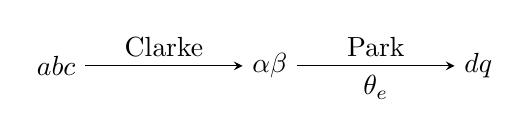
\begin{tikzpicture}[
    node distance=2cm,
    transform/.style={->, >=stealth}
]

\node (abc) {$abc$};
\node[right=of abc] (ab) {$\alpha\beta$};
\node[right=of ab] (dq) {$dq$};

\draw[transform] (abc) -- node[above] {Clarke} (ab);
\draw[transform] (ab) -- node[above] {Park}
                            node[below] {$\theta_e$} (dq);

\end{tikzpicture}
\end{center}

\begin{center}
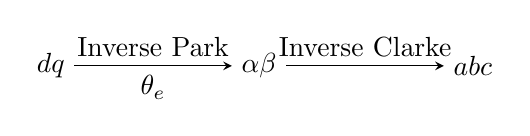
\begin{tikzpicture}[
    node distance=2cm,
    transform/.style={->, >=stealth}
]

\node (dq) {$dq$};
\node[right=of dq] (ab) {$\alpha\beta$};
\node[right=of ab] (abc) {$abc$};

\draw[transform] (dq) -- node[above] {Inverse Park}
                            node[below] {$\theta_e$} (ab);

\draw[transform] (ab) -- node[above] {Inverse Clarke} (abc);

\end{tikzpicture}
\end{center}


%=========================================================================%
\paragraph{Clarke Transformation}
%=========================================================================%


The forward and reverse reduced amplitude-invariant Clarke transforms respectively, are: 

\begin{equation}
    \begin{bmatrix}
        f_\alpha \\
        f_\beta
    \end{bmatrix}
    =
    \frac{2}{3}
    \begin{bmatrix}
        1 & -\frac{1}{2} & -\frac{1}{2} \\
        0 & \frac{\sqrt{3}}{2} & -\frac{\sqrt{3}}{2}
    \end{bmatrix}
    \begin{bmatrix}
        f_a \\
        f_b \\
        f_c
    \end{bmatrix}
\end{equation}

\begin{equation}
    \begin{bmatrix}
        f_a \\
        f_b \\
        f_c
    \end{bmatrix}
    =
    \begin{bmatrix}
        1 & 0 \\
        -\frac{1}{2} & \frac{\sqrt{3}}{2} \\
        -\frac{1}{2} & -\frac{\sqrt{3}}{2}
    \end{bmatrix}
    \begin{bmatrix}
        f_\alpha \\
        f_\beta
    \end{bmatrix}
\end{equation}


%=========================================================================%
\paragraph{Park Transformation}
%=========================================================================%


The forward and reverse reduced Park transforms respectively, are:

\begin{equation}
    \begin{bmatrix}
        f_d \\
        f_q
    \end{bmatrix}
    =
    \begin{bmatrix}
        \cos(\theta_e) & \sin(\theta_e) \\
        -\sin(\theta_e) & \cos(\theta_e)
    \end{bmatrix}
    \begin{bmatrix}
        f_\alpha \\
        f_\beta
    \end{bmatrix}
\end{equation}

\begin{equation}
    \begin{bmatrix}
        f_\alpha \\
        f_\beta
    \end{bmatrix}
    =
    \begin{bmatrix}
        \cos(\theta_e) & -\sin(\theta_e) \\
        \sin(\theta_e) & \cos(\theta_e)
    \end{bmatrix}
    \begin{bmatrix}
        f_d \\
        f_q
    \end{bmatrix}
\end{equation}


%=========================================================================%
\paragraph{Angle \& Speed Relationships}
%=========================================================================%

Electrical angle is related to mechanical (physical) angle by the number of pole pairs, $p$:

\begin{equation}
    \theta_e = p\theta_m
\end{equation}

Similarly:

\begin{equation}
    \omega_e = p\omega_m
\end{equation}

Then:

\begin{equation}
    \dot{\theta_e} = \frac{d\theta_e}{dt} = \omega_e
\end{equation}

And:

\begin{equation}
    \dot{\theta_m} = \frac{d\theta_m}{dt} = \omega_m
\end{equation}


%=========================================================================%
\subsubsection{Electrical Model}
%=========================================================================%


Starting with the machine flux linkages:

\begin{equation}
    \lambda_d = L_di_d + \lambda_m
\end{equation}

\begin{equation}
    \lambda_q = L_qi_q
\end{equation}

For a non-salient machine:

\begin{equation}
    L_d = L_q = L_\alpha = L_\beta = \frac{3}{2}L_s
\end{equation}

Then the final voltage model is:

\begin{equation}
    \boxed{
    v_d = R_si_d + L_d\frac{di_d}{dt} - \omega_eL_qi_q
    }
\end{equation}

\begin{equation}
    \boxed{
    v_q = R_si_q + L_q\frac{di_q}{dt} + \omega_eL_di_d + \omega_e\lambda_m
    }
\end{equation}

Rearranged into a form more practical for later sections:

\begin{equation}
    \boxed{
    \frac{di_d}{dt} = \frac{1}{L_d}(v_d - R_si_d + \omega_eL_qi_q)
    }
\end{equation}

\begin{equation}
    \boxed{
    \frac{di_q}{dt} = \frac{1}{L_q}(v_q - R_si_q - \omega_eL_di_d - \omega_e\lambda_m)
    }
\end{equation}

%=========================================================================%
\subsubsection{Electromagnetic Torque \& Mechanical Model}
%=========================================================================%

The general torque expression is:

\begin{equation}
    T_e = \frac{3}{2}p[\lambda_mi_q + (L_d - L_q)i_di_q]
\end{equation}

For the non-salient machines considered here, where the $d$- and $q$-axis inductances are equal:

\begin{equation}
    \boxed{
    T_e = \frac{3}{2}p\lambda_mi_q
    }
\end{equation}

The mechanical model is:

\begin{equation}
    \frac{d\omega_m}{dt} = \frac{1}{J}(T_e - T_L - B\omega_m)
\end{equation}


%=========================================================================%
\subsubsection{State-Space Model}
%=========================================================================%

The state vector is defined as as the vector containing the state variables: $i_d$, $i_q$, $\omega_m$, $\theta_m$. The input vector contains $v_d$, $v_q$, $T_L$. Then:

\begin{equation}
    \mathbf{x} =
    \begin{bmatrix}
        i_d \\
        i_q \\
        \omega_m \\
        \theta_m
    \end{bmatrix},
    \qquad
    \mathbf{u} =
    \begin{bmatrix}
        v_d \\
        v_q \\
        T_L
    \end{bmatrix}
\end{equation}

Then, the complete model is:

\begin{align}
    \dot{i_d} &= \frac{1}{L_d}(v_d - R_si_d + p\omega_mL_qi_q) \\[4pt]
    \dot{i_q} &= \frac{1}{L_q}(v_q - R_si_q - p\omega_mL_di_d - p\omega_m\lambda_m) \\[4pt]
    \dot{\omega_m} &= \frac{1}{J}\left[ \frac{3}{2}p\lambda_mi_q - T_L - B\omega_m\right] \\[4pt]
    \dot{\theta_m} &= \omega_m
\end{align}

The model developed in this chapter describes the response of the PMSM to an applied stator voltage vector. In practice, however, these continuous voltage commands cannot be applied directly to the motor. A motor drive is supplied by a DC source and must synthesize the required three-phase stator voltages through the discrete switching states of a three-phase voltage-source inverter. Chapter 2 therefore develops the relationship between the DC link voltage, inverter switching states, phase and line voltages, and the modulation techniques used to realize a command stator voltage vector. 


%=========================================================================%
\pagebreak
\section{Three-Phase Inverters \& Modulation Techniques}
\label{sec:three-phase-interters-and-modulation-techniques}


\subsection{Three-Phase Voltage Source Inverter}
\label{sec:three-phase-voltage-source-inverter}
%=========================================================================%

The model developed in Chapter 1 describes the response of a PMSM to a set of three phase stator voltages, $v_a$, $v_b$ and $v_c$. In practice, these voltages must be generated from the DC power source supplying the motor controller. A three-phase voltage source inverter (VSI) performs this conversion by switching the motor phase terminals between the DC-link rails. Through appropriate control of these switching states, the inverter can synthesize the three-phase voltage waveforms required to control the motor. 

A conventional two-level, three-phase VSI consists of three half-bridge switching legs connected in parallel across a DC link, as shown in Figure \ref{fig:3p-VSI}. Each inverter leg supplies one phase of the motor and consists of an upper and lower semiconducting switch. For the controller considered here, these switches may be implemented using MOSFETs, IGBTs or increasingly, GaNFETs or SiCFETs. However, the following analysis is independent of the switching device used.

%=========================================================================%

% Three phase inverter drawing

%=========================================================================%

\begin{figure}[H]
\begin{center}
\begin{circuitikz}[line width=0.8pt]

% ============================================================
% 3-Phase MOSFET Inverter
% ============================================================

\ctikzset{diodes/scale=0.35}
\ctikzset{tripoles/mos style/arrows}
\ctikzset{
    transistor bodydiode/scale=0.1,
    transistor bodydiode/color=black
}

% ============================================================
% MOSFETs
% ============================================================

% Phase A
\node[nigfete]
    (S1) at (0,3) {};
\node[right=16pt] at (S1.center) {$S_1$};

\node[nigfete]
    (S4) at (0,0) {};
\node[right=16pt] at (S4.center) {$S_4$};

% Phase B
\node[nigfete]
    (S2) at (4,3) {};
\node[right=16pt] at (S2.center) {$S_2$};

\node[nigfete]
    (S5) at (4,0) {};
\node[right=16pt] at (S5.center) {$S_5$};

% Phase C
\node[nigfete]
    (S3) at (8,3) {};
\node[right=16pt] at (S3.center) {$S_3$};

\node[nigfete]
    (S6) at (8,0) {};
\node[right=16pt] at (S6.center) {$S_6$};


% ============================================================
% BODY DIODES
% ============================================================

% Phase A

\draw
(S1.S)
node[circ] {}
-- ++(0.45,0)
to[D*] ($(S1.D)+(0.45,0)$)
-- (S1.D)
node[circ] {};

\draw
(S4.S)
node[circ] {}
-- ++(0.45,0)
to[D*] ($(S4.D)+(0.45,0)$)
-- (S4.D)
node[circ] {};


% Phase B

\draw
(S2.S)
node[circ] {}
-- ++(0.45,0)
to[D*] ($(S2.D)+(0.45,0)$)
-- (S2.D)
node[circ] {};

\draw
(S5.S)
node[circ] {}
-- ++(0.45,0)
to[D*] ($(S5.D)+(0.45,0)$)
-- (S5.D)
node[circ] {};


% Phase C

\draw
(S3.S)
node[circ] {}
-- ++(0.45,0)
to[D*] ($(S3.D)+(0.45,0)$)
-- (S3.D)
node[circ] {};

\draw
(S6.S)
node[circ] {}
-- ++(0.45,0)
to[D*] ($(S6.D)+(0.45,0)$)
-- (S6.D)
node[circ] {};


% ============================================================
% DC+ BUS
% ============================================================

\draw
(S1.D) -- ++(0,0.7)
coordinate (Aplus)
node[circ] {};

\draw
(S2.D) -- ++(0,0.7)
coordinate (Bplus)
node[circ] {};

\draw
(S3.D) -- ++(0,0.7)
coordinate (Cplus);

\draw
(Aplus) -- (Cplus);


% ============================================================
% SWITCH NODES / PHASE OUTPUTS
% ============================================================

% Phase A
\draw
(S1.S) -- (S4.D);

\coordinate (PhaseA) at ($(S1.S)!0.5!(S4.D)$);

\draw
(PhaseA)
node[circ] {}
-- ++(1.2,0)
node[right] {$V_{ag}$};


% Phase B
\draw
(S2.S) -- (S5.D);

\coordinate (PhaseB) at ($(S2.S)!0.5!(S5.D)$);

\draw
(PhaseB)
node[circ] {}
-- ++(1.2,0)
node[right] {$V_{bg}$};


% Phase C
\draw
(S3.S) -- (S6.D);

\coordinate (PhaseC) at ($(S3.S)!0.5!(S6.D)$);

\draw
(PhaseC)
node[circ] {}
-- ++(1.2,0)
node[right] {$V_{cg}$};


% ============================================================
% DC- BUS
% ============================================================

\draw
(S4.S) -- ++(0,-0.7)
coordinate (Agnd)
node[circ] {};

\draw
(S5.S) -- ++(0,-0.7)
coordinate (Bgnd)
node[circ] {};

\draw
(S6.S) -- ++(0,-0.7)
coordinate (Cgnd);

\draw
(Agnd) -- (Cgnd);


% ============================================================
% DC-LINK CAPACITOR
% ============================================================

\coordinate (DCtop) at ($(Aplus)+(-3.8,0)$);
\coordinate (DCbottom) at ($(Agnd)+(-3.8,0)$);

% Extend DC buses to capacitor
\draw
(Aplus) -- (DCtop);

\draw
(Agnd) -- (DCbottom);

% DC-link capacitor
\draw
(DCtop)
to[C]
(DCbottom);

% DC-link voltage label
\node[left, xshift=-16pt] at ($(DCtop)!0.5!(DCbottom)$)
{$V_{\mathrm{DC}}$};

% Polarity labels
\node[left] at ($(DCtop)!0.27!(DCbottom)$)
{$+$};

\node[left] at ($(DCtop)!0.73!(DCbottom)$)
{$-$};


% ============================================================
% GATE INPUTS
% ============================================================

% S1
\draw
(S1.G) -- ++(-1.35,0)
coordinate (S1gate);

\node[above] at ($(S1.G)!0.55!(S1gate)$)
{$G_1$};


% S4
\draw
(S4.G) -- ++(-1.35,0)
coordinate (S4gate);

\node[above] at ($(S4.G)!0.55!(S4gate)$)
{$G_4$};


% S2
\draw
(S2.G) -- ++(-1.35,0)
coordinate (S2gate);

\node[above] at ($(S2.G)!0.55!(S2gate)$)
{$G_2$};


% S5
\draw
(S5.G) -- ++(-1.35,0)
coordinate (S5gate);

\node[above] at ($(S5.G)!0.55!(S5gate)$)
{$G_5$};


% S3
\draw
(S3.G) -- ++(-1.35,0)
coordinate (S3gate);

\node[above] at ($(S3.G)!0.55!(S3gate)$)
{$G_3$};


% S6
\draw
(S6.G) -- ++(-1.35,0)
coordinate (S6gate);

\node[above] at ($(S6.G)!0.55!(S6gate)$)
{$G_6$};


\end{circuitikz}
\end{center}

\caption{Three-Phase Voltage Source Inverter Bridge}
\label{fig:3p-VSI}

\end{figure}

The ultimate objective of the inverter is to produce the desired stator currents within the motor through a process known as \textit{modulation}. However, the stator currents cannot be commanded directly by the inverter. Instead, the inverter applies voltages across the motor windings, which cause the currents to evolve according to the electrical dynamics of the machine. Therefore, the immediate objective of the modulation scheme is to synthesize the appropriate stator voltages required to produce the desired stator currents.

Each inverter leg can connect its corresponding phase terminal to either the positive or negative DC link rail. For phase $a$, turning on the upper switch, $S_1$ and turning off the lower switch, $S_4$ connects node $a$ to the the positive rail. Conversely, turning off $S_1$ and turning on $S_4$ connects node $a$ to the negative rail. Similar operation applies independently to phases $b$ and $c$.

It is important to differentiate the inverter node voltages, $v_{ag}$, $v_{bg}$ and $v_{cg}$ with the motor phase voltages. The inverter node voltages are referenced to ground, while the phase voltages are referenced to the motor neutral point. Further discussion will proceed in later sections on this topic. 

For the initial analysis, the semiconductor switches are assumed to be ideal. Consequently, a switch in the ON state has zero voltage drop, an OFF switch conducts no current, and switching transitions occur instantaneously. Non-ideal effects such as semiconductor voltage drop, switching delay, dead time, and minimum pulse width will be considered when practical implementation is discussed.


%=========================================================================%
\subsubsection{Inverter Switching Functions}
\label{sec:inverter-switching-functions}
%=========================================================================%


The switching state of each inverter leg can be represented by a binary switching function:

\[
    S_a, S_b, S_c \in \{0, 1\}
\]

The switching function for an arbitrary inverter leg with high side switch, $S_H$ and low side switch, $S_L$:

\[
S_n =
\begin{cases}
    1, & S_H \text{ ON, } S_L \text{ OFF}\\[4pt]
    0, & S_H \text{ OFF, } S_L \text{ ON}
\end{cases}
\]

The switching functions for $S_a$, $S_b$, $S_c$ are defined identically for their respective inverter legs. during normal operation, the high and low side switches must never be ON simultaneously. If both devices were ON, a direction conduction path would exist between the positive and negative power rails, constituting a short circuit scenario, otherwise called shoot through. This can produce a current great enough to destroy the switching devices.

In an ideal VSI, it is assumed one device is always conducting. Practical inverters introduce a short interval known as dead time between the turn off and and turn on of complementary switches in one leg. During this interval, neither switch is ON, and the resulting phase voltage depends on the direction of phase current and the available paths created by the FET body diodes. Initially, dead time will be neglected.

Under the ideal two state representation, the three swithcing functions can be collected into a switching state vector. 

\[
\mathbf{S} = 
\begin{bmatrix}
    S_a \\
    S_b \\
    S_c
\end{bmatrix}
\]

Because each of the three inverter legs can independently occupy one of two states, the three-phase inverter posses $2^3 = 8$ possible switching configurations:

\[
    000, 001, 010, 011, 100, 101, 110, 111
\]


%=========================================================================%
\subsection{Inverter Output Voltages}
\label{sec:inverter-output-voltages}
%=========================================================================%

%=========================================================================%
\subsubsection{Inverter Pole Voltages}
\label{sec:inverter-pole-voltages}
%=========================================================================%

We have just seen how by controlling the state of the inverter, we can independently control each inverter pole voltage through its switching function. Turning the high side FET ON connects the pole to $V_{DC}$, and turning the low side FET ON connects the pole to ground.

Using the eight inverter configurations and the switching function from Section \ref{sec:inverter-switching-functions}, we can completely determine the instantaneous voltages produced by an ideal two level inverter. The inverter pole voltages, with respect to ground are then:

\begin{equation}
    v_{ag} = S_aV_{DC}, \qquad
    v_{bg} = S_bV_{DC}, \qquad
    v_{cg} = S_cV_{DC}
\end{equation}

The set of possible instantaneous pole voltages is:

\[
    v_{xg} \in \{0, V_{DC}\}
\]


%=========================================================================%
\subsubsection{Phase Voltages}
\label{sec:phase-voltages}
%=========================================================================%

As alluded to earlier, it is important to distinguish between the inverter pole voltages, which are measured with respect to the inverter reference, and the motor phase voltages, which are measured with respect to the motor neutral point. For the wye-connected motor considered in this work, the neutral point \(n\) is floating and is not electrically connected to the inverter reference \(g\). Consequently, the potential of the motor neutral is floating, and varies according to the switching state of the inverter.

Figure \ref{fig:inverter-voltages} illustrates the relationship between the inverter pole voltages and the phase voltages of a wye connected motor. 

\begin{figure}[H]
    \centering
    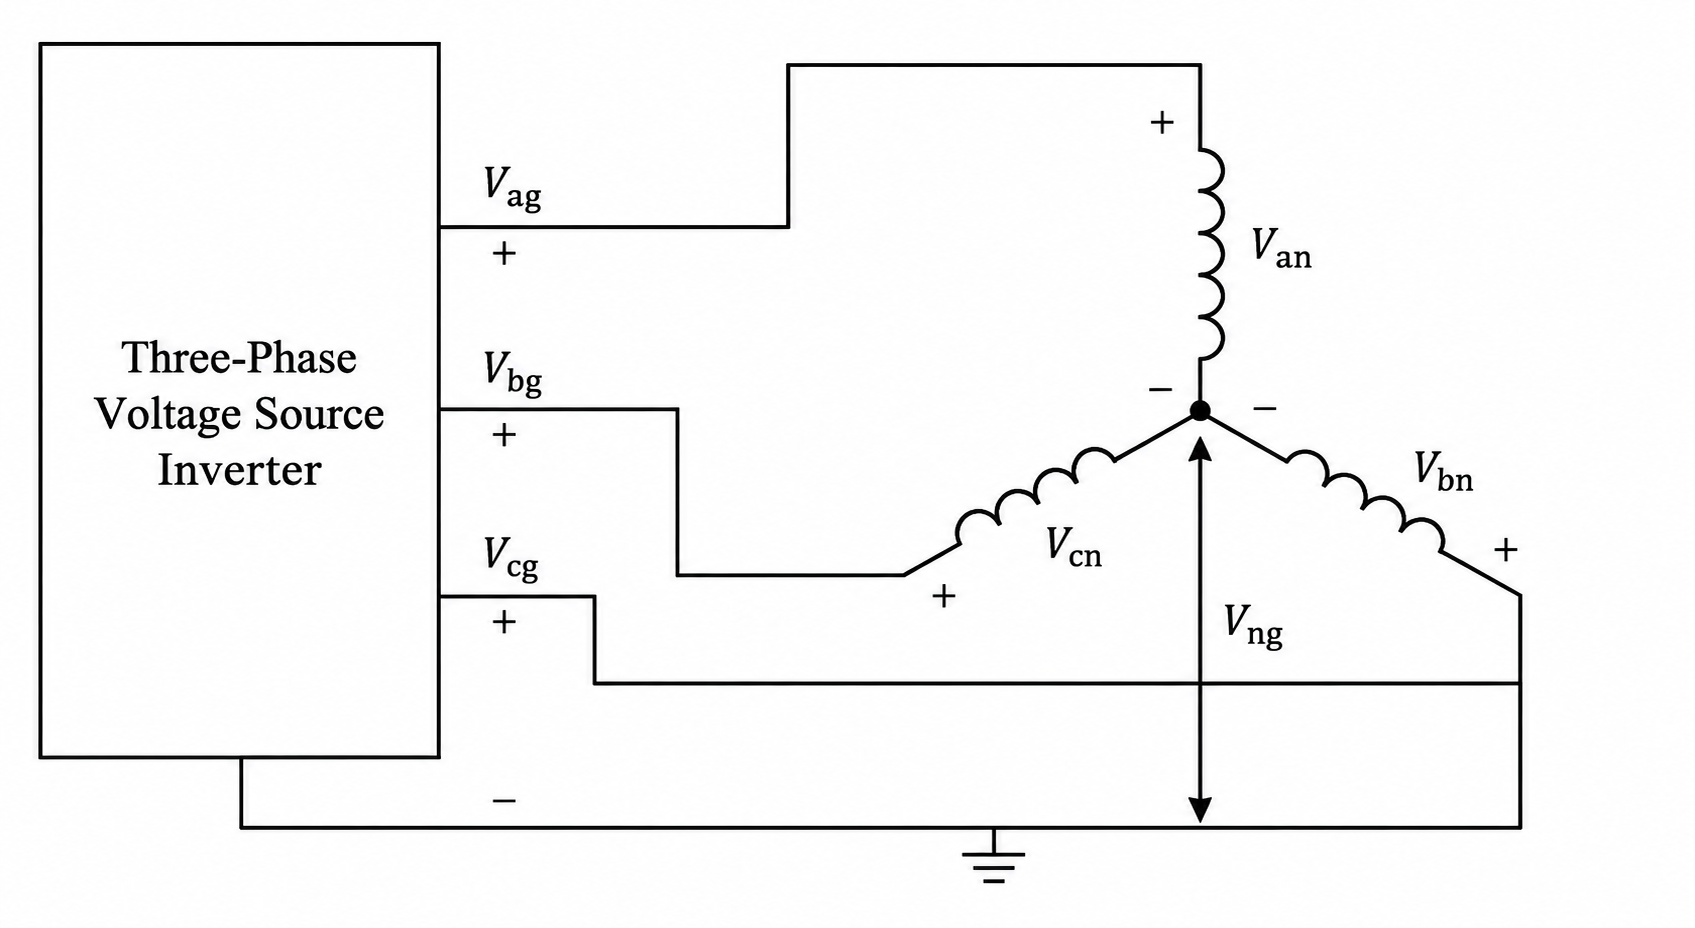
\includegraphics[width=0.6\linewidth]{inverter-voltages.png}
    \caption{Inverter Voltages}
    \label{fig:inverter-voltages}
\end{figure}

If we define the inverter pole voltages as:

\begin{equation}
    v_{ag} = v_a - v_g, \qquad
    v_{bg} = v_b - v_g, \qquad
    v_{cg} = v_c - v_g
\end{equation}

Where $v_a$, $v_b$ and $v_c$ are the potentials at the inverter nodes, and $v_g$ is the potential at the inverter ground or reference. The phase voltages are similarly defined as:

\begin{equation}
    v_{an} = v_a - v_n, \qquad
    v_{bn} = v_b - v_n, \qquad
    v_{cn} = v_c - v_n
\end{equation}

Lastly, we can also see that:

\begin{equation}
    v_{ng} = v_n - v_g
\end{equation}

Then, for example, given that:

\begin{equation}
    v_a = v_{ag} + v_g
\end{equation}

And:

\begin{equation}
    v_n = v_{ng} + v_g
\end{equation}

$v_{an}$ can be written as:

\begin{align}
    v_{an} 
    &= v_a - v_n \\
    &= v_{ag} + v_g - v_{ng} - v_g \\
    &= v_{ag} - v_{ng}
\end{align}

Which yields an additional expression for the phase voltages:

\begin{equation}
    v_{an} = v_{ag} - v_{ng}, \qquad
    v_{bn} = v_{bg} - v_{ng}, \qquad
    v_{cn} = v_{cg} - v_{ng}
\end{equation}

Or the inverter pole voltages:

\begin{equation}
    v_{ag} = v_{an} + v_{ng}, \qquad
    v_{bg} = v_{bn} + v_{ng}, \qquad
    v_{cg} = v_{cn} + v_{ng}
\end{equation}

If we take the sum of the inverter pole voltages:

\begin{equation}
    v_{ag} + v_{bg} + v_{cg} = v_{an} + v_{bn} + v_{cn} + 3v_{ng}
\end{equation}

Rearranging for $v_{ng}$:

\begin{equation}
\label{eqn-v-ng}
    v_{ng} = \frac{1}{3}(v_{ag} + v_{bg} + v_{cg}) - \frac{1}{3}(v_{an} + v_{bn} + v_{cn})
\end{equation}

Where second term, called the zero-sequence component, is defined as:

\begin{equation}
    v_0 = \frac{1}{3}(v_{an} + v_{bn} + v_{cn})
\end{equation}

Exactly as shown as in the Clarke transform. For a wye connected motor, it is easy to see from a KCL that the sum of phase currents is zero. It is somewhat less trivial to show that:

\begin{equation}
    v_{an} + v_{bn} + v_{cn} = 0
\end{equation}

We briefly do so here, beginning with the phase voltage equations from Section \ref{sec:abc-frame}:

\begin{equation}
    v_{an} = R_si_a + L_s\frac{di_a}{dt} + L_m\frac{di_b}{dt} + L_m\frac{di_c}{dt} + e_a
\end{equation}

\begin{equation}
    v_{bn} = R_si_b + L_m\frac{di_a}{dt} + L_s\frac{di_b}{dt} + L_m\frac{di_c}{dt} + e_b
\end{equation}

\begin{equation}
    v_{cn} = R_si_c + L_m\frac{di_a}{dt} + L_m\frac{di_b}{dt} + L_s\frac{di_c}{dt} + e_c
\end{equation}

Taking their sum yields:

\begin{align}
    v_{an} + v_{bn} + v_{cn} &= R_s(i_a + i_b + i_c) + L_s\frac{d}{dt}(i_a + i_b + i_c) + 2L_m\frac{d}{dt}(i_a + i_b + i_c) + e_a + e_b + e_c
\end{align}

By definition of Kichoff's Current Law (KCL), the sum of currents entering and leaving a node must be equal to zero. Therefore, at the neutral point:

\begin{equation}
    i_a + i_b + i_c = 0
\end{equation}

Also recall from Section \ref{sec:winding-inductances} that for an ideal, sinusoidal PMSM, the back-EMF is also three phase and sinusoidal, which we know sums to zero. Hence:

\begin{equation}
    e_a + e_b + e_c = 0
\end{equation}

And we have that for a balanced, three phase, sinusoidal PMSM, the sum of phase voltages, and therefore the zero-sequence voltage, is zero. Using this result with Equation \ref{eqn-v-ng}, we find that:

\begin{equation}
    v_{ng} = \frac{1}{3}(v_{ag} + v_{bg} + v_{cg})
\end{equation}

Now that we have an expression for the neutral voltage in terms of the inverter pole voltages, we can solve for the phase voltages exclusively in terms of the inverter pole voltages. From earlier:

\begin{equation}
    v_{an} = v_{ag} - v_{ng}, \qquad
    v_{bn} = v_{bg} - v_{ng}, \qquad
    v_{cn} = v_{cg} - v_{ng}
\end{equation}

Substituting the equation for $v_{ng}$:

\begin{align}
    v_{an} &= v_{ag} - \frac{1}{3}(v_{ag} + v_{bg} + v_{cg}) \\
    &= \frac{2}{3}v_{ag} - \frac{1}{3}v_{bg} - \frac{1}{3}v_{cg}
\end{align}

\begin{align}
    v_{bn} &= v_{bg} - \frac{1}{3}(v_{ag} + v_{bg} + v_{cg}) \\
    &= - \frac{1}{3}v_{ag} + \frac{2}{3}v_{bg} - \frac{1}{3}v_{cg}
\end{align}

\begin{align}
    v_{cn} &= v_{cg} - \frac{1}{3}(v_{ag} + v_{bg} + v_{cg}) \\
    &= - \frac{1}{3}v_{ag} - \frac{1}{3}v_{bg} + \frac{2}{3}v_{cg}
\end{align}

In matrix form, this becomes:

\begin{equation}
    \begin{bmatrix}
        v_{an} \\
        v_{bn} \\
        v_{cn}
    \end{bmatrix}
    = \frac{1}{3}
    \begin{bmatrix}
        2 & -1 & -1 \\
        -1 & 2 & -1 \\
        -1 & -1 & 2 \\
    \end{bmatrix}
    \begin{bmatrix}
        v_{ag} \\
        v_{bg} \\
        v_{cg}
    \end{bmatrix}
\end{equation}

If we combine this with the switching functions: 

\begin{equation}
    v_{ag} = S_aV_{DC}, \qquad
    v_{bg} = S_bV_{DC}, \qquad
    v_{cg} = S_cV_{DC}
\end{equation}

We find that:

\begin{equation}
    v_{an} = \frac{V_{DC}}{3}(2S_a - S_b - S_c), \qquad
    v_{bn} = \frac{V_{DC}}{3}(-S_a + 2S_b - S_c), \qquad
    v_{cn} = \frac{V_{DC}}{3}(-S_a - S_b + 2S_c)
\end{equation}

In matrix form:

\begin{equation}
    \begin{bmatrix}
        v_{an} \\
        v_{bn} \\
        v_{cn}
    \end{bmatrix}
    = \frac{V_{DC}}{3}
    \begin{bmatrix}
        2 & -1 & -1 \\
        -1 & 2 & -1 \\
        -1 & -1 & 2 \\
    \end{bmatrix}
    \begin{bmatrix}
        S_a \\
        S_b \\
        S_c
    \end{bmatrix}
\end{equation}

Notice that the maximum \textit{instantaneous} phase voltage magnitude for a given state is $2V_{DC}/3$. The set of possible instantaneous phase voltages is:

\[
    v_{xn} \in \biggl\{ -\frac{2V_{DC}}{3}, -\frac{V_{DC}}{3}, 0, \frac{V_{DC}}{3}, \frac{2V_{DC}}{3} \biggr\}
\]


%=========================================================================%
\subsubsection{Line Voltages}
\label{sec:line-voltages}
%=========================================================================%

In addition to the phase-to-neutral voltages, the output of a three-phase inverter can be described using the line-to-line voltages. A line-to-line voltage represents the potential difference between two motor phase terminals. The three line-to-line voltages are defined as:

\begin{equation}
    v_{ab} = v_{an} - v_{bn}, \qquad
    v_{bc} = v_{bn} - v_{cn}, \qquad
    v_{ca} = v_{cn} - v_{an}
\end{equation}

Or, since the neutral voltage cancels out:

\begin{equation}
    v_{ab} = v_{a} - v_{b}, \qquad
    v_{bc} = v_{b} - v_{c}, \qquad
    v_{ca} = v_{c} - v_{a}
\end{equation}

We can also see from:

\begin{equation}
    v_{an} = v_{ag} - v_{ng}
\end{equation}

And:

\begin{equation}
    v_{bn} = v_{bg} - v_{ng}
\end{equation}

That:

\begin{align}
    v_{ab} &= v_{an} - v_{bn} \\
    &= v_{ag} - v_{ng} - v_{bg} + v_{ng} \\
    &= v_{ag} - v_{bg}
\end{align}

Hence we have:

\begin{equation}
    v_{ab} = v_{ag} - v_{bg}, \qquad
    v_{bc} = v_{bg} - v_{cg}, \qquad
    v_{ca} = v_{cg} - v_{ag}
\end{equation}

Notice that the neutral point voltage, $v_{ng}$, cancels from each expression. Consequently, the line-to-line voltages are independent of the instantaneous potential of the floating motor neutral. Substituting the inverter pole voltage for the switching functions:

\begin{equation}
    v_{ab} = V_{DC}(S_a - S_b), \qquad
    v_{bc} = V_{DC}(S_b - S_c), \qquad
    v_{ca} = V_{DC}(S_c - S_a)
\end{equation}

In matrix form:

\begin{equation}
    \begin{bmatrix}
        v_{ab} \\
        v_{bc} \\
        v_{ca}
    \end{bmatrix}
    = V_{DC}
    \begin{bmatrix}
        1 & -1 & 0 \\
        0 & 1 & -1 \\
        -1 & 0 & 1
    \end{bmatrix}
    \begin{bmatrix}
        S_a \\
        S_b \\
        S_c
    \end{bmatrix}
\end{equation}

Since the line voltages are proportional to the difference of switch states, each instantaneous line voltage can only assume three possible values:

\[
    v_{xy} \in \{-V_{DC}, 0, V_{DC}\}
\]

Lastly, note that by definition, the sum of line voltages is always zero, regardless of balance:

\begin{equation}
    v_{ab} + v_{bc} + v_{ca} = (v_a - v_b) + (v_b - v_c) + (v_c - v_a) = 0
\end{equation}

Hence:

\begin{equation}
    v_{ab} + v_{bc} + v_{ca} = 0
\end{equation}


%=========================================================================%
\subsection{Inverter Switching States \& Space Vectors}
\label{sec:inverter-switching-states-and-space-vectors}
%=========================================================================%

Using all eight switching states from Section \ref{sec:inverter-switching-functions}, and the matrix relating the phase voltages to the switch states in Section \ref{sec:phase-voltages}, we can evaluate the phase voltages for all states:

\[
    \{S_a, S_b, S_c\} \in \{000, 001, 010, 011, 100, 101, 110, 111\}
\]

\begin{equation}
    \begin{bmatrix}
        v_{an} \\
        v_{bn} \\
        v_{cn}
    \end{bmatrix}
    = \frac{V_{DC}}{3}
    \begin{bmatrix}
        2 & -1 & -1 \\
        -1 & 2 & -1 \\
        -1 & -1 & 2 \\
    \end{bmatrix}
    \begin{bmatrix}
        S_a \\
        S_b \\
        S_c
    \end{bmatrix}
\end{equation}

Summarizing the result in table form:

\begin{table}[H]
    \centering
    \caption{Three-Phase Inverter Switching States and Phase Voltages}
    \label{tab:inverter_switching_states}

    % Table spacing
    \renewcommand{\arraystretch}{2.3}
    \setlength{\tabcolsep}{14pt}

    \begin{tabular}{c c c c c}
        \hline
        \textbf{Vector} &
        $\boldsymbol{S_aS_bS_c}$ &
        $\boldsymbol{v_{an}}$ &
        $\boldsymbol{v_{bn}}$ &
        $\boldsymbol{v_{cn}}$ \\
        \hline

        $\mathbf{V}_0$ & $000$
        & $0$ & $0$ & $0$ \\

        $\mathbf{V}_1$ & $100$
        & $\dfrac{2V_{DC}}{3}$
        & $-\dfrac{V_{DC}}{3}$
        & $-\dfrac{V_{DC}}{3}$ \\

        $\mathbf{V}_2$ & $110$
        & $\dfrac{V_{DC}}{3}$
        & $\dfrac{V_{DC}}{3}$
        & $-\dfrac{2V_{DC}}{3}$ \\

        $\mathbf{V}_3$ & $010$
        & $-\dfrac{V_{DC}}{3}$
        & $\dfrac{2V_{DC}}{3}$
        & $-\dfrac{V_{DC}}{3}$ \\

        $\mathbf{V}_4$ & $011$
        & $-\dfrac{2V_{DC}}{3}$
        & $\dfrac{V_{DC}}{3}$
        & $\dfrac{V_{DC}}{3}$ \\

        $\mathbf{V}_5$ & $001$
        & $-\dfrac{V_{DC}}{3}$
        & $-\dfrac{V_{DC}}{3}$
        & $\dfrac{2V_{DC}}{3}$ \\

        $\mathbf{V}_6$ & $101$
        & $\dfrac{V_{DC}}{3}$
        & $-\dfrac{2V_{DC}}{3}$
        & $\dfrac{V_{DC}}{3}$ \\

        $\mathbf{V}_7$ & $111$
        & $0$ & $0$ & $0$ \\

        \hline
    \end{tabular}
\end{table}

We could perform vector addition using the given magnitudes and each vector direction as given by the space vector diagram in Figure \ref{fig:abc-phasors}, however, it may be more simple to convert to $\alpha\beta$ frame using the Clarke transform first. Doing so yields the following table:

\begin{table}[H]
    \centering
    \caption{Inverter Voltage Space Vectors in the $\alpha\beta$ Frame}
    \label{tab:inverter_space_vectors}

    \renewcommand{\arraystretch}{2.3}
    \setlength{\tabcolsep}{12pt}

    \begin{tabular}{c c c c c c}
        \hline
        \textbf{Vector} &
        $\boldsymbol{S_aS_bS_c}$ &
        $\boldsymbol{v_\alpha}$ &
        $\boldsymbol{v_\beta}$ &
        $\boldsymbol{|\mathbf{V}_k|}$ &
        $\boldsymbol{\theta_k}$ \\
        \hline

        $\mathbf{V}_0$ & $000$
        & $0$
        & $0$
        & $0$
        & -- \\

        $\mathbf{V}_1$ & $100$
        & $\dfrac{2V_{DC}}{3}$
        & $0$
        & $\dfrac{2V_{DC}}{3}$
        & $0^\circ$ \\

        $\mathbf{V}_2$ & $110$
        & $\dfrac{V_{DC}}{3}$
        & $\dfrac{V_{DC}}{\sqrt{3}}$
        & $\dfrac{2V_{DC}}{3}$
        & $60^\circ$ \\

        $\mathbf{V}_3$ & $010$
        & $-\dfrac{V_{DC}}{3}$
        & $\dfrac{V_{DC}}{\sqrt{3}}$
        & $\dfrac{2V_{DC}}{3}$
        & $120^\circ$ \\

        $\mathbf{V}_4$ & $011$
        & $-\dfrac{2V_{DC}}{3}$
        & $0$
        & $\dfrac{2V_{DC}}{3}$
        & $180^\circ$ \\

        $\mathbf{V}_5$ & $001$
        & $-\dfrac{V_{DC}}{3}$
        & $-\dfrac{V_{DC}}{\sqrt{3}}$
        & $\dfrac{2V_{DC}}{3}$
        & $240^\circ$ \\

        $\mathbf{V}_6$ & $101$
        & $\dfrac{V_{DC}}{3}$
        & $-\dfrac{V_{DC}}{\sqrt{3}}$
        & $\dfrac{2V_{DC}}{3}$
        & $300^\circ$ \\

        $\mathbf{V}_7$ & $111$
        & $0$
        & $0$
        & $0$
        & -- \\

        \hline
    \end{tabular}
\end{table}

Plotting all eight vectors yields the space vector diagram for a two-level, three-phase inverter, shown in Figure \ref{fig:space-vector-diagram}. Notice that all six active switching vectors (neglecting the zero vectors at the origin) have equal magnitudes of:

\begin{equation}
    |\mathbf{v}_k| = \sqrt{v_\alpha^2 + v_\beta^2} = \frac{2V_{DC}}{3}
\end{equation}

\begin{figure}[H]
    \centering
    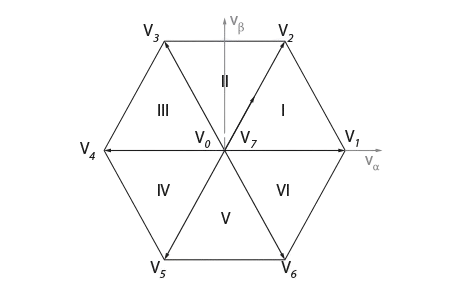
\includegraphics[width=0.5\linewidth]{space-vector-diagram.png}
    \caption{Space Vector Diagram}
    \label{fig:space-vector-diagram}
\end{figure}

Table \ref{tab:inverter_space_vectors} and Figure \ref{fig:space-vector-diagram} summarize the complete set of states that the inverter considered in this discussion can produce. The central idea of a space vector is that a single, two-dimensional vector can be used to represent the instantaneous state of a balanced three-phase quantity. Instead of thinking about separate instantaneous voltages:

\begin{equation}
    v_a(t), \qquad
    v_b(t), \qquad
    v_c(t)
\end{equation}

We represent the same information using a single vector in the stationary $\alpha\beta$ plane:

\begin{equation}
    \mathbf{v}_s(t) = v_\alpha(t)\hat{\alpha} + v_\beta(t)\hat{\beta}
\end{equation}

The difference between the discussion here and that of Section \ref{sec:alpha-beta-frame} and the Clarke transform, is that while the $\alpha\beta$ frame provides a general reference frame to express three-phase quantities, here, we restrict ourselves to the vectors that we are physically able to produce using hardware.

The other important identification to make is that term \textit{space vector} originates from the fact that the phase (electrical angle) of the space vector corresponds to the mechanical angle of the rotor, related by the number of pole pairs. The three motor phases are distributed in space around the stator, separated electrically by $120^\circ$. Each phase winding therefore corresponds to a particular spatial axis:

\begin{equation}
    a \rightarrow 0^\circ, \qquad
    b \rightarrow 120^\circ, \qquad
    c \rightarrow 240^\circ
\end{equation}

Contributions from all three phase axis can then be combined into a single resultant vector in the stator plane. Using the amplitude invariant convention, this is commonly written as:

\begin{equation}
    \mathbf{v}_s = \frac{2}{3}(v_a + v_be^{j2\pi/3} + v_ce^{-j2\pi/3})
\end{equation}

Where the complex exponential's encode the spatial orientations of the $b$ and $c$ axis. Expanding:

\begin{equation}
    e^{j2\pi/3} = -\frac{1}{2} + j\frac{\sqrt{3}}{2}, \qquad
    e^{-j2\pi/3} = -\frac{1}{2} - j\frac{\sqrt{3}}{2}
\end{equation}

Which gives:

\begin{align}
    \mathbf{v}_s &= \frac{2}{3}\left[(v_a - \frac{1}{2}v_b - \frac{1}{2}v_c + j\frac{\sqrt{3}}{2}(v_b - v_c) \right] \\
    &= v_\alpha + jv_\beta
\end{align}

With:

\begin{align}
    v_\alpha = \frac{2}{3}\left(v_a -\frac{1}{2}v_b - \frac{1}{2}v_c \right) \\[6pt]
    v_\beta = \frac{2}{3}\left(\frac{\sqrt{3}}{2}v_b - \frac{\sqrt{3}}{2}v_c \right)
\end{align}

Which is exactly the Clarke transform we have derived previously. Recall that for a positive-sequence three-phase system, the phase quantities are represented as \(a=\cos(\omega t)\), \(b=\cos(\omega t-120^\circ)\), and \(c=\cos(\omega t-240^\circ)\). These angular offsets represent \textit{temporal phase shifts} (i.e shifts in time) and should not be confused with the physical orientation of the phase axes. Spatially, the corresponding phase axes are positioned at \(0^\circ\), \(+120^\circ\), and \(+240^\circ\), respectively. The opposite signs of the temporal and spatial phase displacements are what allows a field that rotates in the positive spatial direction.

In other words, the temporal phase values shift each phase in the positive sequence to be later in time than the last. This is described by an increasingly negative phase angle. Conversely, since a CCW rotation is taken as positive rotation in the space vector plane, increasingly spatially delayed axes are specified by increasingly positive angles. 


%=========================================================================%
\subsection{Pulse-Width Modulation}
\label{sec:pulse-width-modulation}
%=========================================================================%

Section \ref{sec:inverter-switching-states-and-space-vectors} established that a two-level three-phase inverter can produce only a finite set of instantaneous output voltages. The motor model developed in Chapter \ref{sec:mathematical-model-of-pmsms}, however, describes the machine in terms of continuously varying stator voltages. Pulse-width modulation (PWM) provides the connection between these two descriptions.

Rather than attempting to produce a desired voltage instantaneously, PWM rapidly switches between the available inverter states such that the average voltage over a switching period approaches the desired voltage. If the switching period is sufficiently short relative to the electrical dynmics of the motor, the stator inductance limits the resulting high-frequency current ripply and the motor responds primarily to the lower frequency average voltage.

Each inverter legs consists of an upper and lower switching device which are operated complementarily. In otherwords, while one is in the ON state, the other is in the OFF state and vice versa. The PWM signal generated for a given phase may therefore be used to command the upper switching device, while its complement commands the lower device.

%=========================================================================%
\subsubsection{Fast Averaged Signals}
\label{sec:fast-averaged-signals}
%=========================================================================%

Considere the inverter leg circuit of phase-$a$, consisting of the upper and lower MOSFETs. The switching period of a PWM signal is defined as:

\begin{equation}
    T_s = \frac{1}{f_s}
\end{equation}

Where $f_s$ is the switching frequency. If phase-$a$ has its upper switch ON for a duration of $T_a$ during each switching period $T_s$, the duty cycle of the phase-$a$ inverter leg is defined as the ratio of the duration where the pulse is ON to the total period:

\begin{equation}
    D_a = \frac{T_a}{T_s}, \qquad
    0 \leq D_a \leq 1
\end{equation}

Recall from Section \ref{sec:inverter-switching-functions} that the instantaneous phase-$a$ pole voltage is:

\begin{equation}
    v_{ag} = S_aV_{DC}, \qquad
    S_a \in \{0, 1\}
\end{equation}

The average pole voltage over one switching period is therefore:

\begin{equation}
    \overline{v}_{ag} = \frac{1}{T_s}\int_0^{T_s} v_{ag}(t)dt
\end{equation}

Since $v_{ag} = V_{DC}$ for a fraction $D_a$ of the switching period and $v_{ag} = 0$ for the remaining $1 - D_a$ fraction:

\begin{align}
    \overline{v}_{ag} 
    &= \frac{1}{T_s}\int_0^{D_aT_s} V_{DC}dt \\[4pt]
    &= \frac{1}{T_s}[V_{DC}(D_aT_s) - 0] \\[4pt]
    &= D_aV_{DC}
\label{eqn:average-voltage}
\end{align}

And therefore:

\begin{equation}
    \overline{v}_{ag} = D_aV_{DC}, \qquad
    \overline{v}_{bg} = D_bV_{DC}, \qquad
    \overline{v}_{cg} = D_cV_{DC}
\end{equation}

Thus, although each inverter pole voltage can instantaneously assume only the values $0$ and $V_{DC}$, its average value may be continuously controlled between these limits by varying its duty cycle. This is known as a fast averaged signal. Note that duty cycle must be a value between $0$ and $1$. Then if $D = 0$, the output is connected to the source 0\% of the time, and the output voltage is zero. Conversely, if $D = 1$, the output is connected to the source 100\% of the time, and the output voltage is equal to $V_{DC}$.


%=========================================================================%
\subsubsection{PWM Signal Generation}
%=========================================================================%

We have established that a PWM waveform can be described in terms of the duty cycle and DC-link rail voltages required to produce a desired switching-period average voltage. Practically speaking, a PWM signal may be generated by comparing a reference sigal with a periodic carrier signal. The carrier is typically a triangular or sawtooth waveform whose period, $T_s$, determins the PWM switching period. 

Let $v_{ref}(t)$ dentoes the reference signal and $v_{car}(t)$ the carrier signal. The switching function may be defined by the compartor function:

\begin{equation}
    S(t) =
    \begin{cases}
        1, & v_{ref}(t) \geq v_{car}(t) \\
        0, & v_{ref}(t) < v_{car}(t)
    \end{cases}    
\end{equation}

The intersections between the reference and the carrier waveforms determine the swtiching instants. Consequently, changing the magnitude of the reference signal changes the fraction of each switching period for which $S(t) = 1$, thereby controlling the duty cycle. We can see this in Figure \ref{fig:pwm-generation-sawtooth}, where the duty cycle is derived below. For a DC siganl and rising sawtooth, respectiely:

\begin{equation}
    v_{ref}(t) = D, \qquad
    0 \leq D \leq 1
\end{equation}

\begin{equation}
    v_{car}(t) = \frac{t}{T_s}, \qquad
    0 \leq t < T_s
\end{equation}

The switching transition occurs when both signals are equal, at the time $t_{on}$:

\begin{equation}
    v_{ref}(t) = v_{car}(t)
\end{equation}

Therefore:

\begin{equation}
\label{eqn:duty-cycle}
    D = \frac{t_{on}}{T_s}
\end{equation}

Which is the exact result we found in Section \ref{sec:fast-averaged-signals}. Therefore, for a normalized carrier and reference, the amplitude of the reference signal becomes the proportion of the sawtooth period where the pulse is on. In other words, the amplitude of the reference is approxiamtely equal to the duty cycle.

\begin{figure}[H]
    \centering
    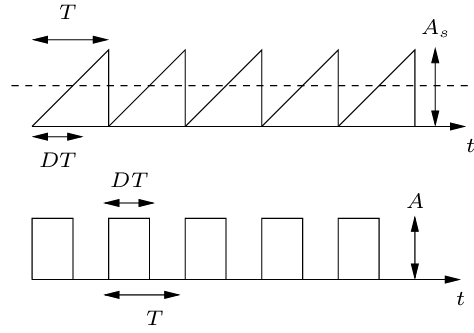
\includegraphics[width=0.5\linewidth]{pwm-generation-sawtooth.png}
    \caption{PWM Generation Using a Sawtooth Carrier and DC Reference}
    \label{fig:pwm-generation-sawtooth}
\end{figure}

This is known as edge-aligned PWM since the edges of the sawtooth correspond to the edges of the pulse. More commonly used is center aligned PWM, where a triangular wave is used instead of a sawtooth carrier. This results in PWM signals that are symmetric about the carrier, as shown in Figure \ref{fig:center-aligned-pwm}, with a duty cycle as given by Equation \ref{eqn:duty-cycle}.

\begin{figure}[H]
    \centering
    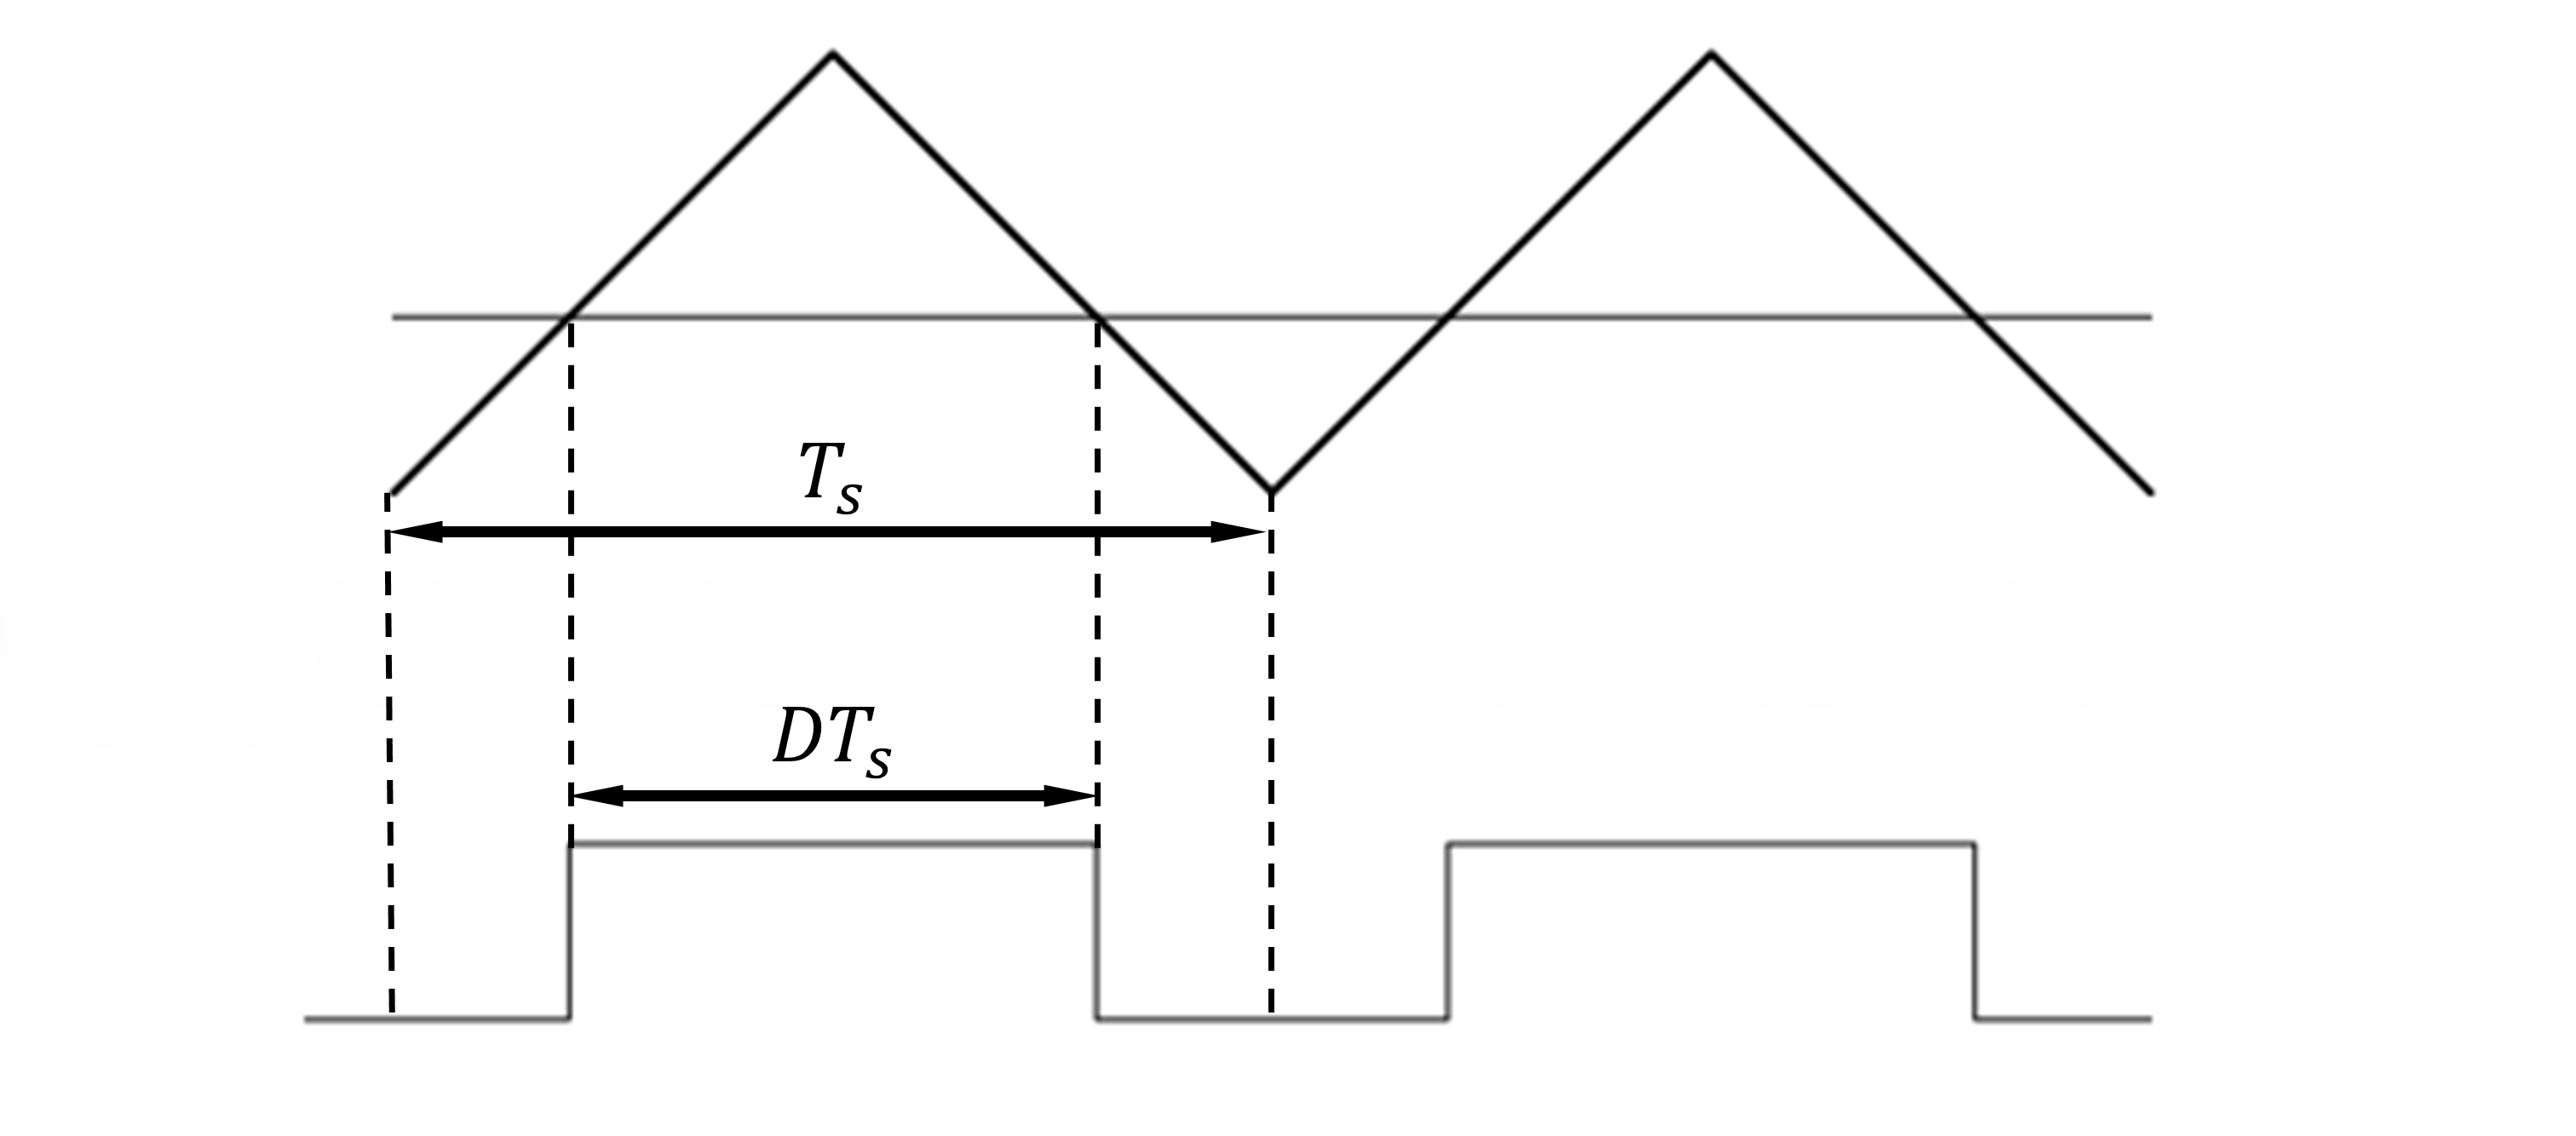
\includegraphics[width=0.65\linewidth]{center-aligned-pwm.png}
    \caption{Center Aligned PWM}
    \label{fig:center-aligned-pwm}
\end{figure}

We will later explore the benefits of center aligned PWM over edge aligned PWM, including lower EMI and noise, better harmonic performance and easier ADC sampling. The above examples consider a constant DC reference signal, resulting in a PWM waveform with a constant duty cycle. More generally, the reference signal may vary with time. If the switching frequency is sufficiently high relative to the rate of change of the reference ($f_r << f_c$), the reference can be considered approximately constant over each individual switching period. 

Consequently, the duty cycle during each period is determined by the instantaneous value of the reference signal. For a carrier normalized between 0 and 1:

\begin{equation}
    D(t) \approx v_{ref}(t), \qquad
    0 \leq v_{ref}(t) \leq 1
\end{equation}

The resulting PWM waveform therefore has a time-varying duty cycle which encodes the shape of the reference signal. Although the instantaneous PWM output is binary, its average value of each switching period follows the reference. This is illustrated in Figure \ref{fig:pwm-generation}, although for a system in which the carrier, reference, and corresponding PWM signal vary between $-1$ and $1$. 

\begin{figure}[H]
    \centering
    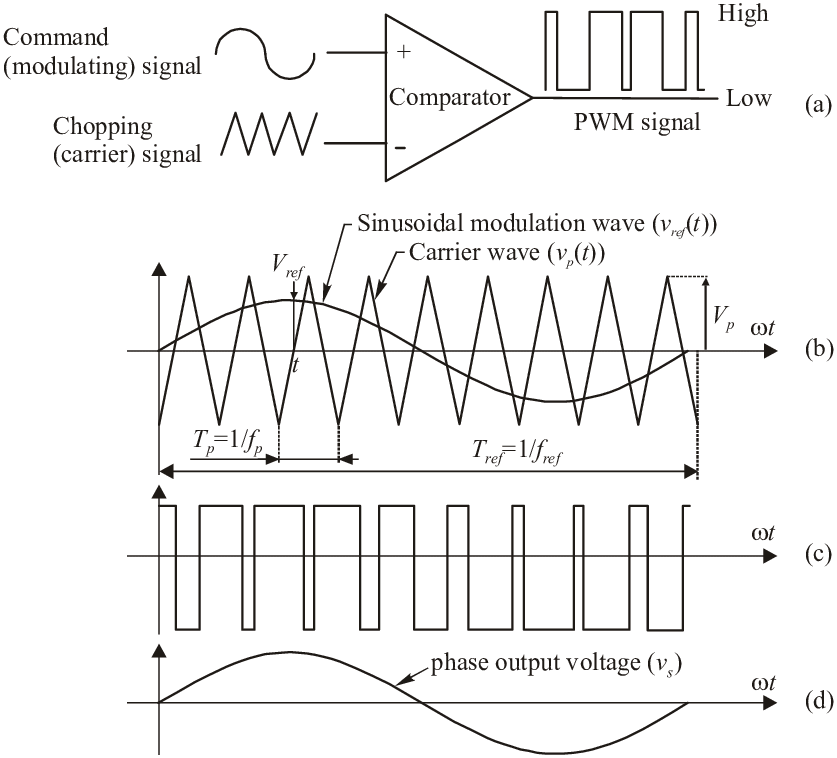
\includegraphics[width=0.5\linewidth]{pwm-generation.png}
    \caption{Center Aligned PWM}
    \label{fig:pwm-generation}
\end{figure}

A sinusoidal phase voltage such as that in Figure \ref{fig:pwm-generation} would require an inverter leg with a bipolar supply ($-V_{DC}, V_{DC}$). However, we can also produce a PWM signal corresponding to a sinusoidal reference for an inverter switching between $V_{DC}$ and ground. Consider the reference signal, $v_{ref}(t)$:

\begin{equation}
    v_{ref}(t) = \frac{1}{2} + \frac{m}{2}\sin(\omega t), \qquad
    0 \leq m \leq 1, \qquad
    0 \leq v_{ref}(t) \leq 1
\end{equation}

Then:

\begin{equation}
    D(t) = \frac{1}{2} + \frac{m}{2}\sin(\omega t)
\end{equation}

If PWM switches between $0$ and $V_{DC}$, from Equation \ref{eqn:average-voltage}:

\begin{equation}
    \overline{v}_{PWM}(t) \approx V_{DC} \left[ \frac{1}{2} + \frac{m}{2}\sin(\omega t) \right]
\end{equation}

It is important to note that the PWM waveform does not resemble the reference waveform instantaneously. Rather, information about the reference is contained in the changing pulse widths. When considered on a time scale much longer than the period, the local average of the PWM waveoform follows the reference.

This principle can be extended to three-phase voltage source inverters by using three sinusoidal reference signals displaced by $120^\circ$. Comparing each reference with a common high-frequency carrier produces the switching commands for the three inverter legs. We will soon explore this technique, known as sinusoidal pulse-width modulation.


%=========================================================================%
\subsubsection{Fast Switching Appoximation}
%=========================================================================%

The average voltage introduced in the preceding section does not imply that the inverter physically produces a continous voltgae equal to $\overline{v}$. At every instant, the inverter remains in one of its discrete switching states. Rather, the average voltage represetnation describes the effect of rapidly switched voltage on the comparatively slow electrical dynmics of the motor.

To illustrate this, consider a simplified single-phase inductive load described by:

\begin{equation}
    v(t) = Ri(t) + L\frac{di(t)}{dt} + e(t)
\end{equation}

Where $R$ and $L$ represent the winding resistance and inductance, respectively, and e(t) represents the back-EMF. Rearranging for rate of change of current gives:

\begin{equation}
    \frac{di(t)}{dt} = \frac{1}{L}[v(t) - Ri(t) - e(t)]
\end{equation}

Integrating over one switching period, $T_s$, gives the change in current:

\begin{equation}
    i(t_0 + T_s) - i(t_0) = \frac{1}{L} \int_{t_0}^{t_0 + T_s} [v(t) - Ri(t) - e(t)] dt
\end{equation}

Defining:

\begin{equation}
    \Delta i = i(t_0 + T_s) - i(t_0)
\end{equation}

We obtain:

\begin{equation}
    \Delta i = \frac{1}{L} \left[ \int_{t_0}^{t_0 + T_s} v(t) dt + \int_{t_0}^{t_0 + T_s} Ri(t) dt + \int_{t_0}^{t_0 + T_s} e(t) dt \right]
\end{equation}

If the switching period is sufficently short relative to the electrical and mechancial dynamics of the motor, the current and back-EMF vary only slightly during a single switching period. They may therefore be appoximated as constant over $T_s$:

\begin{equation}
    i(t) \approx i(t_0), \qquad
    e(t) \approx e(t_0)
\end{equation}

Consequently:

\begin{equation}
    \Delta i \approx \frac{1}{L} \left[ \int_{t_0}^{t_0 + T_s} v(t) dt - T_sRi(t_0) - T_se(t_0) \right]
\end{equation}

Recall that the average applied voltage over the switching period is defined as:

\begin{equation}
    \overline{v} = \frac{1}{T_s}\int_{t_0}^{t_0 + T_s} v(t)dt
\end{equation}

Therefore:

\begin{equation}
    \frac{1}{T_s}\int_{t_0}^{t_0 + T_s} v(t)dt = T_s\overline{v}
\end{equation}

And the change in current becomes:

\begin{equation}
    \Delta i_{net} \approx \frac{T_s}{L}[\overline{v} - Ri(t_0) - e(t_0)]
\end{equation}

A worst-case approximation of the current ripple is:

\begin{equation}
    \Delta i_{ripple} \approx \frac{\overline{v}}{L}T_s = \frac{DV_{DC}}{Lf_{s}}
\end{equation}

Where $i_{net}$ describes the slower evolution of the average current, and $i_{ripple}$ describes the high frequency ripple within a switching cycle. The distinction is important since the current can have substantial triangular ripple even though its net change per PWM cycle is zero. This result demonstrates why the switching period average voltage is useful. The net change in stator current over one sufficicently short switching period is determined by the average applied voltage rather than by the precise instantaneous switching waveform used to produce that average.

The instantaneous current does not, however, respond exclusively to the average voltage. During each switching state, the applied voltage differs from its switching period average, producing high frequency variation in the current commponly referred to as switching ripple. The stator current may therefore be viewed conceptually as the combination of a lower frequency, fundamental component, and a switching frequency ripple component.

As the switching period becomes small relative to the electrical times scales of the motor, the current change occuring during each individual switching interval becomes smaller, and the averaged model more closely appoximates the low frequency behaviour of the physical switched system.


%=========================================================================%
\subsection{Switching Vectors \& Time Averaging}
\label{sec:switching-vectors-and-time-averaging}
%=========================================================================%

Section \ref{sec:inverter-switching-states-and-space-vectors} established that a two-level three-phase inverter can instantaneously produce only eight discrete voltage vectors: six active vectors and two zero vectors. Section \ref{sec:pulse-width-modulation}, however, demonstrated that by rapidly switching between discrete inverter states, a continusouly variable average voltage may be synthesized over each switching period.

This same averaging principle can be applied directly to the inverter voltage space vectors. Consider a switching period, $T_s$, during which the inverter applies a set of switching vectors, $\mathbf{V}_k$ for durations $T_k$. The total switching period is therefore:

\begin{equation}
    T_s = \sum_k T_k
\end{equation}

The average voltage vector over the switching period may then be written as:

\begin{equation}
    \overline{\mathbf{V}} = \frac{1}{T_s} \sum_k T_k \mathbf{V}_k
\end{equation}

Defining the fraction of the switching period spent in each state, or the duty cycle, as:

\begin{equation}
    d_k = \frac{T_k}{T_s}
\end{equation}

Substituting gives:

\begin{equation}
    \overline{\mathbf{V}} = \sum_k d_k \mathbf{V}_k
\end{equation}

Where:

\begin{equation}
    d_k \geq 0, \qquad
    \sum_k d_k = 1
\end{equation}

Therefore, the average voltage vector produced during a switching period is a weighted combination of the discrete votlage vectors available to the inverter.


%=========================================================================%
\subsubsection{Average Vectors Between Switching States}
\label{sec:average-vectors-between-switching-states}
%=========================================================================%

Consider, for example, the adjacent active vectors $\mathbf{V}_1$ and $\mathbf{V}_2$ together with the either zero vector $\mathbf{V}_0$ from Section \ref{sec:inverter-switching-states-and-space-vectors}. If the inverter applies $\mathbf{V}_1$, $\mathbf{V}_2$ and $\mathbf{V}_0$ for durations $T_1$, $T_2$ and $T_0$ respectively:

\begin{equation}
    T_s = T_1 + T_2 + T_0
\end{equation}

The switching period average voltage vector is:

\begin{equation}
    \overline{\mathbf{V}} = \frac{T_1}{T_s}\mathbf{V}_1 + \frac{T_2}{T_s}\mathbf{V}_2 + \frac{T_0}{T_s}\mathbf{V}_0    
\end{equation}

Since the zero vector has zero magnitude:

\begin{equation}
    \mathbf{V}_0 = 
    \begin{bmatrix}
        0 \\
        0
    \end{bmatrix}
\end{equation}

The expression becomes:

\begin{equation}
    \overline{\mathbf{V}} = d_1\mathbf{V}_1 + d_2\mathbf{V}_2    
\end{equation}

Subject to:

\begin{equation}
    d_1 \geq 0, \qquad
    d_2 \geq 0, \qquad
    d_0 \geq 0, \qquad
    d_1 + d_2 + d_0 = 1, \qquad
    d_1 + d_2 \leq 1
\end{equation}

Then:

\begin{equation}
    d_0 = 1 - d_1 - d_2
\end{equation}

The relative amount of time spent on the two adjacent active vectors determines the direction of the average voltage vector. Any time remaining in the switching period is spent on a zero vector. Increasing the time spent on the zero vector reduces the magnitude of the average voltage without changing its direction, as long as the time spent on the two active vectors is reduced by the same proportion. Therefore, the ratio between the two active-vector times mainly determines direction, while the amount of time spent on the active vectors compared with the zero vector determines magnitude.

Thus, although the inverter can only occupy one discrete switching state at any instant, it can synthesize average voltage vectors which do not correspond to any individual switching state. An arbitrary space vector is illustrated in Figure \ref{fig:space-vector-modulation} as the combination between $\mathbf{V}_1$, $\mathbf{V}_2$ and $\mathbf{V}_0$.

\begin{figure}[H]
    \centering
    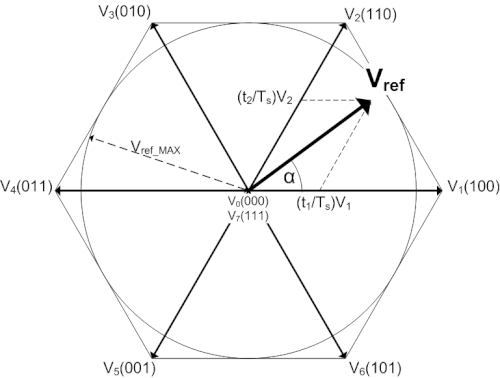
\includegraphics[width=0.5\linewidth]{space-vector-modulation.png}
    \caption{Space Vector Modulation}
    \label{fig:space-vector-modulation}
\end{figure}

The same construction may be applied to each pair of adjacent active vectors. Consequently, the voltage hexagon may be divided into six $60^\circ$ sectors, where an arbitrary reference vector within a given sector may be synthesized from the two active vectors bounding that sector together with either zero vector.

Lastly, notice that connecting the tips of the inverter voltage space vectors forms a hexagon that bounds the space of realizable average vectors. Within this limit, the largest rotating vector of constant magnitude is defined by the hexagon's inscribed circle. This subject is the topic of the following section.


%=========================================================================%
\subsubsection{Acheivable Voltage Vectors}
\label{sec:acheivable-voltage-vectors}
%=========================================================================%

Because the switching durations cannot be negative and their sum cannot exceed the switching period, the achiveable average voltage vectors are bounded by the six active switching vectors. Recall from Section \ref{sec:inverter-switching-states-and-space-vectors} that the six active vectors are separated by $60^\circ$ and have equal magnitudes:

\begin{equation}
    |\mathbf{V}_k| = \frac{2V_{DC}}{3}
\end{equation}

The six vectors therefore form the vertices of a regular haxagon in the $\alpha\beta$ plane. By switching between adjacent active vectors and the zero vectors, any average voltage vector lying within this hexagon may be synthesized.

Thus, while the inverter has only eight possible instantaneous voltage vectors, its acheivable swtiching period average voltage is continuous over the interior of the voltage hexagon:

\begin{equation}
    \overline{\mathbf{V}} \in \mathcal{H}
\end{equation}

Where $\mathcal{H}$ denotes the hexagonal region bounded by the six active voltage vectors. Although the entire interior of the voltage hexagon represetns the achievable average voltage vectors, a balanced sinusoidal three-phase voltage corresponds to a voltage space vector which rotates continuously in the $\alpha\beta$ plane with constant magnitude.

For such a vector to remain achievable throughout an entire electrical revolution, it must remain within the voltage hexagon at every angular position. Consequently, the maximum constant magnitude is not the magnitude of the active vectors at the vertices, but rather the radius of the largest circle which can be inscribed within the hexagon, as shown in Figure \ref{fig:space-vector-modulation} and \ref{fig:max-rotating-space-vector}. 

We can see that the largest inscribed circle has a radius defined by the midsection of the line connecting two of the six active space vectors. Recall that each interior angle of a hexagon measures $120^\circ$. Then, the triangular segment defined by two space vectors and the line connecting their heads must be an equilateral triangle with $60^\circ$ interior angles.

Cutting this triangle in half by drawing a line from the origin to the midpoint between the two space vectors yields two right angle triangles, as shown in Figure \ref{fig:max-rotating-space-vector} by the dashed line. 

\begin{figure}[H]
    \centering
    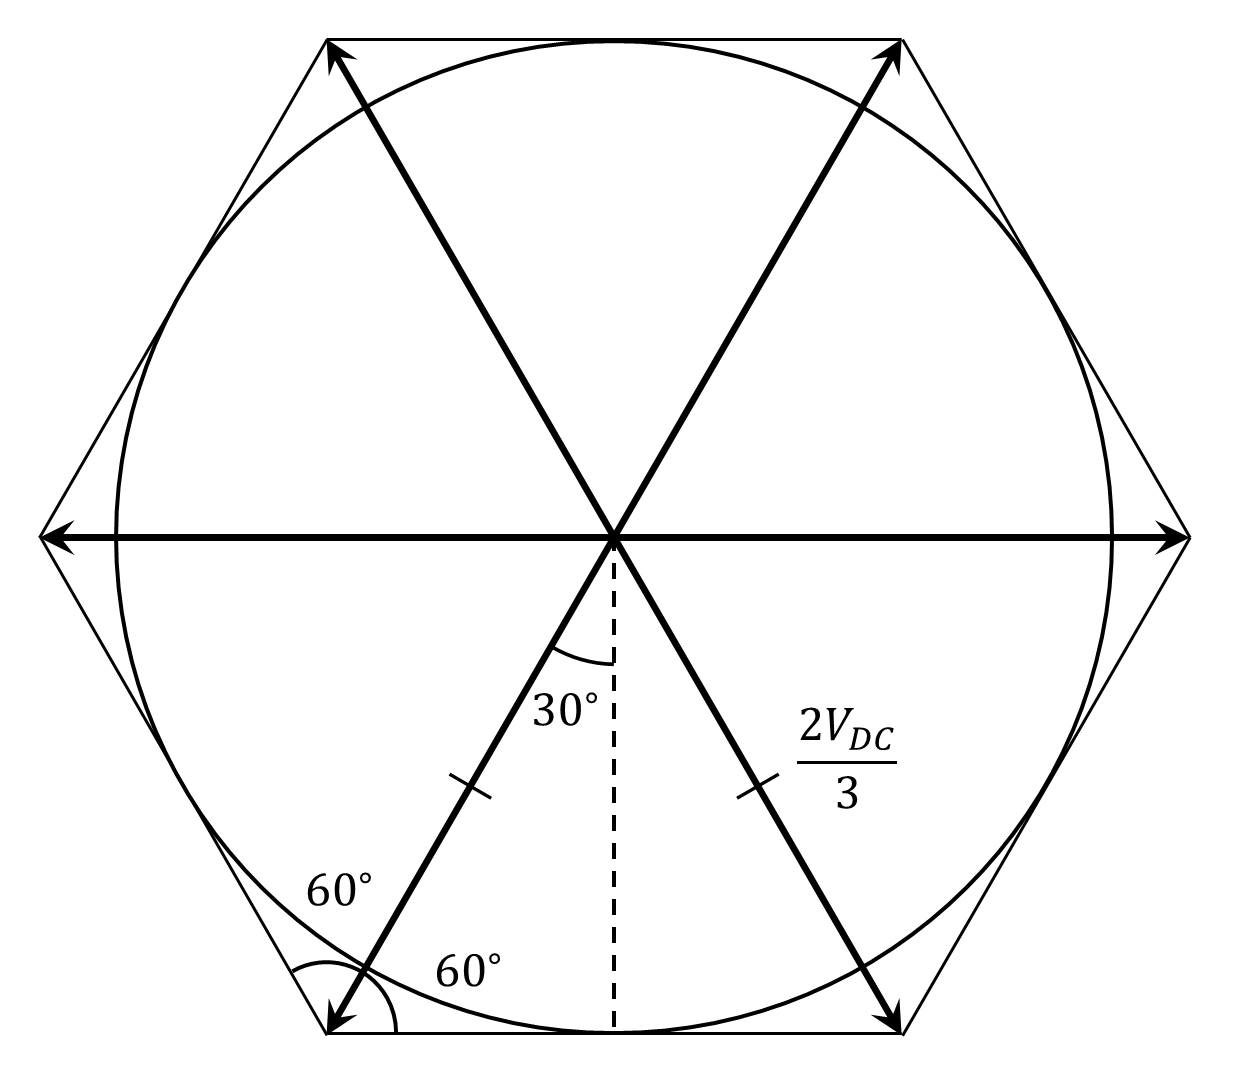
\includegraphics[width=0.45\linewidth]{max-rotating-space-vector.png}
    \caption{Domain of Synthesizable Rotating Vectors of Constant Magnitude}
    \label{fig:max-rotating-space-vector}
\end{figure}

The radius, $r$, of the largest inscribed circle is then the dashed line, which can easily be calculated using trigonometry as:

\begin{equation}
    \sin\theta = \frac{r}{h} \\
\end{equation}

Where $h$ is the hypotneuse, which we know to be the magnitude of the active vector, and $\theta$ is the angle between the hypotneuse and the adjacent component of the triangle. Then, we calculate the radius:

\begin{align}
    r &= h\sin\theta \\
    &= \frac{2V_{DC}}{3}\sin(60^\circ) \\
    &= \frac{2V_{DC}}{3}\frac{\sqrt{3}}{2} \\
    &= \frac{V_{DC}}{\sqrt{3}} 
\end{align}

Thus the maximum magnitude of a constant magnitude rotating average voltage vector which remains entirely within the inverter's linear achiveable voltage region is:

\begin{equation}
    |\mathbf{V}^*|_{max} = \frac{V_{DC}}{\sqrt{3}} = 0.577V_{DC}
\end{equation}

This limit represents the maxmimum available voltage vector magnitude of the ideal inveter when DC link voltage is fully utilized. A particular modulation technique, however, does not necessarily utilize the entire available region. The following sections how different PWM strategies synthesize the desired rotating voltage vector and how effectively they utilize the available DC-link voltage.



%=========================================================================%
\subsection{Sinusoidal Pulse Width Modulation (SPWM)}
\label{sec:spwm}
%=========================================================================%

Sinusoidal pulse-width modulation (SPWM) is a modulation technique used to synthesize approximately sinusoidal three-phase voltages from the discrete switching states of a voltage source inverter. As established in the previous section, the switching-period average voltage of each inverter leg is determined by its duty cycle. Therefore, by continuously varying the duty cycles according to sinusoidal reference signals, the average inverter output voltages can be made to follow sinusoidal waveforms. Notably, SPWM does not require feedback like some other methods, and can be run completely open loop.

For a three-phase inverter, SPWM uses three sinusoidal reference signals displaced from one another by $120^\circ$. Each reference determines the duty cycle of its corresponding inverter leg and, when compared against a common high-frequency carrier waveform, produces the switching signals applied to the inverter switches.

For a sinusoidal PMSM, balanced sinusoidal stator currents produce a rotating stator magnetic field of approximately constant magnitude. When this field is maintained at an appropriate angle relative to the permanent-magnet rotor field, the interaction between the two fields produces smooth electromagnetic torque. Consequently, sinusoidal stator currents are desirable for generating a rotating magnetic field, minimizing torque ripple and efficiently producing the desired fundamental torque.

However, the stator currents cannot be commanded directly by the inverter. Instead, the inverter applies voltages across the motor windings, which cause the currents to evolve according to the electrical dynamics of the machine. Therefore, the immediate objective of the modulation scheme is to synthesize the appropriate stator voltages required to produce the desired stator currents.

The desired phase-to-neutral voltages are defined as:

\begin{equation}
    v_{an}^* = V_m\cos(\theta_e)
\end{equation}

\begin{equation}
    v_{bn}^* = V_m\cos(\theta_e - \frac{2\pi}{3})
\end{equation}

\begin{equation}
    v_{cn}^* = V_m\cos(\theta_e + \frac{2\pi}{3})
\end{equation}

Where:

\begin{equation}
    \theta_e = \omega_e t
\end{equation}

However, not only can the inverter considered in this case not produce negative pole voltages, as discussed in Section \ref{sec:phase-voltages}, it cannot directly apply a phase-to-neutral voltages either. The inverter can only produce voltages with respect to its reference. Therefore, we produce fast averaged sinusoidal inverter pole voltages with a common mode offset of $V_{DC}/2$:

\begin{equation}
    \overline{v}_{ag}^* = \frac{V_{DC}}{2} + v_{an}^* = \frac{V_{DC}}{2} + V_m\cos(\theta_e)
\end{equation}

\begin{equation}
    \overline{v}_{bg}^* = \frac{V_{DC}}{2} + v_{bn}^* =\frac{V_{DC}}{2} + V_m\cos(\theta_e - \frac{2\pi}{3})
\end{equation}

\begin{equation}
    \overline{v}_{cg}^* = \frac{V_{DC}}{2} + v_{cn}^* = \frac{V_{DC}}{2} + V_m\cos(\theta_e + \frac{2\pi}{3})
\end{equation}

Where $V_m \leq V_{DC}/2$ since the inverter cannot produce voltage above $V_{DC}$ or below ground. From Section \ref{sec:phase-voltages}, according to Equation \ref{eqn-v-ng}, the neutral-ground voltage is calculated as:

\begin{equation}
    v_{ng} = \frac{1}{3}(v_{ag} + v_{bg} + v_{cg}) - \frac{1}{3}(v_{an} + v_{bn} + v_{cn})
\end{equation}

Substituting the inverter pole voltages:

\begin{equation}
    v_{ng} = \frac{V_{DC}}{2} + \frac{1}{3}(v_{an}^* + v_{bn}^* + v_{cn}^*) - \frac{1}{3}(v_{an}^* + v_{bn}^* + v_{cn}^*)
\end{equation}

Because phase voltages are balanced:

\begin{equation}
    v_{an}^* + v_{bn}^* + v_{cn}^* = 0
\end{equation}

The neutral-ground voltage is then:

\begin{equation}
    v_{ng} = \frac{V_{DC}}{2}
\end{equation}

Lastly, recall from Section \ref{sec:line-voltages} that a zero-sequence voltage added to each phase (i.e the same voltage constant added to each phase) has no effect on the line voltages:

\begin{equation}
    v_{ab} = v_{an} - v_{bn} = v_{ag} - v_{bg}
\end{equation}

The same voltage can be added to all three pole voltage commands without changing the voltage between motor windings. Note that we aren't fundamentally required to choose $V_{DC}/2$ as the common mode component. Later, we will exploit this freedom to improve upon SPWM. To convert the pole voltage references into duty cycles, recall from Section \ref{sec:fast-averaged-signals} the equations for generating a fast averaged signal using PWM: 

\begin{equation}
    \overline{v}_{ag} = D_aV_{DC}, \qquad
    \overline{v}_{bg} = D_bV_{DC}, \qquad
    \overline{v}_{cg} = D_cV_{DC}
\end{equation}

Recall that $\theta_e = \omega_e t$ and that the duty cycles, $D_a$, $D_b$ and $D_c$ are therefore time-varying. Substituting, we obtain:

\begin{equation}
    D_a = \frac{\overline{v}_{ag}^*}{V_{DC}} = \frac{1}{2} + \frac{V_m}{V_{DC}}\cos(\theta_e)
\end{equation}

\begin{equation}
    D_b = \frac{\overline{v}_{bg}^*}{V_{DC}} = \frac{1}{2} + \frac{V_m}{V_{DC}}\cos(\theta_e - \frac{2\pi}{3})
\end{equation}

\begin{equation}
    D_c = \frac{\overline{v}_{cg}^*}{V_{DC}} = \frac{1}{2} + \frac{V_m}{V_{DC}}\cos(\theta_e + \frac{2\pi}{3})
\end{equation}

Thus, at a certain time $t$ and for a certain electrical frequency $f_e$, for a commanded sinusoidal voltage, a microcontroller can calculate or look up the required cosine values in order to produce the corresponding duty cycles for each inverter phase leg. If we define the modulation index, $M$, as:

\begin{equation}
    M = \frac{2V_m}{V_{DC}}
\end{equation}

Then:

\begin{equation}
\label{eqn:Da-spwm}
    D_a = \frac{1}{2}[1 + M\cos(\theta_e)]
\end{equation}

\begin{equation}
\label{eqn:Db-spwm}
    D_b = \frac{1}{2}[1 + M\cos(\theta_e - \frac{2\pi}{3})]
\end{equation}

\begin{equation}
\label{eqn:Dc-spwm}
    D_c = \frac{1}{2}[1 + M\cos(\theta_e + \frac{2\pi}{3})]
\end{equation}

Any realizable duty cycle must satisfy:

\[
    0 \leq D \leq 1
\]

The maximum duty cycle will occur when $\cos(\theta - \phi) = 1$. Likewise, the minimum duty cycle will occur when $\cos(\theta - \phi) = -1$:

\begin{equation}
    D_{max} = \frac{1}{2}[1 + M] \leq 1
\end{equation}

\begin{equation}
    D_{min} = \frac{1}{2}[1 - M] \geq 0
\end{equation}

Solving both equations for M and summarizing:

\begin{equation}
    V_m = M\frac{V_{DC}}{2}, \qquad
    M \leq 1
\end{equation}

In general, increasing $V_m$ increases the voltage applied to the stator windings, allowing the stator current to increase. An increase in the torque-producing component of current results in greater electromagnetic torque, which causes the motor to accelerate when the developed torque exceeds the opposing load torque. Conversely, reducing the applied voltage can reduce the stator current and developed torque, allowing the motor to decelerate under load. Thus, control of the applied voltage magnitude provides a means of influencing the motor current, torque, and ultimately its rotational speed.


%=========================================================================%
\subsubsection{SPWM Limitations}
%=========================================================================%

SPWM attempts to produce three-phase balanced voltages:

\begin{equation}
    v_{an}^* = V_m\cos(\theta_e)
\end{equation}

\begin{equation}
    v_{bn}^* = V_m\cos(\theta_e - \frac{2\pi}{3})
\end{equation}

\begin{equation}
    v_{cn}^* = V_m\cos(\theta_e + \frac{2\pi}{3})
\end{equation}

Using the reference pole voltages:

\begin{equation}
    \overline{v}_{ag}^* = \frac{V_{DC}}{2} + V_m\cos(\theta_e)
\end{equation}

\begin{equation}
    \overline{v}_{bg}^* = \frac{V_{DC}}{2} + V_m\cos(\theta_e - \frac{2\pi}{3})
\end{equation}

\begin{equation}
    \overline{v}_{cg}^* = \frac{V_{DC}}{2} + V_m\cos(\theta_e + \frac{2\pi}{3})
\end{equation}

The resulting $\alpha\beta$ frame voltage vector is therefore, per Section \ref{sec-amp-invar-clarke}:

\begin{equation}
    |\mathbf{V}_s| =
    \begin{bmatrix}
        v_\alpha \\
        v_\beta
    \end{bmatrix}
    = V_m
    \begin{bmatrix}
        cos(\theta_e) \\
        sin(\theta_e)
    \end{bmatrix}
\end{equation}

Therefore, $|\mathbf{v}_s| = V_m$. Earlier, we defined $V_m$ as:

\begin{equation}
    V_m = M\frac{V_{DC}}{2}
\end{equation}

$V_m$ cannot be defined any larger since $|v_{xg}| \leq V_{DC}$. The maximum sinusoidal phase-voltage amplitude in linear SPWM is therefore:

\begin{equation}
    V_{m,max} = \frac{V_{DC}}{2}, \qquad M = 1
\end{equation}

In otherwords, conventional SPWM can only produce a rotating reference vector with a maximum magnitude of:

\begin{equation}
    |\mathbf{V}_s^*|_{max}^{SPWM} = \frac{V_{DC}}{2}
\end{equation}

However, recall from Section \ref{sec:acheivable-voltage-vectors} that the maximum achiveable magnitude for a rotating voltage vector synthesized by a two-level three-phase inverter is:

\begin{equation}
    |\mathbf{V}_s^*|_{max}^{inverter} = \frac{V_{DC}}{\sqrt{3}}
\end{equation}

And therefore:

\begin{equation}
    \frac{V_{DC}/2}{V_{DC}/\sqrt{3}} = \frac{\sqrt{3}}{2} \approx 0.866
\end{equation}

So, conventional SPWM uses only 86.6\% of the maxmimum linear voltage vector magnitude available from the inverter. 


%=========================================================================%
\subsubsection{Practical Implemention of SPWM}
%=========================================================================%

For a machine with $p$ pole pairs ($2p$ poles in total), for a desired speed in RPM:

\begin{equation}
    \omega_m = \frac{2\pi \times RPM}{60}
\end{equation}

This yields an electrical angular velocity and a commanded stator electrical frequency respectively of:

\begin{equation}
    \omega_s = p\omega_m
\end{equation}

\begin{equation}
    f_s = \frac{\omega_s}{2\pi}
\end{equation}

At the beginning of every PWM period, or every $50\mu s$ ($T_s = 1/20,000 = 50\mu s$), the electrical angle is first advanced:

\begin{equation}
    \Delta\theta_s = \omega_sT_s
\end{equation}

Note that in open-loop SPWM, the electrical angle used to generate the three-phase voltage references represents the commanded stator voltage angle, not the actual rotor electrical angle. The rotor develops its own angular displacement relative to this rotating excitation, and it is this difference which is responsible for torque production. If we recall Section \ref{sec-park-transformation}, transforming a sinusoidal three-phase quantity to $dq$ frame yields a DC quantity entirely along the $d$ axis. We also know from Section \ref{sec:electromagnetic-torque} that $q$-axis current is entirely responsible for torque production in a non-salient machine. Hence this inaccuracy between the actual and commanded electrical angle is both a pitfall of the system and the reason it functions in the first place.

Moving on, the modulation index, $M$ must be chosen sufficently large for the motor to maintain synchronism with the commanded electrical frequency. If the applied voltage is insufficent, the motor may be unable to produce the torque required to follow the rotating stator field. If $M$ is chosen too high, an unnecessarily high current may be driven into the motor, causing increased losses, heating and possibly damage.

In a simple open loop implementation, the modulation index may be varied approximately in proportion to the commanded electrical frequency, commonly referred to as volts-per-hertz ($V/f$) control. As motor speed increases, the increasing back-EMF requires a correspondingly larger applied stator voltage. At steady state and light/no load:

\[
    i_d \approx i_q \approx 0
\]

And:

\[
    \frac{di_d}{dt} \approx \frac{di_q}{dt} \approx 0
\]

From the PMSM model: 

\begin{equation}
    v_d = R_si_d + L_d\frac{di_d}{dt} - \omega_eL_qi_q \approx 0
\end{equation}

\begin{equation}
    v_q = R_si_q + L_q\frac{di_q}{dt} + \omega_eL_di_d + \omega_e\lambda_m \approx \omega_e\lambda_m
\end{equation}

Since the magnitude of the $\alpha\beta$ vector is preserved in $dq$ frame and vice versa, substituting $\omega_s$, the required stator voltage vector magnitude is:

\begin{equation}
    V_m = \sqrt{v_d^2 + v_q^2} \approx \omega_s\lambda_m
\end{equation}

Recall that:

\begin{equation}
    V_m = M\frac{V_{DC}}{2}
\end{equation}

Substituting and rearranging:

\begin{equation}
    M \approx \frac{2\omega_s\lambda_m}{V_{DC}}, \qquad
    0 \leq M \leq 1
\end{equation}

Then, using the electrical angle increment and the modulation index, we calculate the duty cycles.

\begin{equation}
    D_a = \frac{1}{2}[1 + M\cos(\theta_s + \Delta\theta_s)]
\end{equation}

\begin{equation}
    D_b = \frac{1}{2}[1 + M\cos(\theta_s + \Delta\theta_s - \frac{2\pi}{3})]
\end{equation}

\begin{equation}
    D_c = \frac{1}{2}[1 + M\cos(\theta_s + \Delta\theta_s + \frac{2\pi}{3})]
\end{equation}

These duty cycles are typically commanded to a timer peripheral within a microcontroller, which converts the duty cycles into the corresponding PWM cycle. This process then repeats, once per PWM period. 

This represents a relatively simple open-loop implementation of SPWM. Since no feedback is used, the controller has no direct knowledge of the actual rotor speed, position, or loading, and therefore cannot actively compensate for disturbances such as changes in mechanical load or variations in motor parameters. Consequently, the commanded electrical frequency and modulation index may not remain appropriate as operating conditions change. These limitations can be addressed through closed-loop control using measurements of the motor state. Since the primary focus of this document is field-oriented control (FOC), more advanced open-loop SPWM control techniques will not be considered further.


%=========================================================================%
\subsection{Third Harmonic Injection}
\label{sec:third-harmonic-injection}
%=========================================================================%

In Section \ref{sec:spwm}, conventional sinusoidal pulse-width modulation was shown to produce a maximum rotating voltage vector magntiude of:

\begin{equation}
    |\mathbf{V}_s^*|_{max}^{SPWM} = \frac{V_{DC}}{2}
\end{equation}

However, Section \ref{sec:switching-vectors-and-time-averaging} established that the maximum constant magnitude rotating voltage vector which can remain entirely within the achievable voltage hexagon is:

\begin{equation}
    |\mathbf{V}_s^*|_{max}^{inverter} = \frac{V_{DC}}{\sqrt{3}}
\end{equation}

Therefore, conventional SPWM does not fully utilize the available DC-link voltage. The reason for this limitation is not the fundamental voltage capability of the inverter, but rather the particular common-mode voltage used to construct the three inverter pole voltage references.

Recall from Section \ref{sec:spwm} that the conventional SPWM pole voltage references were constructed as:

\begin{equation}
    \overline{v}_{ag}^* = \frac{V_{DC}}{2} + V_m\cos(\theta_e)
\end{equation}

\begin{equation}
    \overline{v}_{bg}^* = \frac{V_{DC}}{2} + V_m\cos(\theta_e - \frac{2\pi}{3})
\end{equation}

\begin{equation}
    \overline{v}_{cg}^* = \frac{V_{DC}}{2} + V_m\cos(\theta_e + \frac{2\pi}{3})
\end{equation}

The common offset $V_{DC}/2$ centers the three sinusoidal references within the available inverter pole voltage range. In other words, the floating point neutral is shifted to a potential of $V_{DC}/2$ with respect to ground. Then, since $v_{xn} = v_{xg} - v_{ng}$:

\begin{equation}
    v_{an}^* = V_m\cos(\theta_e)
\end{equation}

\begin{equation}
    v_{bn}^* = V_m\cos(\theta_e - \frac{2\pi}{3})
\end{equation}

\begin{equation}
    v_{cn}^* = V_m\cos(\theta_e + \frac{2\pi}{3})
\end{equation}

However, $V_{DC}/2$ is not the only common mode voltage that may be added to the three pole voltage references. The aim of Third Harmonic Injection (THI) is to provide a continuously varying neutral point voltage through zero sequence voltage injection such that the motor is better able to make use of the available DC bus voltage. As with SPWM, this injected zero sequence voltage does not affect the phase or line voltages, however does affect the pole and neutral voltages. The result is balanced three phase, phase voltages with a greater allowable magnitude compared to SPWM.


%=========================================================================%
\subsubsection{Common-Mode Voltage Injection}
\label{sec:common-mode-voltage-injection}
%=========================================================================%

In this section, we show that we can add any arbitrary voltage component equally to each inverter pole voltage without alterning the phase or line voltages. In the next section, we will see why this is useful. From Section \ref{sec:phase-voltages}, at every instant in time:

\begin{equation}
    v_{an} = v_{ag} - v_{ng}, \qquad
    v_{bn} = v_{bg} - v_{ng}, \qquad
    v_{cn} = v_{cg} - v_{ng}
\end{equation}

Taking the average over one PWM period:

\begin{equation}
    \overline{v}_{an} = \overline{v}_{ag} - \overline{v}_{ng}, \qquad
    \overline{v}_{bn} = \overline{v}_{bg} - \overline{v}_{ng}, \qquad
    \overline{v}_{cn} = \overline{v}_{cg} - \overline{v}_{ng}
\end{equation}

Ideally, pulse-width modulation attempts to generate a modulated signal which averages to approximate the reference signal. At the inverter poles:

\begin{equation}
    \overline{v}_{ag} \approx v_{ag}^*, \qquad
    \overline{v}_{bg} \approx v_{bg}^*, \qquad
    \overline{v}_{cg} \approx v_{cg}^*
\end{equation}

The pole voltage produces some phase voltage referenced to the isolated neutral. The control objective is therefore:

\begin{equation}
    \overline{v}_{an} \approx v_{an}^*, \qquad
    \overline{v}_{bn} \approx v_{bn}^*, \qquad
    \overline{v}_{cn} \approx v_{cn}^*
\end{equation}

From Section \ref{sec:phase-voltages}, recall the floating neutral voltage equation:

\begin{equation}
    v_{ng} = \frac{1}{3}(v_{ag} + v_{bg} + v_{cg}) - \frac{1}{3}(v_{an} + v_{bn} + v_{cn}) 
\end{equation}

For the balanced machine considered:

\begin{equation}
    v_{an} + v_{bn} + v_{cn} = 0
\end{equation}

Therefore, instantaneously:

\begin{equation}
    v_{ng} = \frac{1}{3}(v_{ag} + v_{bg} + v_{cg})
\end{equation}

Averaging across one PWM period gives:

\begin{equation}
    \overline{v}_{ng} = \frac{1}{3}(\overline{v}_{ag} + \overline{v}_{bg} + \overline{v}_{cg})
\end{equation}

We define this quantity as the common-mode voltage. It is calculated as the average of all three inverter pole voltages, and we denote this as:

\begin{equation}
    v_{cm} \equiv \frac{1}{3}(v_{ag} + v_{bg} + v_{cg})
\end{equation}

So:

\begin{equation}
    v_{ng} = v_{cm}
\end{equation}

Consider the desired phase voltages:

\begin{equation}
    v_{an}^* = V_m\cos(\theta_e)
\end{equation}

\begin{equation}
    v_{bn}^* = V_m\cos(\theta_e - \frac{2\pi}{3})
\end{equation}

\begin{equation}
    v_{cn}^* = V_m\cos(\theta_e + \frac{2\pi}{3})
\end{equation}

Where the $"*"$ denotes desired/reference. Since they are balanced:

\begin{equation}
\label{eqn:balanced-desired}
    v_{an}^* + v_{bn}^* + v_{cn}^* = 0
\end{equation}

However, recall that we cannot produce phase voltages directly. The inverter bridge can only produce pole voltages, $v_{ag}$, $v_{bg}$ and $v_{cg}$. Hence we construct pole-voltage commands including an additional commmon-mode component:

\begin{equation}
    v_{ag}^* = v_{an}^* + v_{cm}^*, \qquad
    v_{bg}^* = v_{bn}^* + v_{cm}^*, \qquad
    v_{cg}^* = v_{cn}^* + v_{cm}^*
\end{equation}

Where since $v_{cm}$ is defined as the average pole voltage, we have the ability to establish any common-mode voltage desirable, $v_{cm}^*$, provided we stay within the DC bus limits. SPWM is simply one possible choice for this common-mode voltage. Recall from Section \ref{sec:spwm} that we defined the common-mode voltage (then denoted as the neutral-ground voltage $v_{ng}$) as:

\begin{equation}
    v_{cm}^* = \frac{V_{DC}}{2}
\end{equation}

So:

\begin{equation}
    v_{ag}^* = v_{an}^* + \frac{V_{DC}}{2}
\end{equation}

$V_{DC}/2$ was selected because the commanded phase voltage $v_{an}^*$ swings postive and negative about zero, while the inverter pole command must lie between:

\[
    0 \leq v_{ag}^* \leq V_{DC}
\]

Hence the entire waveform was lifted by $V_{DC}/2$. As a result, the constraint on the amplitude of the commanded sine was introduced to remain within these the DC bus limits. However, as we eluded to earlier, we have the ability to selected any common-mode voltage within the DC bus limits, including voltages which are time-varying. If we instead select a time varying common-mode voltage such as:

\begin{equation}
    v_{cm}^*(t) = \frac{V_{DC}}{2} + v_{inj}(t)
\end{equation}

And therefore command:

\begin{equation}
    v_{ag}^* = v_{an}^* + \frac{V_{DC}}{2} + v_{inj}
\end{equation}

\begin{equation}
    v_{bg}^* = v_{bn}^* + \frac{V_{DC}}{2} + v_{inj}
\end{equation}

\begin{equation}
    v_{cg}^* = v_{cn}^* + \frac{V_{DC}}{2} + v_{inj}
\end{equation}

Using PWM, we modulate the commanded inverter pole voltages:

\begin{equation}
    \overline{v}_{ag} \approx v_{ag}^*, \qquad
    \overline{v}_{bg} \approx v_{bg}^*, \qquad
    \overline{v}_{cg} \approx v_{cg}^*
\end{equation}

The resultant neutral voltage becomes:

\begin{align}
    \overline{v}_{ng}
    &= \frac{1}{3}(\overline{v}_{ag} + \overline{v}_{bg} + \overline{v}_{cg}) \\
    &\approx \frac{1}{3}(v_{ag}^* + v_{bg}^* + v_{cg}^*) \\
    &\approx \frac{1}{3}(v_{an}^* + v_{bn}^* + v_{cn}^* + 3v_{cm}^*)
\end{align}

However, the sum of balanced phase voltage is zero, therefore:

\begin{equation}
    \overline{v}_{ng} \approx v_{cm}^*
\end{equation}

Or:

\begin{equation}
    \overline{v}_{ng} = \frac{V_{DC}}{2} + v_{inj}
\end{equation}

Then, the phase voltages the motor is provided:

\begin{equation}
    \overline{v}_{an} = \overline{v}_{ag} - \overline{v}_{ng}, \qquad
    \overline{v}_{bn} = \overline{v}_{bg} - \overline{v}_{ng}, \qquad
    \overline{v}_{cn} = \overline{v}_{cg} - \overline{v}_{ng}
\end{equation}

Under ideal PWM, the inverter pole voltages approximately follow the references:

\begin{equation}
    \overline{v}_{ag} \approx v_{ag}^*, \qquad
    \overline{v}_{bg} \approx v_{bg}^*, \qquad
    \overline{v}_{cg} \approx v_{cg}^*
\end{equation}

And:

\begin{equation}
    \overline{v}_{ng} \approx v_{cm}^*
\end{equation}

Therefore:

\begin{equation}
    \overline{v}_{an} \approx v_{ag}^* + v_{cm}^*, \qquad
    \overline{v}_{bn} \approx v_{bg}^* + v_{cm}^*, \qquad
    \overline{v}_{cn} \approx v_{cg}^* + v_{cm}^*
\end{equation}

However, we know that:

\begin{equation}
    v_{ag}^* = v_{an}^* + v_{cm}^*, \qquad
    v_{bg}^* = v_{bn}^* + v_{cm}^*, \qquad
    v_{cg}^* = v_{cn}^* + v_{cm}^*
\end{equation}

Therefore:

\begin{equation}
    \overline{v}_{an} \approx v_{an}^* + v_{cm}^* - v_{cm}^*, \qquad
    \overline{v}_{bn} \approx v_{bn}^* + v_{cm}^* - v_{cm}^*, \qquad
    \overline{v}_{cn} \approx v_{cn}^* + v_{cm}^* - v_{cm}^*
\end{equation}

And finally:

\begin{equation}
    \overline{v}_{an} \approx v_{an}^*, \qquad
    \overline{v}_{bn} \approx v_{bn}^*, \qquad
    \overline{v}_{cn} \approx v_{cn}^*
\end{equation}

In summary, by adding the same common-mode voltage to all three pole-voltage references, the inverter can shift the floating neutral voltage without altering the desired phase-to-neutral voltages seen by the motor. Similarly, this is also true of the line-to-line voltages, as shown in Section \ref{sec:line-voltages} in a much more straight forward derivation. This freedom allows the pole voltage references to be repositioned within the avilable DC bus range, forming the basis for improved DC-bus utilization through third harmonic injection.


%=========================================================================%
\subsubsection{Third Harmonic Voltage Injection}
\label{sec:third-harmonic-voltage-injection}
%=========================================================================%

In Section \ref{sec:acheivable-voltage-vectors}, we found that the maximum magnitude of a constant rotating voltage vector that can be synthesized by a two-level, three-phase inverter is $0.577V_{DC}$. However, SPWM is limited to $0.5V_{DC}$, utilizing only $86.6\%$ of this available linear voltage capability. Third-harmonic injection (THI) overcomes this limitation by adding a third-harmonic common-mode voltage to the three phase references, allowing the fundamental amplitude to be increased by $15.47\%$ without altering the line-to-line voltages.

While the choice of a third harmonic may initally seem arbitrary, suppose for now that it is injected as a common-mode component and examine the resulting effect. The injected third harmonic is written as:

\begin{equation}
    v_{inj}(\theta_e) = V_3\cos(3\theta_e)
\end{equation}

Such that the three commanded pole voltages become:

\begin{equation}
    v_{ag}^* = V_m\cos(\theta_e) + \frac{V_{DC}}{2} + V_3\cos(3\theta_e)
\end{equation}

\begin{equation}
    v_{bg}^* = V_m\cos(\theta_e - \frac{2\pi}{3}) + \frac{V_{DC}}{2} + V_3\cos(3\theta_e)
\end{equation}

\begin{equation}
    v_{cg}^* = V_m\cos(\theta_e + \frac{2\pi}{3}) + \frac{V_{DC}}{2} + V_3\cos(3\theta_e)
\end{equation}

Where the desired common-mode voltage is:

\begin{equation}
    v_{cm}^* = \frac{V_{DC}}{2} + V_3\cos(3\theta_e)
\end{equation}

Notice that rearranging the third harmonic for phases-$b$ and -$c$:

\begin{equation}
    \cos(3(\theta_e - \frac{2\pi}{3})) = \cos(3\theta_e - 2\pi) = \cos(3\theta_e)
\end{equation}

\begin{equation}
    \cos(3(\theta_e + \frac{2\pi}{3})) = \cos(3\theta_e + 2\pi) = \cos(3\theta_e)
\end{equation}

Thus, the $120^\circ$ displacement between the fundamental phase quantities corresponds to a $360^\circ$ displacement at the third harmonic. Since a $360^\circ$ displacement is equivalent to no phase displacement at all, the third harmonic is in phase with all three phases. This can be seen in Figure \ref{fig:third-harmonic}, where the third harmonic contributes the same amount to each phase as corresponding points in the fundamental electrical cycle.

\begin{figure}[H]
    \centering
    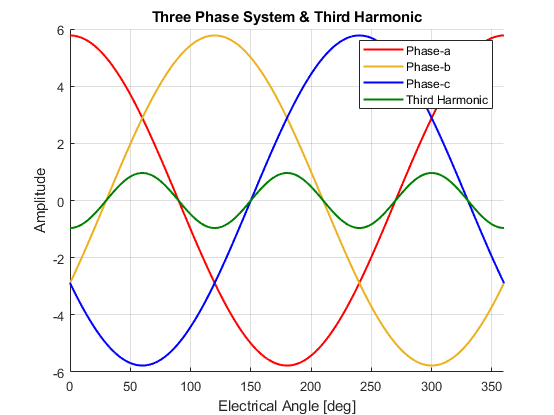
\includegraphics[width=0.51\linewidth]{third-harmonic.png}
    \caption{Balanced Three Phase System with Third Harmonic}
    \label{fig:third-harmonic}
\end{figure}

This reveals one reason why the third harmonic is a convenient choice for common-mode injection. Although an arbitrary waveform could instead be added equally to all three pole-voltage references, the third harmonic naturally possesses the $120^\circ$ periodicity of the three-phase system. Furthermore, since it is injected as a common-mode component, it does not affect the resulting phase-to-phase voltages.

Now we can begin to understand this selection. By injecting an inverted third harmonic to each pole voltage, we reduce the peaks of the pole voltage references. Simultaneously, since the neutral voltage is equivalent to the common-mode voltage for a balanced system, the neutral voltage also shifts according to the injected third harmonic. This is much more easily seen visually in Figure \ref{fig:third-harmonic-injection-waveforms}.

\begin{figure}[H]
    \centering
    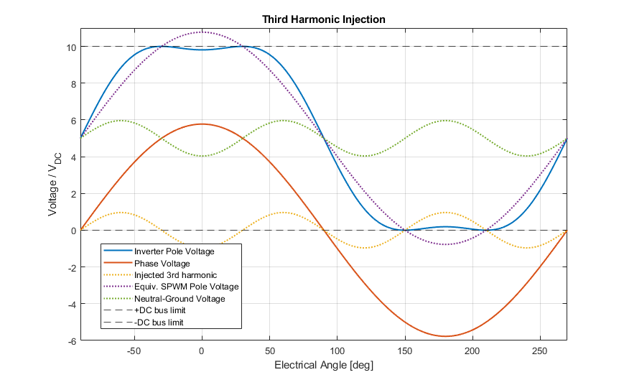
\includegraphics[width=0.8\linewidth]{third-harmonic-injection-waveforms.png}
    \caption{Third Harmonic Injection Waveforms for One Phase}
    \label{fig:third-harmonic-injection-waveforms}
\end{figure}

From Figure \ref{fig:third-harmonic-injection-waveforms}, we can see that by adding the inverted third harmonic (yellow) to the traditional SPWM pole voltage reference (purple) results in the THI pole voltage shown in blue. By adding a common-mode component equal to the third harmonic plus half the DC bus voltage, we shift the floating neutral point to the curve shown in green. Then, since the phase voltage is the difference between the inverter pole voltage and the neutral voltage, where both components contain the DC offset and third harmonic, the common-mode terms present in both quantities cancel, leaving a purely sinusoidal phase voltage.

Most importantly, the fundamental components of the THI and SPWM pole voltage references both have the same amplitude of $V_{DC}/2$. However, while the SPWM reference reaches the upper and lower DC-bus limits, the injected thrid harmonic pulls the peaks of the THI reference away from these limits. Thus, THI creates additional voltage headroom while maintaining the same fundamental phase voltage. This headroom can subsequently be used to increase the commanded fundamental voltage amplitude.

To accomplish this, the amplitude of the injected third harmonic must be selected such that the peak magnitude of the inverter pole-voltage reference is minimized for a given fundamental voltage amplitude. Minimization of the resulting reference waveform, is a long and tedious derivation which provides very little insight or intuition for understanding THI. The derivation is therefore deferred to Appendix \ref{app:thi-optimiazation} The final result however, is provided as:

\begin{equation}
    V_3 = -\frac{V_m}{6}
\end{equation}

Thus, if we define the AC component of the phase-$a$ pole-voltage as:

\begin{equation}
    f(\theta_e) = V_m\cos\theta_e + V_3\cos3\theta_e
\end{equation}

This becomes:

\begin{equation}
    f(\theta_e) = V_m(\cos\theta_e - \frac{1}{6}\cos3\theta_e)
\end{equation}

Although the fundamental component has an amplutde $V_m$, the addition of the third harmonic reduces the maximum magnitude of the combined reference waveform. Per Appendix \ref{app:thi-optimiazation}, the extrema of this waveform occur at $\theta_e = \pi/6$ and its periodic equivalents, where:

\begin{equation}
    |f(\theta_e)|_{max} = \frac{\sqrt{3}}{2}V_m, \qquad
    \theta_e = \frac{\pi}{6}
\end{equation}

Since the pole voltage reference is centered about $V_{DC}/2$, its AC component must reamin within $\pm V_{DC}/2$. Therefore:

\begin{equation}
    \frac{\sqrt{3}}{2}V_m \leq \frac{V_{DC}}{2}
\end{equation}

Giving the maximum achievable fundamental phase voltage amplitude:

\begin{equation}
    \boxed{
        V_{m,max}^{THI} = \frac{V_{DC}}{\sqrt{3}}
        }
\end{equation}

Compared to SPWM:

\begin{equation}
    V_{m,max}^{SPWM} = \frac{V_{DC}}{2}
\end{equation}

Therefore:

\begin{equation}
    \frac{V_{m,max}^{THI}}{V_{m,max}^{SPWM}} = \frac{V_{DC}/\sqrt{3}}{V_{DC}/2} = \frac{2}{\sqrt{3}} \approx 1.1547
\end{equation}

Third-harmonic injection therefore permits a 15.47\% increase in the maximum fundamental phase-voltage amplitude compared with conventional SPWM for the same DC-bus voltage. Importantly, this increase is achieved without introducing third-harmonic content into the motor phase-to-phase voltages, since the injected component is common to all three inverter legs and cancels when the pole-voltage differences are taken.

All three reference signals with respect to ground are illustrated in the Figure \ref{fig:thi-3p-references}.

\begin{figure}[H]
    \centering
    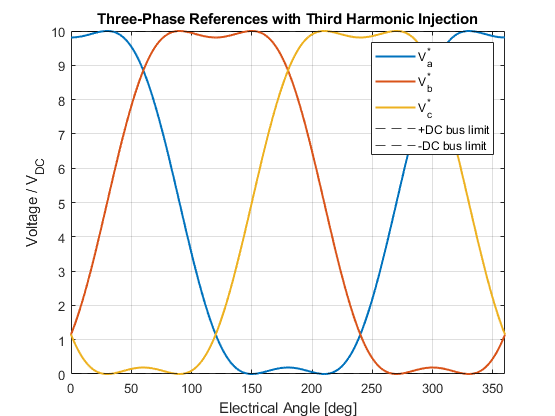
\includegraphics[width=0.6\linewidth]{thi-3p-references.png}
    \caption{Third Harmonic Injection Reference Waveforms}
    \label{fig:thi-3p-references}
\end{figure}

In summary, the equation for each reference signal is:

\begin{equation}
    v_{ag}^* = V_m\left[\cos(\theta_e)  - \frac{1}{6}\cos(3\theta_e)\right] + \frac{V_{DC}}{2}
\end{equation}

\begin{equation}
    v_{bg}^* = V_m\left[\cos(\theta_e - \frac{2\pi}{3}) - \frac{1}{6}\cos(3\theta_e)\right] + \frac{V_{DC}}{2}
\end{equation}

\begin{equation}
    v_{cg}^* = V_m\left[\cos(\theta_e + \frac{2\pi}{3}) - \frac{1}{6}\cos(3\theta_e)\right] + \frac{V_{DC}}{2}
\end{equation}

With:

\begin{equation}
    V_m \leq \frac{V_{DC}}{\sqrt{3}}
\end{equation}

Which yields the phase voltages:

\begin{equation}
    v_{an}^* = V_m\cos(\theta_e)
\end{equation}

\begin{equation}
    v_{bn}^* = V_m\cos(\theta_e - \frac{2\pi}{3})
\end{equation}

\begin{equation}
    v_{cn}^* = V_m\cos(\theta_e + \frac{2\pi}{3})
\end{equation}

Where:

\begin{equation}
    v_{cm}^* = \overline{v}_{ng} = \frac{V_{DC}}{2} - \frac{V_m}{6}\cos3\theta
\end{equation}

To get the duty cycles we apply to each inverter leg, recall from Section \ref{sec:pulse-width-modulation} the relationship between duty cycle, the DC-link voltage, and the average output voltage:

\begin{equation}
    \overline{v}_{ag} = D_aV_{DC}, \qquad
    \overline{v}_{bg} = D_bV_{DC}, \qquad
    \overline{v}_{cg} = D_cV_{DC}
\end{equation}

Rearranging and substituting the desired voltage references:

\begin{equation}
    D_a = \frac{v_{ag}^*}{V_{DC}}, \qquad
    D_b = \frac{v_{bg}^*}{V_{DC}}, \qquad
    D_c = \frac{v_{cg}^*}{V_{DC}}
\end{equation}

Substituting the desired voltage equations:

\begin{equation}
    D_a = \frac{1}{2} + \frac{V_m}{V_{DC}}\left[\cos(\theta_e) - \frac{1}{6}\cos(\theta_e)\right]
\end{equation}

\begin{equation}
    D_b = \frac{1}{2} + \frac{V_m}{V_{DC}}\left[\cos(\theta_e - \frac{2\pi}{3}) - \frac{1}{6}\cos(\theta_e)\right]
\end{equation}

\begin{equation}
    D_c = \frac{1}{2} + \frac{V_m}{V_{DC}}\left[\cos(\theta_e + \frac{2\pi}{3}) - \frac{1}{6}\cos(\theta_e)\right]
\end{equation}

Similar to Section \ref{sec:spwm}, if we define $M$ as:

\begin{equation}
    M = \frac{2V_m}{V_{DC}}
\end{equation}

Then:

\begin{equation}
    D_a = \frac{1}{2}\left[1 + M\left(\cos(\theta_e) - \frac{1}{6}\cos(\theta_e)\right)\right]
\end{equation}

\begin{equation}
    D_b = \frac{1}{2}\left[1 + M\left(\cos(\theta_e - \frac{2\pi}{3}) - \frac{1}{6}\cos(\theta_e)\right)\right]
\end{equation}

\begin{equation}
    D_c = \frac{1}{2}\left[1 + M\left(\cos(\theta_e + \frac{2\pi}{3}) - \frac{1}{6}\cos(\theta_e)\right)\right]
\end{equation}

Where now, due to the third harmonic and since $D \leq 1$:

\begin{equation}
    0 \leq M \leq \frac{2}{\sqrt{3}} \approx 1.1547
\end{equation}

Recall that for SPWM:

\begin{equation}
    0 \leq M_{SPWM} \leq 1
\end{equation}

The modulation index should be selected sufficiently high such that the stator magnetic field can maintain synchronism with the rotor, while avoiding an unnecessarily large applied voltage. Unlike SPWM, however, the addition of the third-harmonic component allows a larger modulation index to be used before entering overmodulation. Therefore, the modulation index may be selected in the same manner as for SPWM, while taking advantage of the increased linear modulation range provided by THI.


%=========================================================================%
\subsubsection{Practical Implemention of Third Harmonic Injection}
%=========================================================================%

One simple open-loop implementation of third harmonic injection is very similar to that of SPWM in Section \ref{sec:spwm}. Given a desired mechanical speed, the desired electrical angular velocity can be calculated. Then, using the PWM period, the angle increment can be updated and added to the current angle counter. 

Then, the modulation index is selected based on the desired stator voltage magnitude. The primary difference between THI and SPWM is that a third harmonic component is added equally to each of the three sinusoidal reference signals. Using the modulation index defined previously for SPWM:

\begin{equation}
    M \approx \frac{2\omega_s\lambda_m}{V_{DC}}, \qquad
    0 \leq M \leq \frac{2}{\sqrt{3}}
\end{equation}

Then, using commanded angle increment and the modulation index, we can calculate the duty cycles:

\begin{equation}
    D_a = \frac{1}{2}\left[1 + M\left(\cos(\theta_s + \Delta\theta_s) - \frac{1}{6}\cos(\theta_s + \Delta\theta_s)\right)\right]
\end{equation}

\begin{equation}
    D_b = \frac{1}{2}\left[1 + M\left(\cos(\theta_s + \Delta\theta_s - \frac{2\pi}{3}) - \frac{1}{6}\cos(\theta_s + \Delta\theta_s)\right)\right]
\end{equation}

\begin{equation}
    D_c = \frac{1}{2}\left[1 + M\left(\cos(\theta_s + \Delta\theta_s + \frac{2\pi}{3}) - \frac{1}{6}\cos(\theta_s + \Delta\theta_s)\right)\right]
\end{equation}

Therefore, only a single third harmonic term must be calculated during each PWM update. The calculated duty cycles can  then be written directly to the corresponding timer compare registers of the microcontroller, in the same manner as conventional PWM.


%=========================================================================%
\subsection{Space Vector Pulse-Width Modulation (SVPWM)}
\label{sec:svpwm}
%=========================================================================%

In Section \ref{sec:inverter-switching-states-and-space-vectors}, it was shown that a two-level, three-phase inverter possesses six active voltage vectors and two zero voltage vectors. In Section \ref{sec:switching-vectors-and-time-averaging}, we found that although the inverter can only occupy one of these eight discrete switching states at any instant, switching between the states within a PWM period allows an arbitrary average voltage vector within the inverter voltage hexagon to be synthesized. Furthermore, Section \ref{sec:acheivable-voltage-vectors} showed that the maximum magnitude of a continuously rotating voltage vector within the linear modulation region is:

\begin{equation}
    |\mathbf{V}_s^*|_{max} = \frac{V_{DC}}{\sqrt{3}}
\end{equation}

Space vector pulse-width modulation (SVPWM), often referred to as space vector modulation (SVM), is a modulation strategy which directly makes use of this voltage vector representation. During each PWM period, the desired stator voltage vector is synthesized by applying the two active voltage vectors surrounding the reference vector for calculated durations, with the remaining portion of the switching period assigned to the zero vectors. 

Unlike SPWM, which synthesizes a rotating magnetic field by modulating voltages based on three sinusoidal references given a commanded stator field angle, SVPWM synthesizes a commanded voltage vector directly given its magnitude and phase.


%=========================================================================%
\subsubsection{Sector-Based SVPWM}
\label{sec:sector-based-svpwm}
%=========================================================================%

Recall that the six active voltage vectors are equally spaced by $60^\circ$ in the stationary $\alpha\beta$ plane. These vectors divide the inverter voltage hexagon into six sectors, as illustrated in Figure \ref{fig:space-vector-modulation2}.

\begin{figure}[H]
    \centering
    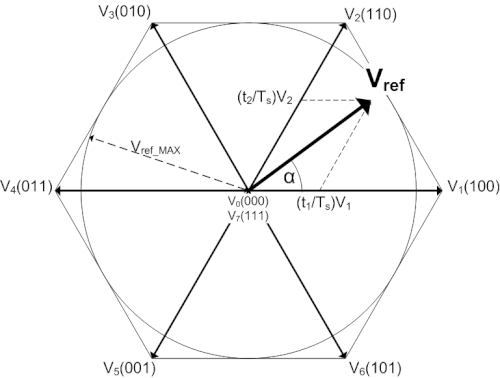
\includegraphics[width=0.4\linewidth]{space-vector-modulation.png}
    \caption{Space Vector Modulation}
    \label{fig:space-vector-modulation2}
\end{figure}

Repeating the Table \ref{tab:inverter_space_vectors} from Section \ref{sec:inverter-switching-states-and-space-vectors} detailing the eight inverter vectors in $\alpha\beta$ frame from their switch configuration/code, $\alpha\beta$ components, magnitude and electrical spatial angle:

\begin{table}[H]
    \centering
    \caption{Inverter Voltage Space Vectors in the $\alpha\beta$ Frame}
    \label{tab:inverter_space_vectors2}

    \renewcommand{\arraystretch}{2.3}
    \setlength{\tabcolsep}{12pt}

    \begin{tabular}{c c c c c c}
        \hline
        \textbf{Vector} &
        $\boldsymbol{S_aS_bS_c}$ &
        $\boldsymbol{v_\alpha}$ &
        $\boldsymbol{v_\beta}$ &
        $\boldsymbol{|\mathbf{V}_k|}$ &
        $\boldsymbol{\theta_k}$ \\
        \hline

        $\mathbf{V}_0$ & $000$
        & $0$
        & $0$
        & $0$
        & -- \\

        $\mathbf{V}_1$ & $100$
        & $\dfrac{2V_{DC}}{3}$
        & $0$
        & $\dfrac{2V_{DC}}{3}$
        & $0^\circ$ \\

        $\mathbf{V}_2$ & $110$
        & $\dfrac{V_{DC}}{3}$
        & $\dfrac{V_{DC}}{\sqrt{3}}$
        & $\dfrac{2V_{DC}}{3}$
        & $60^\circ$ \\

        $\mathbf{V}_3$ & $010$
        & $-\dfrac{V_{DC}}{3}$
        & $\dfrac{V_{DC}}{\sqrt{3}}$
        & $\dfrac{2V_{DC}}{3}$
        & $120^\circ$ \\

        $\mathbf{V}_4$ & $011$
        & $-\dfrac{2V_{DC}}{3}$
        & $0$
        & $\dfrac{2V_{DC}}{3}$
        & $180^\circ$ \\

        $\mathbf{V}_5$ & $001$
        & $-\dfrac{V_{DC}}{3}$
        & $-\dfrac{V_{DC}}{\sqrt{3}}$
        & $\dfrac{2V_{DC}}{3}$
        & $240^\circ$ \\

        $\mathbf{V}_6$ & $101$
        & $\dfrac{V_{DC}}{3}$
        & $-\dfrac{V_{DC}}{\sqrt{3}}$
        & $\dfrac{2V_{DC}}{3}$
        & $300^\circ$ \\

        $\mathbf{V}_7$ & $111$
        & $0$
        & $0$
        & $0$
        & -- \\

        \hline
    \end{tabular}
\end{table}

Then, recall from Section \ref{sec:switching-vectors-and-time-averaging} that any voltage vector within the space vector hexagon can be synthesized as the time averaged combination of inverter space vectors. Specifically, for a desired voltage vector $\mathbf{V}_s^*$, the sector containing $\mathbf{V}_s^*$ determines which two adjacent active vectors are used during the PWM period to synthesize any vector within the triangular sector domain. Each sector is defined in Table \ref{tab:svpwm_sectors} from the angle it occupies and its adjacent space vectors:

\begin{table}[H]
    \centering
    \caption{SVPWM sectors and corresponding active voltage vectors.}
    \label{tab:svpwm_sectors}
    \begin{tabular}{c c c c}
        \hline
        \textbf{Sector} & \textbf{Angular Range} 
        & \textbf{First Active Vector} 
        & \textbf{Second Active Vector} \\
        \hline
        1 & $0 \leq \theta_s < \frac{\pi}{3}$
          & $\mathbf{V}_1\,(100)$ & $\mathbf{V}_2\,(110)$ \\[6pt]

        2 & $\frac{\pi}{3} \leq \theta_s < \frac{2\pi}{3}$
          & $\mathbf{V}_2\,(110)$ & $\mathbf{V}_3\,(010)$ \\[6pt]

        3 & $\frac{2\pi}{3} \leq \theta_s < \pi$
          & $\mathbf{V}_3\,(010)$ & $\mathbf{V}_4\,(011)$ \\[6pt]

        4 & $\pi \leq \theta_s < \frac{4\pi}{3}$
          & $\mathbf{V}_4\,(011)$ & $\mathbf{V}_5\,(001)$ \\[6pt]

        5 & $\frac{4\pi}{3} \leq \theta_s < \frac{5\pi}{3}$
          & $\mathbf{V}_5\,(001)$ & $\mathbf{V}_6\,(101)$ \\[6pt]

        6 & $\frac{5\pi}{3} \leq \theta_s < 2\pi$
          & $\mathbf{V}_6\,(101)$ & $\mathbf{V}_1\,(100)$ \\
        \hline
    \end{tabular}
\end{table}

For the desired reference voltage vector:

\begin{equation}
    \mathbf{V}_s^* =
    \begin{bmatrix}
        v_\alpha^* \\
        v_\beta^*
    \end{bmatrix}
\end{equation}

Its magnitude and angle are:

\begin{equation}
    |\mathbf{V}_s^*| = \sqrt{(v_\alpha^*)^2 + (v_\beta^*)^2}
\end{equation}

And:

\begin{equation}
    \theta_s = atan2(v_\beta^*, v_\alpha^*)
\end{equation}

Where $atan2(y, x)$ is similar to the standard arctangent function, however retains quadrant awareness and therefore returns an angle over the entire circle range. From Section \ref{sec:switching-vectors-and-time-averaging}, recall the equation for the general average vector relationship:

\begin{equation}
    \overline{\mathbf{V}} = \frac{T_1}{T_s}\mathbf{V}_1 + \frac{T_2}{T_s}\mathbf{V}_2 + \frac{T_0}{T_s}\mathbf{V}_0 
\end{equation}

With:

\begin{equation}
    T_s = T_1 + T_2 + T_0
\end{equation}

The purpose of SVPWM is to solve for the switching times of each active vector, given the desired voltage vector magnitude and phase. For example, in sector one, we know from Table \ref{tab:inverter_space_vectors2} that:

\begin{equation}
    \mathbf{V}_1 = \frac{2V_{DC}}{3}
    \begin{bmatrix}
        1 \\
        0
    \end{bmatrix}
\end{equation}

\begin{equation}
    \mathbf{V}_2 = \frac{2V_{DC}}{3}
    \begin{bmatrix}
        \frac{1}{2} \\
        \frac{\sqrt{3}}{2}
    \end{bmatrix}
\end{equation}

If we define the angle within each sector as:

\begin{equation}
    \phi = \theta_s - (k - 1)\frac{\pi}{3}, \qquad
    k \in \{1, 2, 3, 4, 5, 6\}, \qquad
    0 \leq \phi \leq \frac{\pi}{3}
\end{equation}

Then, within each sector:

\begin{equation}
    \mathbf{V}_s^* = |\mathbf{V}_s^*|
    \begin{bmatrix}
        \cos\phi \\
        \sin\phi
    \end{bmatrix}
\end{equation}

Then, since $\mathbf{V}_0$ is the zero vector:

\begin{equation}
    \overline{\mathbf{V}}_s^*T_s = T_1\mathbf{V}_1 + T_2\mathbf{V}_2
\end{equation}

Separating $\alpha$ and $\beta$:

\begin{align}
    \begin{bmatrix}
        \overline{v}_\alpha T_s \\
        \overline{v}_\beta T_s
    \end{bmatrix}
    =
    \begin{bmatrix}
        |\overline{\mathbf{V}}_s|T_s\cos\phi \\
        |\overline{\mathbf{V}}_s|T_s\sin\phi
    \end{bmatrix}
    = \frac{2V_{DC}}{3} \left(
        T_1
    \begin{bmatrix}
        1 \\
        0
    \end{bmatrix}
    +
    T_2
    \begin{bmatrix}
        \frac{1}{2} \\
        \frac{\sqrt{3}}{2}
    \end{bmatrix}
    \right)
\end{align}

Starting with $\overline{v}_\beta T_s$:

\begin{align}
    |\overline{\mathbf{V}}_s|T_s\sin\phi 
    &= \frac{2V_{DC}}{3}\frac{\sqrt{3}T_2}{2} \\
    &= \frac{V_{DC}T_2}{\sqrt{3}}
\end{align}

Solving for $T_2$ yields:

\begin{equation}
    T_2 = \frac{\sqrt{3}T_s|\overline{\mathbf{V}}_s|}{V_{DC}}\sin\phi
\end{equation}

Then $\overline{v}_\alpha T_s$:

\begin{align}
    |\overline{\mathbf{V}}_s|T_s\cos\phi &= \frac{2V_{DC}}{3}(T_1 + \frac{T_2}{2}) \\
    3|\overline{\mathbf{V}}_s|T_s\cos\phi &= 2V_{DC}T_1 + V_{DC}T_2
\end{align}

Substituting for $T_2$:

\begin{align}
    3|\overline{\mathbf{V}}_s|T_s\cos\phi &= 2V_{DC}T_1 + \sqrt{3}T_s|\overline{\mathbf{V}}_s|\sin\phi \\
\end{align}

Rearranging and solving for $T_1$:

\begin{align}
    T_1 = \frac{|\overline{\mathbf{V}}_s|T_s}{2V_{DC}}(3\cos\phi - \sqrt{3}\sin\phi)
\end{align}

Using the identity:

\begin{equation}
    \sin(\frac{\pi}{3} - \phi) = \sin(\frac{\pi}{3})\cos\phi - \cos(\frac{\pi}{3})\sin\phi
\end{equation}

And:

\begin{equation}
    \sin(\frac{\pi}{3}) = \frac{\sqrt{3}}{2}, \qquad
    \cos(\frac{\pi}{3}) = \frac{1}{2}
\end{equation}

We get:

\begin{equation}
    \sin(\frac{\pi}{3} - \phi) = \frac{1}{2}(\sqrt{3}\cos\phi - \sin\phi)
\end{equation}

Therefore:

\begin{equation}
    \boxed{
    T_1 = \frac{\sqrt{3}|\overline{\mathbf{V}}_s|T_s}{V_{DC}}\sin(\frac{\pi}{3} - \phi)
    }
\end{equation}

\begin{equation}
    \boxed{
    T_2 = \frac{\sqrt{3}|\overline{\mathbf{V}}_s|T_s}{V_{DC}}\sin\phi
    }
\end{equation}

With:

\begin{equation}
    \boxed{
        T_0 = T_s - T_1 - T_2
    }
\end{equation}

And:

\begin{equation}
    \boxed{
    \phi = \theta_s - (k - 1)\frac{\pi}{3}, \qquad
    k \in \{1, 2, 3, 4, 5, 6\}, \qquad
    0 \leq \phi \leq \frac{\pi}{3}
    }
\end{equation}

Using these equations, we can show that the maximum magnitude of a rotating voltage vector is $V_{DC}/\sqrt{3}$. We know the maximum magnitude will occur when there is no time component assigned to the zero vector:

\begin{equation}
    T_0 = T_s - T_1 - T_2 = 0
\end{equation}

Therefore:

\begin{equation}
    T_s = T_1 + T_2
\end{equation}

Substituting $T_1$ and $T_2$:

\begin{align}
    T_s &= \frac{\sqrt{3}|\overline{\mathbf{V}}_s|T_s}{V_{DC}}\sin(\frac{\pi}{3} - \phi) + \frac{\sqrt{3}|\overline{\mathbf{V}}_s|T_s}{V_{DC}}\sin\phi \\
    1   &= \frac{\sqrt{3}|\overline{\mathbf{V}}_s|}{V_{DC}}(\sin(\frac{\pi}{3} - \phi) + \sin\phi) \\
    \frac{V_{DC}}{\sqrt{3}} &= |\overline{\mathbf{V}}_s|(\sin(\frac{\pi}{3} - \phi) + \sin\phi)
\end{align}

Simplifying the AC term using the identity:

\begin{equation}
    \sin A + \sin B = 2\sin\left(\frac{A + B}{2}\right)\cos\left(\frac{A - B}{2}\right)
\end{equation}

We get:

\begin{equation}
    \sin\left(\frac{\pi}{3} - \phi \right) + \sin\phi = \cos\left(\frac{\pi}{6} - \phi \right)
\end{equation}

Therefore:

\begin{equation}
    |\overline{\mathbf{V}}_s|_{max}(\phi) = \frac{V_{DC}}{\sqrt{3}\cos(\frac{\pi}{6} - \phi)}
\end{equation}

Since $\phi$ is only defined within each sector:

\begin{equation}
    0 \leq \phi \leq \frac{\pi}{3}
\end{equation}

This equation describes the outer edge of the hexagon, hence the maximum magnitude is variable with $\phi$. A rotating vector of constant magnitude must be achievable at every angle. Therefore its maximum possible constant magnitude is the most restrictive value of $|\overline{\mathbf{V}}_s|_{max}$. The smallest value will occur when the AC component of the numerator is largest:

\begin{equation}
    \underset{0 \leq \phi \leq \frac{\pi}{3}}{\max}(\cos(\frac{\pi}{6} - \phi))
\end{equation}

Typically, the maximum of a sinusoid is it's amplitude. However, for a phase shifted sinusoid over a finite domain, we cannot ensure the peak amplitude is reached in this domain. Thus, we take the derivative and equate it to zero. Let $f(\phi) = \cos(\frac{\pi}{6} - \phi)$, then:

\begin{equation}
    f'(\phi) = \sin(\frac{\pi}{6} - \phi)
\end{equation}

The maximum will occur when $f'(\phi) = 0$:

\begin{equation}
    sin(\frac{\pi}{6} - \phi) = 0
\end{equation}

Which occurs when:

\begin{equation}
    \frac{\pi}{6} - \phi = n\pi, \qquad
    n \in \mathbb{Z}
\end{equation}

Technically, since the value of $\phi$ that results in a zero derivative exists, we can infer that the maximum amplitude of the sinusoid does exist within the specified domain. However, for completeness sake, we continue. Substituing values for $n$ reveals that the only value of $n$ that yields a value of $\phi$ within its domain is $n = 0$:

\begin{equation}
    \phi = \left.\left(\frac{\pi}{6} - n\pi\right)\right|_{n=0} = \frac{\pi}{6}
\end{equation}

At $\phi = \frac{\pi}{6}$, $f(\phi)$ becomes:

\begin{equation}
    f(\frac{\pi}{6}) = \cos(\frac{\pi}{6} - \frac{\pi}{6}) = \cos(0) = 1
\end{equation}

Therefore, the minimum value of the maximum allowable vector magnitude, which corresponds to the maximum magnitude of a rotating vector of constant magnitude, is:

\begin{equation}
    |\overline{\mathbf{V}}_s|_{max}^{rot}(\phi) = \frac{V_{DC}}{\sqrt{3}}
\end{equation}

Where ideally, the fast average of a PWM signal closely approximates its reference:

\begin{equation}
    |\overline{\mathbf{V}}_s|_{max} \approx |\mathbf{V}_s^*|_{max}
\end{equation}

%=========================================================================%
\paragraph{Zero-Vector Distribution}
\label{sec:zero-vector-distribution}
%=========================================================================%

Once the dwell times $T_1$ and $T_2$ of the two adjacent active vectors have been determined, the remaining portion of the switching period must be occupied by a zero voltage vector. The total zero vector dwell time is therefore:

\begin{equation}
    T_0 = T_s - T_1 - T_2
\end{equation}

As we have seen, a two-level, three-phase inverter possesses two switching states which produce a zero stator voltage vector in the $\alpha\beta$ plane:

\begin{equation}
    \mathbf{V}_0 = (000), \qquad
    \mathbf{V}_7 = (111)
\end{equation}

Since both switching states produce the same voltage vector, the choice of how $T_0$ is distributed between them does not affect the average stator voltage vector synthesized over the switching period. However, the distribution and ordering of the zero and active vectors has an important effect on the switching behaviour of the inverter.

For conventional symmetrical SVPWM, the zero-vector dwell time is divided equally between the two zero states and the switching sequence is arranged symmetrically about the center of the PWM period. For example, when the commanded voltage vector lies within Sector 1, the adjacent active vectors are $\mathbf{V}_1 = (100)$ and $\mathbf{V}_2 = (110)$. A symmetrical switching sequence may therefore be written as:

\[
    \mathbf{V}_0 \rightarrow \mathbf{V}_1 \rightarrow \mathbf{V}_2 \rightarrow \mathbf{V}_7 \rightarrow \mathbf{V}_2 \rightarrow \mathbf{V}_1 \rightarrow \mathbf{V}_0
\]

Or, in terms of the inverter switching states:

\[
    000 \rightarrow 100 \rightarrow 110 \rightarrow 111 \rightarrow 110 \rightarrow 100 \rightarrow 000
\]

Notice that this sequence is deliberately ordered such that only one inverter leg changes state during each transistion. For example, the transition from $000$ to $100$ requires only phase-$a$ to switch, while the subsequent transistion from $100$ to $110$ requires only phase-$b$ to switch. The same is true of $110$ to $111$ and the reverse sequence.

Avoiding transistions in which multiple inverter legs switch simultaneously reduces switching losses, produces a predictable switching pattern, and reduces the electromagntic interference produced by fast switching circuits. 

This symmetric sequence is suited particularly well to the center-aligned PWM scheme introduced in Section \ref{sec:pulse-width-modulation}. Rather than restarting the switching sequence at the end of the PWM period, the switching states reached as the timer counts downward are naturally traversed in reverse order as the timer counts upward. This is best illustrated in Figure \ref{fig:center-aligned-pwm2}, which shows the switching sequence for sector one described above. 

\begin{figure}[H]
    \centering
    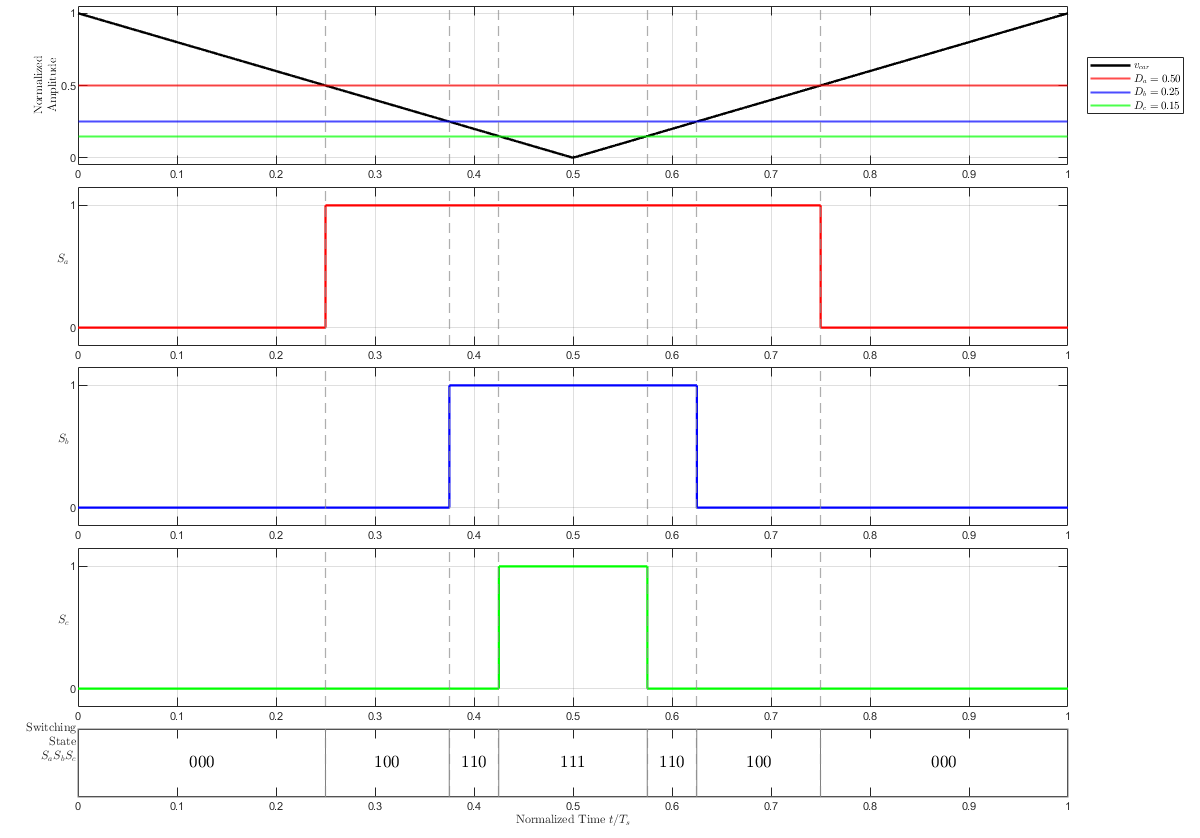
\includegraphics[width=0.8\linewidth]{center-aligned-pwm2.png}
    \caption{Three-Phase Center Aligned PWM}
    \label{fig:center-aligned-pwm2}
\end{figure}

The dwell times $T_1$, $T_2$ and $T_0$ specify the total duration for which the inverter must apply each voltage vector during a switching period. These quantities do not, however, directly correspond to the duty cycles applied to the individual inverter legs. To implement the desired switching sequence using a timer peripheral, the vector dwell times must first be converter into the total ON time of each high side switch.


%=========================================================================%
\paragraph{Modulation \& Duty Cycles}
\label{sec:space-vector-modulation}
%=========================================================================%

Consider the switching sequence for Sector 1. The active vectors are $\mathbf{V}_1=(100)$ and $\mathbf{V}_2=(110)$. The zero-vector dwell time $T_0$ is divided equally between the two zero states:

\begin{equation}
    T_{000} = T_{111} = \frac{T_0}{2}
\end{equation}

The ON-time of each inverter leg can therefore be determined by summing the dwell times of all switching states for which that leg is high. Considering the Sector 1 switching states:

\[
\begin{array}{c|c|c|ccc}
    \text{Vector} & \text{State} & \text{Total Dwell Time}
    & S_a & S_b & S_c \\
    \hline
    \mathbf{V}_0 & 000 & T_0/2 & 0 & 0 & 0 \\
    \mathbf{V}_1 & 100 & T_1   & 1 & 0 & 0 \\
    \mathbf{V}_2 & 110 & T_2   & 1 & 1 & 0 \\
    \mathbf{V}_7 & 111 & T_0/2 & 1 & 1 & 1
\end{array}
\]

The phase-$a$ inverter leg is high during $\mathbf{V}_1$, $\mathbf{V}_2$, and $\mathbf{V}_7$. The phase-$b$ leg is high during $\mathbf{V}_2$ and $\mathbf{V}_7$, while the phase-$c$ leg is high only during $\mathbf{V}_7$. Thus:

\begin{align}
    T_a &= T_1 + T_2 + \frac{T_0}{2}, \\
    T_b &= T_2 + \frac{T_0}{2}, \\
    T_c &= \frac{T_0}{2}
\end{align}

The corresponding PWM duty cycles are obtained by dividing each phase ON-time by the switching period:

\begin{equation}
    D_a = \frac{T_a}{T_s}, \qquad
    D_b = \frac{T_b}{T_s}, \qquad
    D_c = \frac{T_c}{T_s}
\end{equation}

Therefore, for Sector 1:

\begin{equation}
    D_a = \frac{T_1 + T_2 + T_0/2}{T_s}, \qquad
    D_b = \frac{T_2 + T_0/2}{T_s}, \qquad
    D_c = \frac{T_0/2}{T_s} \qquad
\end{equation}

The same procedure can be repeated for each of the remaining sectors. The resulting duty cycles are summarized in Table \ref{tab:svpwm-duty-cycles}.

\begin{table}[H]
    \centering
    \caption{SVPWM phase duty cycles for each sector.}
    \label{tab:svpwm-duty-cycles}
    \renewcommand{\arraystretch}{2.1}
    \begin{tabular}{c|c|c|c}
        \hline
        \textbf{Sector}
        & $\boldsymbol{D_a}$
        & $\boldsymbol{D_b}$
        & $\boldsymbol{D_c}$ \\
        \hline

        1 &
        $\dfrac{T_1+T_2+T_0/2}{T_s}$ &
        $\dfrac{T_2+T_0/2}{T_s}$ &
        $\dfrac{T_0/2}{T_s}$ \\

        2 &
        $\dfrac{T_1+T_0/2}{T_s}$ &
        $\dfrac{T_1+T_2+T_0/2}{T_s}$ &
        $\dfrac{T_0/2}{T_s}$ \\

        3 &
        $\dfrac{T_0/2}{T_s}$ &
        $\dfrac{T_1+T_2+T_0/2}{T_s}$ &
        $\dfrac{T_2+T_0/2}{T_s}$ \\

        4 &
        $\dfrac{T_0/2}{T_s}$ &
        $\dfrac{T_1+T_0/2}{T_s}$ &
        $\dfrac{T_1+T_2+T_0/2}{T_s}$ \\

        5 &
        $\dfrac{T_2+T_0/2}{T_s}$ &
        $\dfrac{T_0/2}{T_s}$ &
        $\dfrac{T_1+T_2+T_0/2}{T_s}$ \\

        6 &
        $\dfrac{T_1+T_2+T_0/2}{T_s}$ &
        $\dfrac{T_0/2}{T_s}$ &
        $\dfrac{T_1+T_0/2}{T_s}$ \\

        \hline
    \end{tabular}
\end{table}

This implementation of SVPWM provides a useful geometric interpretation of how the inverter synthesizes a commanded voltage vector as the time averaged combination of adjacent inverter state vectors within a sector. While this approach clearly shows how the commanded voltage vector is produced by the inverter switching states, it requires determining the current sector and using different dwell-time equations for each phase depending on the sector. Fortunately, the same SVPWM duty cycles can be obtained without explicitly calculating sectors or vector dwell times, as shown in the following section.


%=========================================================================%
\subsubsection{Common-Mode Injection SVPWM}
\label{sec:common-mode-injection-svpwm}
%=========================================================================%

By injecting a zero-sequence voltage, the three phase-voltage commands can instead be shifted within the available DC-link voltage range, providing a considerably simpler implementation of SVPWM.

Consider the three sinusoidal commanded phase voltages:

\begin{equation}
    v_{an}^* = V_m\cos(\theta_e)
\end{equation}

\begin{equation}
    v_{bn}^* = V_m\cos(\theta_e - \frac{2\pi}{3})
\end{equation}

\begin{equation}
    v_{cn}^* = V_m\cos(\theta_e + \frac{2\pi}{3})
\end{equation}

Where:

\begin{equation}
    V_m = \sqrt{(v_\alpha^*)^2 + (v_\beta^*)^2}
\end{equation}

Which may be obtained ufrom the commanded $\alpha\beta$ frame voltage vector through the inverse Clarke transform:

\begin{equation}
    \begin{bmatrix}
        v_a^* \\
        v_b^* \\
        v_c^*
    \end{bmatrix}
    =
    \begin{bmatrix}
        1 & 0 \\
        -\frac{1}{2} & \frac{\sqrt{3}}{2} \\
        -\frac{1}{2} & -\frac{\sqrt{3}}{2}
    \end{bmatrix}
    \begin{bmatrix}
        v_\alpha^* \\
        v_\beta^*
    \end{bmatrix}
\end{equation}

At any instant, the maximum and minimum of the three-phase voltage commands can be found as:

\begin{align}
    v_{max} &= \max(v_a^*, v_b^*, v_c^*), \\[6pt]
    v_{min} &= \min(v_a^*, v_b^*, v_c^*)
\end{align}

The midpoint between these two values is:

\begin{equation}
    v_{mid} = \frac{v_{max} + v_{min}}{2}
\end{equation}

Recall the equation for inverter pole voltage:

\begin{equation}
    v_{xg} = v_{xn} + v_{ng}
\end{equation}

Since a two-level inverter can only output voltages between its supply voltage and reference:

\[
    0 \leq V_{xg} \leq V_{DC}
\]

The commanded pole voltages are first shifted upwards by half the DC-bus voltage, as with SPWM and THI. However, in common-mode injected SVPWM, an additional term is subtracted from all three pole-voltage commands. This term is the midpoint between the instantaneous maximum and minimum phase-voltage commands, such that the resulting pole-voltage commands have equal margin from the upper and lower limits of the DC bus for every instantaneous command. Since the this assumes a balanced, three phase system, and because the same offset is applied to all three pole-voltage commands, this represents a common-mode voltage. Therefore:

\begin{equation}
    v_{cm}^* = \frac{V_{DC}}{2} - \frac{v_{max} + v_{min}}{2}
\end{equation}

We have extensively explored in Section \ref{sec:common-mode-voltage-injection} how we are free to select and inject a common-mode voltage into the commanded inveter pole voltages. This has no effect on the final phase and line voltages that the motor is provided. Recall that this is because the phase voltage is the difference between the pole and neutral voltages. For balanced sinusoidal phase voltages, the neutral voltage is equal to the common-mode voltage. Therefore, since we have shifted both the pole and neutral voltages by the same amount, the common-mode component cancels in the phase voltage. From Section \ref{sec:common-mode-voltage-injection}:

\begin{equation}
    v_{ag}^* = v_{an}^* + v_{cm}^*, \qquad
    v_{bg}^* = v_{bn}^* + v_{cm}^*, \qquad
    v_{cg}^* = v_{cn}^* + v_{cm}^*
\end{equation}

Where the average neutral voltage is approximately equal to the commanded common-mode voltage:

\begin{equation}
    \overline{v}_{ng} \approx v_{cm}^*
\end{equation}

Substituting for the common-mode voltage:

\begin{equation}
    v_{ag}^* = v_{an}^* + \frac{V_{DC}}{2} - \frac{v_{max} + v_{min}}{2}
\end{equation}

\begin{equation}
    v_{bg}^* = v_{bn}^* + \frac{V_{DC}}{2} - \frac{v_{max} + v_{min}}{2}, \qquad
\end{equation}

\begin{equation}
    v_{cg}^* = v_{cn}^* + \frac{V_{DC}}{2} - \frac{v_{max} + v_{min}}{2}
\end{equation}

Then, since the average pole voltage produced by PWM is:

\begin{equation}
    v_{xg} = D_xV_{DC}
\end{equation}

\begin{equation}
    D_a = \frac{1}{2} + \frac{v_{an}^* - \frac{1}{2}(v_{max} + v_{min})}{V_{DC}}
\end{equation}

\begin{equation}
    D_b = \frac{1}{2} + \frac{v_{bn}^* - \frac{1}{2}(v_{max} + v_{min})}{V_{DC}}
\end{equation}

\begin{equation}
    D_c = \frac{1}{2} + \frac{v_{cn}^* - \frac{1}{2}(v_{max} + v_{min})}{V_{DC}}
\end{equation}

This implementation produces the same centered PWM duty cycles as the sector-based SVPWM method, but avoids explicit sector identification and dwell-time calculations. Instead, the phase-voltage commands are shifted by a common-mode component determined only by their instantaneous maximum and minimum values. This makes the common-mode injection method particularly convenient for digital implementation, requiring only an inverse Clarke transformation, maximum and minimum comparisons, and the calculation of the three phase duty cycles.

From these duty cycles, we can again arrive at the $V_{DC}/\sqrt{3}$ limit of SVPWM for a rotating vector of constant magnitude. Consider the duty cycle of an arbitrary phase:

\begin{equation}
    D_x = \frac{1}{2} + \frac{v_x^* - \frac{1}{2}(v_{max} + v_{min})}{V_{DC}}
\end{equation}

At the maximum duty cycle, $v_x^*$ will be at a maximum:

\begin{equation}
    D_{max} = \frac{1}{2} + \frac{v_{max} - v_{min}}{2V_{DC}}
\end{equation}

Likewise:

\begin{equation}
    D_{min} = \frac{1}{2} - \frac{v_{max} - v_{min}}{2V_{DC}}
\end{equation}

By definition:

\begin{equation}
    0 \leq D_x \leq 1
\end{equation}

Therefore:

\begin{equation}
    D_{max} \leq 1
\end{equation}

Requires:

\begin{equation}
    \frac{1}{2} + \frac{v_{max} - v_{min}}{2V_{DC}} \leq 1
\end{equation}

Giving:

\begin{equation}
    v_{max} - v_{min} \leq V_{DC}
\end{equation}

Therefore, we must find the largest instantaneous difference between the maximum and minimum of three balanced sinusoids of amplitude, $V_m$. Since the difference between any two phase commands is the line-to-line voltage:

\begin{equation}
    v_a^* - v_b^* = \sqrt{3}V_m\cos(\theta_e + \frac{\pi}{6})
\end{equation}

Its maximum magnitude is therefore $\sqrt{3}V_m$. Consequently:

\[
    \underset{\theta_e}{\max}(v_{max} - v_{min}) = \sqrt{3}V_m
\]

However, SVPWM requires that:

\begin{equation}
    v_{max} - v_{min} \leq V_{DC}
\end{equation}

Therefore:

\begin{equation}
    \sqrt{3}V_m \leq V_{DC}
\end{equation}

And finally:

\begin{equation}
    V_m \leq \frac{V_{DC}}{3}
\end{equation}


%=========================================================================%
\subsubsection{Practical Implementation of SVPWM}
\label{sec:practical-implementation-of-svpwm}
%=========================================================================%

The common-mode injection method provides a relatively simple implementation of SVPWM. The controller first receives the commanded stationary-frame voltage vector $v_\alpha^*$ and $v_\beta^*$, which is converted into the three commanded phase voltages using the inverse Clarke transformation:

\begin{equation}
    \mathbf{v}_{abc}^* = \mathbf{T}_c^{-1}\mathbf{v}_{\alpha\beta}^*
\end{equation}

The instantaneous maximum and minimum phase voltage commands are then determined:

\begin{equation}
    v_{max} = \max(v_{an}^*, v_{bn}^*, v_{cn}^*), \qquad
    v_{min} = \min(v_{an}^*, v_{bn}^*, v_{cn}^*)
\end{equation}

From which their midpoint is calculated as:

\begin{equation}
    v_{mid} = \frac{v_{max} - v_{min}}{2}
\end{equation}

The three inverter duty cycles can then be calcualted 

\begin{equation}
    D_a = \frac{1}{2} + \frac{v_{an}^* - \frac{1}{2}(v_{max} + v_{min})}{V_{DC}}
\end{equation}

\begin{equation}
    D_b = \frac{1}{2} + \frac{v_{bn}^* - \frac{1}{2}(v_{max} + v_{min})}{V_{DC}}
\end{equation}

\begin{equation}
    D_c = \frac{1}{2} + \frac{v_{cn}^* - \frac{1}{2}(v_{max} + v_{min})}{V_{DC}}
\end{equation}

This implementation represents the final result that this chapter has been working toward. Beginning with the three-phase inverter and its discrete switching states, the voltage space vector was developed and used to introduce SPWM, third-harmonic injection, and finally SVPWM. Unlike SPWM and THI, SVPWM does not require the explicit generation of sinusoidal phase-voltage references. Instead, it can directly receive the commanded stationary-frame voltage vector $v_\alpha^*,v_\beta^*$, convert it into instantaneous phase-voltage commands through the inverse Clarke transformation, and calculate the inverter duty cycles using the common-mode injection method. SVPWM therefore provides a direct interface between a commanded voltage vector and the physical inverter switching signals required to produce it. The remaining question is how the commanded voltage vector itself should be determined. This is the focus of the next chapter, where Field-Oriented Control (FOC) is developed to calculate the voltage commands required to control the PMSM's currents, torque, and magnetic field.


%=========================================================================%
\pagebreak
\section{Field Oriented Control}
\label{sec:field-oriented-control}

\subsection{Principles of Field Oriented Control}
\label{sec:principles-field-oriented-control}

\subsubsection{From Three-Phase Currents to Flux \& Torque}
\label{sec:three-phase-currents-to-flux-and-torque}
%=========================================================================%

The previous chapter established how a desired stator voltage vector can be synthesized by the three-phase inverter using SVPWM, among other modulation techniques. Given a commanded stationary frame voltage vector, $\mathbf{v}_{\alpha\beta}^*$, SVPWM determins the inverter switching states and their corresponding duty cycles required to appoximate that vector over each switching period. The remaining problem to be solved is therefore not how to produce a voltage vector, but rather which voltage vector should be commanded in order to produce the desired behaviour of the motor.

For a PMSM, the quantites of primary interest are generally not the stator voltages themselves. Instead, the objective is to control the electromagnetic torque developed by the machine, and through it, the rotor speed or position. As established in Chapter \ref{sec:mathematical-model-of-pmsms}, the electromagnetic torque is determined by the interaction between the rotor magnetic field and the magnetic field produced by the stator currents. Consequently, precise control of the motor ultimately requires preceise control of the magnitude and orientation of the stator current vector relative to the rotor.

Attempting to perform this control directly using the three phase currents, $i_a$, $i_b$, and $i_c$ is inconvenient. Under balanced sinusoidal operation, each phase current is continuously varying with electrical angle:

\begin{align}
    i_a &= I_m\cos(\theta_e + \phi) \\
    i_b &= I_m\cos(\theta_e + \phi - \frac{2\pi}{3}) \\
    i_c &= I_m\cos(\theta_e + \phi + \frac{2\pi}{3})
\end{align}

Such that even steady-state operating requires the controller to track three time-varying reference quantities, like in SPWM. Furthermore, the three currents are not independent: for a balanced three-phase machine:

\begin{equation}
    i_a + i_b + i_c = 0
\end{equation}

The physical quanity of interest is therefore better understood not as three indpenedent phase currents, but as a single stator current vector rotating within the machine.

The Clarke transofrm developed in Chapter \ref{sec:mathematical-model-of-pmsms} provides the first simplification by expressing this three-phase system using two orthogonal station-frame components, $i_\alpha$, and $i_\beta$. These components describe the same stator current vector:

\begin{equation}
    \mathbf{i}_s = i_a\hat{a} + i_b\hat{b} + i_c\hat{c} = i_\alpha\hat{\alpha} + i_\beta\hat{\beta}
\end{equation}

The current vector, however, continues to rotate through the stationary $\alpha\beta$ reference frame as the machine operates. Thus, although the representation has been reduced from three dimensions to two, the quantites being controlled remain time-varying.

The central idea of Field-Oriented Control (FOC) is to remove this remaining rotation by observing the stator current vector from a reference frame that rotates with the rotor magnetic field. Applying the Park transformation using the rotor electrical angle $\theta_e$ rotates the stationary-frame quantities into the synchronous $dq$ reference frame.

Using typical conventions, the $d$-axis is chosen to remain aligned with the rotor permanent-magnet flux, while the $q$-axis remains $90^\circ$ electrical ahead of it. Consequently, a stator current vector rotating synchronously with the rotor appears stationary when viewed from this reference frame which rotates at the same rate. Balanced sinusoidal phase currents that continuously vary in the $abc$ and $\alpha\beta$ frames therefore become approximately constant, DC quantities $i_d$ and $i_q$ under steady-state synchronous operation. 

This change of reference frame is what makes FOC particularly powerful. Rather than forcing a feedback controller to track sinusoidal quantities whose frequency changes with rotor speed, the controller can regulate approximately DC quantities. More importantly, the orientation of the $dq$ frame gives these quantities a direct physical interpretation. The $d$-axis current determins the component of stator flux magnetomotive force aligned with the rotor magnetic field, while the $q$-axis current determines the component perpendicular to it, which we have seen is directly proportional to torque. The stator current is then equivalently written as:

\begin{equation}
    \mathbf{i}_s = i_d\hat{d} + i_q\hat{q}
\end{equation}

Where its magnitude and orientation relative to the rotor are given by:

\begin{equation}
    |\mathbf{i}_s| = \sqrt{i_d^2 + i_q^2}, \qquad
    \gamma = \tan^{-1}\left(\frac{i_q}{i_d}\right)
\end{equation}

Thus, regulating $i_d$ and $i_q$ is equivalent to regulating the magnitude and orientation of the stator magnetic field relative to the rotor. This relationship becomes particularly important when considering electromagnetic torque. For a PMSM, the $dq$-frame torque expression derived in Section \ref{sec:electromechanical-model} is:

\begin{equation}
    T_e = \frac{3}{2}p[\lambda_mi_q + (L_d - L_q)i_di_q]
\end{equation}

Where the first term represents torque produced through the interaction of the permanent magnet flux with the $q$-axis stator current, while the second represents reluctance torque resulting from rotor saliency. For a surface mount PMSM, where $L_d \approx L_q$, the reluctance torque negligble and the expression reduces to:

\begin{equation}
    T_e = \frac{3}{2}p\lambda_mi_q
\end{equation}

Electromagntic torque is then directly proportional to a single DC control variable, $i_q$. Meanwhile, $i_d$ determines the component of stator current directed along the rotor magnetic field. For an ideal, nonsalient PMSM operating below base speed, no additional $d$-axis current is generally required, and the reference may initially be chosen as:

\begin{equation}
    i_d^* = 0
\end{equation}

Under these conditions, commanding $i_q^*$ effectively commands motor torque while $i_d$ is independently regulated to zero. The original problem of controlling three sinusoidal phase currents has therefore been transformed into the considerably simpler problem of regulating two approximately constant orthogonal current components. 

This is the fundmental principle underlying field-oriented control. The measured phse currents are transformed into the rotating $dq$ reference frame, compared against desired $d$- and $q$- axis current references, and the resulting errors are used to determine the stator voltage vector required to drive the currents toward their commanded values. The commanded voltage vector is then transformed back into stationary and three-phase reference frames and synthesized by the inverter using the modulation techniques developed in Chapter \ref{sec:three-phase-interters-and-modulation-techniques}. 


%=========================================================================%
\subsubsection{Current Control Loop}
\label{sec:current-control-loop}
%=========================================================================%

The transformation of the stator currents into the rotor synchronous $dq$ frame provides a set of variables that are well suited for feedback control. Until this point, we have only examined simple open-loop implementations of PMSM control. Field Oriented Control requires a closed loop control system to regulate the measured $d$- and $q$-axis currents to their commanded values. The current control loop block diagram for FOC is shown in Figure \ref{fig:foc-block-diagram-v1}. In later sections, we will revisit this block diagram, adding to it as we increase the system performance and complexity.

\vspace{0.5cm}
\begin{figure}[htbp]
    \centering
    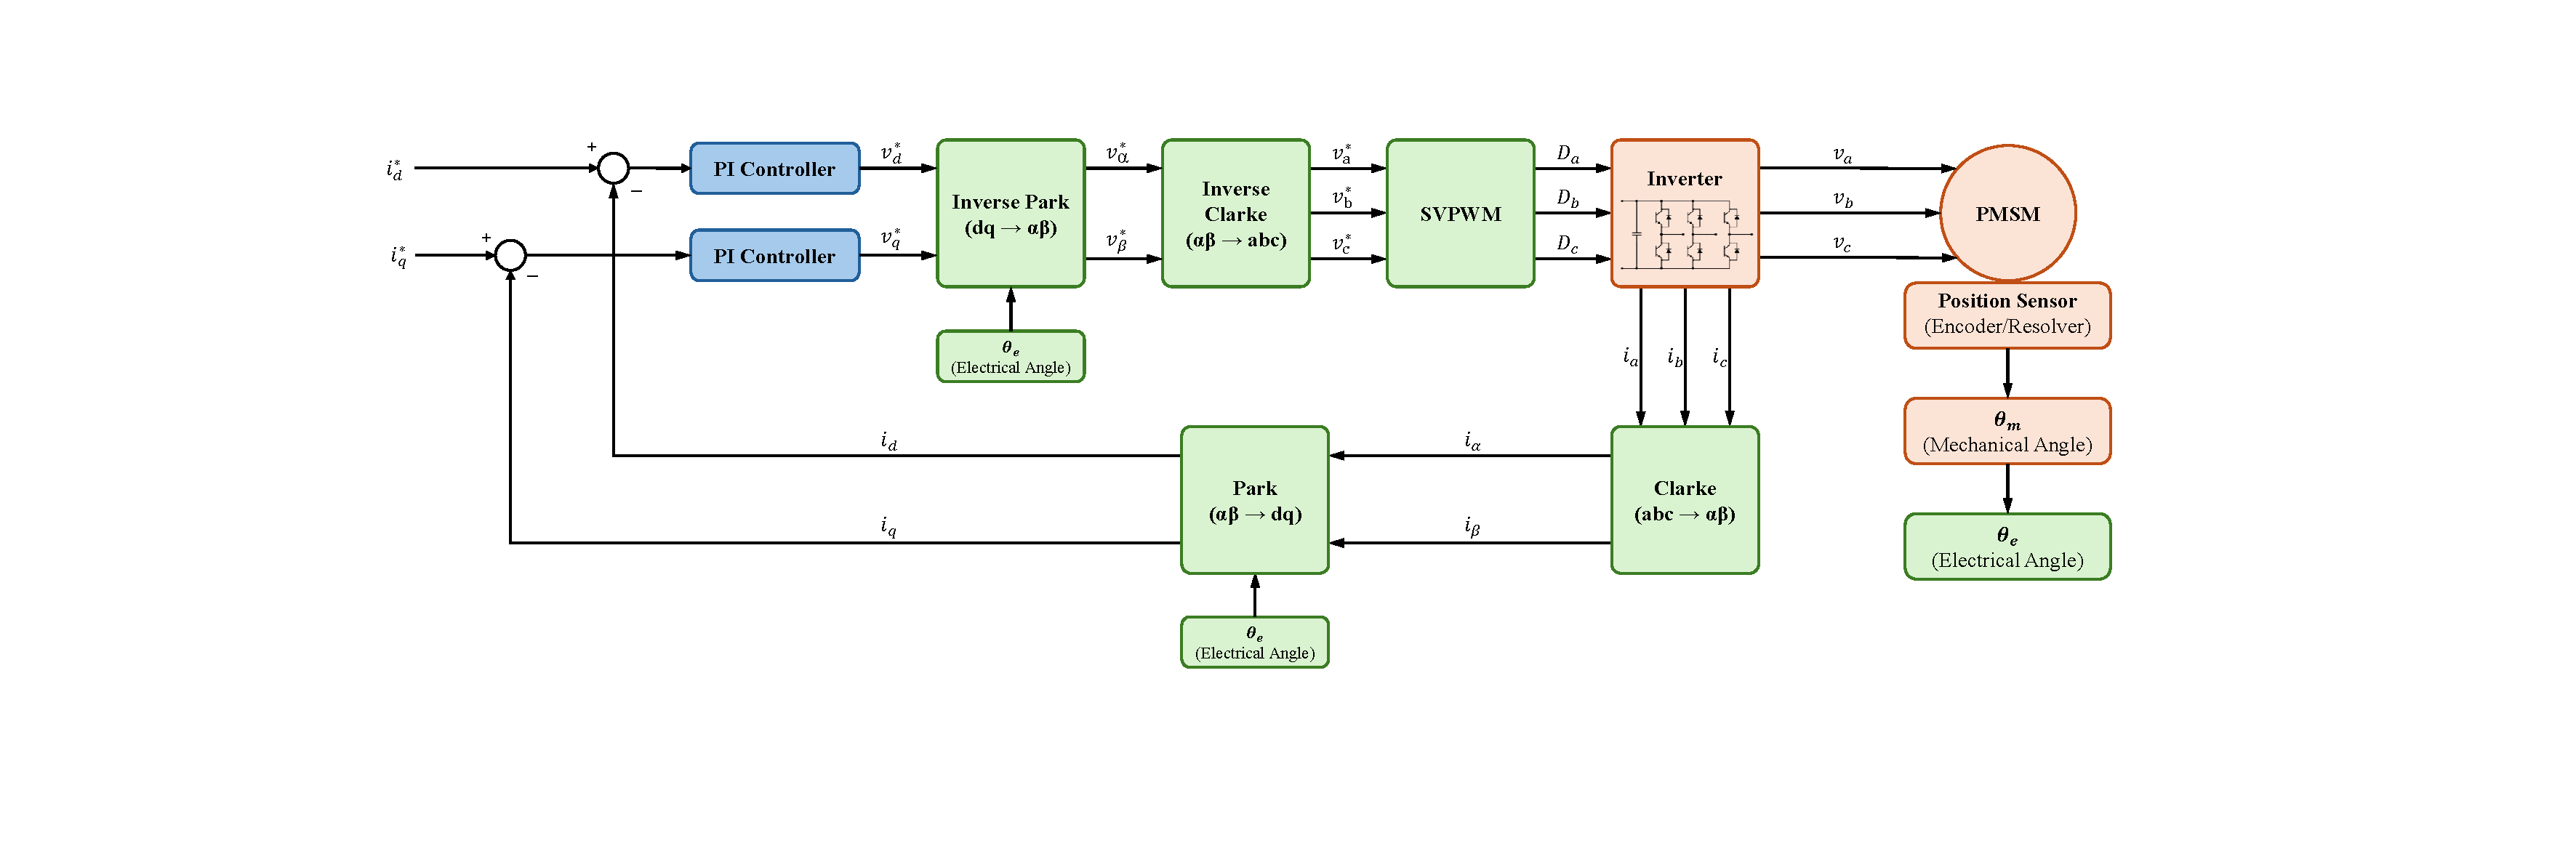
\includegraphics[
        width=\textwidth,
        keepaspectratio
    ]{foc-block-diagram-v1.pdf}

    \caption{Field Oriented Control Block Diagram}
    \label{fig:foc-block-diagram-v1}
\end{figure}

Beginning with the input of the control system, the desired operating condition of the motor is represented by the current references $i_d^*$ and $i_q^*$. These references spcify the desired components of the stator current vector relative to the rotor magnetic field. The measured currents $i_d$ and $i_q$ are subtracted from their respective references to form the current errors:

\begin{equation}
    e_d = i_d^* - i_d, \qquad
    e_q = i_q^* - i_q
\end{equation}

The objective of the current controllers is to drive these errors toward zero. Because the controlled variables are appoximately constant under steady-state operation, conventional proportional-integral (PI) controllers are well suited to this task. We will show this mathematically in later sections. In their most simple continuous-time form, the two controllers may be represented as:

\begin{equation}
    v_{d,PI}^* = K_{p,d}e_d + K_{i,d}\int e_d \space dt
\end{equation}

\begin{equation}
    v_{q,PI}^* = K_{p,q}e_q + K_{i,q}\int e_q \space dt
\end{equation}

Note that the controller outputs are voltage commands rather than current commands, while the input is the current error. This distrinction is fundamental to the operation of FOC. The inverter cannot directly impose a desired stator current; it can only apply voltages to the motor windings. The resulting currents are determined by the electrical dynamics of the machine. Consequently, the role of the current controller is to continuously determine the $dq$-axis voltages required to drive the measured currents toward their desired values.

In the simplified control architecture, these controller outputs are taken as the commanded synchronous-frame voltages:

\begin{equation}
    v_d^* \approx v_{d,PI}^*, \qquad
    v_q^* \approx v_{q,PI}^*
\end{equation}

We will later modify these values with feedforward terms to improve performance. The commanded voltage vector may therefore be expressed in the synchronous reference frame as:

\begin{equation}
    \mathbf{v}_{dq}^* = v_d^*\hat{\mathbf{d}} + v_q^*\hat{\mathbf{q}}
\end{equation}

Unlike the current-control calculations, however, the physical inverter is stationary with respect to the stator and cannot directly apply voltages along the rotating $d$- and $q$-axis. The commanded voltage vector must therefore be transformed back into a stationary reference frame before it can be synthesized by the inverter.

Using the measured or estimated rotor electrical angle $\theta_e$, the inverse Park transformation rotates the commanded voltage vector from the synchronous $dq$ frame into the stationary $\alpha\beta$ frame:

\begin{equation}
    \mathbf{v}_{\alpha\beta}^* = \mathbf{T}_p^{-1}\mathbf{v}_{dq}^*
\end{equation}

The resulting quantities $v_\alpha^*$ and $v_\beta^*$ describe the desired stator voltage vector in stationary coordinates. As developed in Chapter 2, this voltage vector can be supplied directly to the sector based SVPWM algorithm to determine the required inverter duty cycles. Alternatively, an inverse Clarke transformation may be used to express the voltage command as the the equivalent three-phase references, $v_a^*$, $v_b^*$ and $v_c^*$ if SVPWM is used.

\begin{equation}
    \mathbf{v}_{abc}^* = \mathbf{T}_c^{-1}\mathbf{v}_{\alpha\beta}^*
\end{equation}

The inverter then applies the corresponding phase voltages, $v_a$, $v_b$ and $v_c$ to the stator windings in terms of duty cycles. These voltages cause the phase currents to evolve according to the electrical dynamics of the PMSM. The resulting currents $i_a$, $i_b$ and $i_c$ are measured and returned to the controller, closing the feedback loop.

To compare the measured currents against the synchronous frame references, the measurement process performs the reverse sequence of coordinate transformations. The measured phase currents are first transformed into the stationary reference frame using the Clarke transformation:

\begin{equation}
    \mathbf{i}_{\alpha\beta} = \mathbf{T}_c\mathbf{i}_{abc}
\end{equation}

Then are subsequently rotated into the synchronous reference frame using the Park transformation:

\begin{equation}
    \mathbf{i}_{dq} = \mathbf{T}_p\mathbf{i}_{abc}
\end{equation}

The same electrical rotor angle $\theta_e$ must therefore be used consistently by both the forward and inverse transformations. For a sensored FOC system, this angle may be obtainred from an encoder or resolver measuring the mechancial rotor angle $\theta_m$, from which the electrical angle is determined according to:

\begin{equation}
    \theta_e = p\theta_m
\end{equation}

Where $p$ is the number of pole pairs. In practice, an appropriate electrical zero angle offset must also be established so that the controller's $d$-axis is correctly aligned with the permamnent magnet flux axis. Sensorless control replaces the physical position measurement with an estimate of this angle, but otherwise retains the same fundamental reference-frame structure.

Once transformed, $i_d$ and $i_q$ are again compared with $i_d^*$ and $i_q^*$ and the process repeats. Although several transformations are involved, the control objective itself is straightforward: adjust the stator voltage vector such that the measured synchronous frame current vector follows its commanded value. 


%=========================================================================%
\subsection{Design of \texorpdfstring{$dq$}{dq} Current Controllers}
\label{sec:design-of-dq-current-controllers}
%=========================================================================%

The current-control structure of Section \ref{sec:current-control-loop} establishes the basic feedback architecture of Field-Oriented Control. The measured $d$- and $q$-axis currents are compared against their respective reference values, and the resulting current errors are minmimized by feedback controllers through the commanded $dq$ reference frame voltages. However, Figure \ref{fig:foc-block-diagram-v1} alone does not establish how these controllers should be designed, nor does it account for the dynmaic relationship between the commanded voltages and resulting stator currents.

To design the current controllers systematically, the PMSM iteself must be considered as part of the control loop. From a tradtitional control system persepective, the motor acts as the plant: the commanded stator voltages $v_d^*$ and $v_q^*$ form the plant inputs, while the resulting currents $i_d$ and $i_q$ form the quantities to be regulated. However, inspection of the PMSM voltge equations reveals a problem--The two axes are dynamically coupled through terms proportional to the electrical speed. In addition, the $q$-axis voltage must overcome the back-EMF produced by the rotor flux.

Consequently, the PMSM cannot be treated as two independent $RL$ circuits, making the process of tuning the PI current controllers significantly more difficult. This section develops the $dq$-axis current controllers beginning from the coupled PMSM model. We will see how we can eliminate the cross coupling terms and approximatley decouple the two axes. The resulting system can be used to derive the gains of the $dq$-axis current controllers. 


%=========================================================================%
\subsubsection{Coupled \texorpdfstring{$dq$}{dq}-Axis Dynamics}
\label{sec:coupled-dq-dynamics}
%=========================================================================%

Recall the PMSM motor equations derived in Chapter \ref{sec:mathematical-model-of-pmsms}:

\begin{equation}
    v_d = R_si_d + L_d\frac{di_d}{dt} - \omega_eL_qi_q
\end{equation}

\begin{equation}
    v_q = R_si_q + L_q\frac{di_q}{dt} + \omega_eL_di_d + \omega_e\lambda_m
\end{equation}

These equations describe how the applied $dq$ voltages determine the evolution of the corresponding stator currents. Rearranging each equation to isolate the current derivative:

\begin{equation}
    L_d\frac{di_d}{dt} = v_d - R_si_d + \omega_eL_qi_q
\end{equation}

\begin{equation}
    L_q\frac{di_q}{dt} = v_q - R_si_q - \omega_eL_di_d - \omega_e\lambda_m
\end{equation}

If  the speed dependent terms were absent, each axis would have the form of a simple series $RL$ circuit. Consider briefly, for example, the $d$-axis dynamics would reduce to:

\begin{equation}
    v_d = R_si_d + L_d\frac{di_d}{dt}
\end{equation}

Taking the Laplace transform with zero inital conditions:

\begin{equation}
    V_d(s) = (R_s + sL_d)I_d(s)
\end{equation}

The corresponding voltage to current transfer function is then:

\begin{equation}
    G_d(s) = \frac{I_d(s)}{V_d(s)} = \frac{1}{L_ds + R_s}
\end{equation}

Similarly, the $q$-axis plant would be:

\begin{equation}
    G_q(s) = \frac{I_q(s)}{V_q(s)} = \frac{1}{L_qs + R_s}
\end{equation}

%=========================================================================%
\subsubsection{Coupled \texorpdfstring{$dq$}{dq}-Axis Current Dynamics}
\label{sec:coupled-dq-axis-current-dynamics}
%=========================================================================%

Recall from Section \ref{sec:electromechanical-model} that the PMSM's stator voltage equations in the synchronous $dq$ frame are described by:

\begin{equation}
    v_d = Ri_d + L_d\frac{di_d}{dt} - \omega_eL_qi_q
\end{equation}

\begin{equation}
    v_q = Ri_q + L_q\frac{di_q}{dt} + \omega_eL_di_d
\end{equation}

These equations describe how the applied $d$- $q$-axis voltages determine the evolution of the corresponding stator currents. If the speed-dependent terms were absent, each axis would have the form of a simple series $RL$ circuit. For example, the $d$-axis current dynamics would reduce to:

\begin{equation}
    v_d = Ri_d + L_d\frac{di_d}{dt}
\end{equation}

Taking the laplace transform with zero initial conditions:

\begin{equation}
    V_d(s) = (R + sL_d)I_d(s)
\end{equation}

The correspond voltage-to-current transfer function is therefore:

\begin{equation}
    \frac{I_d(s)}{V_d(s)} = \frac{1}{R + sL_d} = \frac{1/R}{1 + sL_d/R}
\end{equation}

Similarly, the $q$-axis current dynamics would be:

\begin{equation}
    \frac{I_q(s)}{V_q(s)} = \frac{1}{R + sL_q} = \frac{1/R}{1 + sL_q/R}
\end{equation}

The first order plants are particularly convenient for current-controller design for two primary reasons. First, as a first order system, the plant has a single pole and no zeros. This makes it particularly well suited to PI control, which results in zero steady state error. 

Second, both axes are decoupled, meaning that the $d$-axis current is determined only by the $d$-axis voltage, and the $q$-axis current is determined only by the $q$-axis voltage. This allows each axis to be controlled independently, with a single PI controller for each axis.

However, as shown above, the complete PMSM equations contain additional terms that prevent the two axes from behaving independently. In the $d$-axis equation, the term:

\begin{equation}
    -\omega_eL_qi_q
\end{equation}

Represents a voltage induced on the $d$-axis as a consequence of $q$-axis current and rotation of the reference frame. Similarly, the $q$-axis equation contains the cross-coupling term:

\begin{equation}
    \omega_eL_di_d
\end{equation}

As well as the permanent-magnet back-EMF term:

\begin{equation}
    \omega_e\lambda_m
\end{equation}

The magnitude of each term increases with electrical speed, $\omega_e$. At low speeds, these terms are small and the $dq$-axis current dynamics are approximately decoupled. However, as speed increases, the cross-coupling terms become significant and the controller must compensate for these distrubances.

A more useful control structure can be obtained by explicitly compensating for these known terms. By incorporating the cross-coupling and permanent-magnet back-EMF voltages into the commanded voltage vector as feedforward terms, the remaining dynamics seen by the feedback controllers can be made to approximately resemble the independent $RL$ plants derived above. This process is referred to as $dq$-axis decoupling.


%=========================================================================%
\subsubsection{Axis Decoupling and Feedforward Compensation}
\label{sec:axis-decoupling-ff-compensation}
%=========================================================================%

Rather than requiring the PI controllers to reject the predictable cross-coupling and back-EMF terms as disturbances, these terms can be added to the commanded voltage vector as feedforward compensation.

The commanded $dq$-axis voltage is therefore separated into two components: a feedback component generated by the PI controllers, and a feedforward component calculated from the PMSM model. If we denote the feedforward terms as:

\begin{equation}
    v_{d,ff} = -\omega_eL_qi_q
\end{equation}

And:

\begin{equation}
    v_{q,ff} = \omega_eL_di_d + \omega_e\lambda_m
\end{equation}

Then, before the application of the park transform, we inject these feedforward terms into the commanded PI voltages:

\begin{equation}
    v_d^* = v_{d,PI}^* - \omega_eL_qi_q
\end{equation}

\begin{equation}
    v_q^* = v_{q,PI}^* + \omega_eL_di_d + \omega_e\lambda_m
\end{equation}

If we substitute these expressions into the PMSM voltage equations, we can see that the cross-coupling and back-EMF terms are cancelled, leaving the PI controllers to regulate the currents through approximately decoupled first-order plants. For the $d$-axis:

\begin{align}
    v_d^* &= R_si_d + L_d\frac{di_d}{dt} - \omega_eL_qi_q \\
    v_{d,PI}^* - \omega_eL_qi_q &= R_si_d + L_d\frac{di_d}{dt} - \omega_eL_qi_q \\
    v_{d,PI}^* &= R_si_d + L_d\frac{di_d}{dt}
\end{align}

Similarly, for the $q$-axis:

\begin{align}
    v_q^* &= R_si_q + L_q\frac{di_q}{dt} + \omega_eL_di_d + \omega_e\lambda_m \\
    v_{q,PI}^* + \omega_eL_di_d + \omega_e\lambda_m &= R_si_q + L_q\frac{di_q}{dt} + \omega_eL_di_d + \omega_e\lambda_m \\
    v_{q,PI}^* &= R_si_q + L_q\frac{di_q}{dt}
\end{align}

%=========================================================================%
\subsubsection{Axis Decoupling \& Feedforard Compensation}
\label{sec:axis-decoupling-and-ff-compensation}
%=========================================================================%


%=========================================================================%
\subsubsection{PI Current Controller Design}
\label{sec:pi-current-controller-design}
%=========================================================================%


%=========================================================================%
\subsection{Voltage Limitations \& Anti-Windup}
\label{sec:voltage-limitations-and-anti-windup}
%=========================================================================%


-3.3.1 Voltage Vector Saturation
-3.3.2 PI Integrator Windup
-3.3.3 Anti-Windup Strategies

-3.4 Cascaded Torque, Velocity, and Position Control
-3.4.1 Torque Control
-3.4.2 Velocity Control
-3.4.3 Position Control

-3.5 Digital Implmentations of FOC
-3.5.1 Sampling the Control System
-3.5.2 Discreization of the PI Controller
-3.5.3 z-Domain Representation
-3.5.4 Computational Delay
-3.5.5 FOC Execution Sequence

-3.6 Rotor Position and Speed Feedback
-3.6.1 Sensored Rotor Position

-3.7 Sensorless Field Oriented Control
-3.7.1 Sensorless Control problem
-3.7.2 Back EMF Based Estiamtion
-3.7.3 Flux Observers
-3.7.4 State Observers
-3.7.5 Sliding Mode Observer
-3.7.6 PLL Based Angle Tracking
-3.7.7 Low Speed and Zero-Speed Limitations
%}




%=========================================================================%
\appendix
\renewcommand{\thesection}{\Alph{section}.}
%=========================================================================%

\section{Optimization of Third Harmonic Injection}
\label{app:thi-optimiazation}

This appendix section derives the optimal amplitude of the third harmonic component used in third-harmonic injection (THI). The objective is to determine the injection amplitude that minimizes the peak magnitude of the resulting phase-voltage reference for a given fundamental amplitude. Minimizing this peak allows the fundamental component to be maximized while keeping the commanded inverter pole voltages within the DC-bus limits. The derivation shows that this occurs when the third-harmonic amplitude is one-sixth of the fundamental amplitude and opposite in sign. 

Take the commanded phase-$a$ reference voltage:

\begin{equation}
    v_{ag}^* = \frac{V_{DC}}{2} + V_m\cos\theta_e + V_3\cos3\theta_e
\end{equation}

Since $V_{DC}/2$ is a DC offset, the maximum sinusoidal swing about the midpoint of the DC bus is determined entirely by the AC component. If we define $f(\theta_e)$ as:

\begin{equation}
    f(\theta) = V_m\cos\theta + V_3\cos3\theta
\end{equation}

To reduce the amplitude of the fundamental, the third harmonic is chosen opposite in sign to the fundamental near its peak. If we define:

\begin{equation}
    V_3 = -kV_m, \qquad
    k \geq 0
\end{equation}

Then:

\begin{equation}
    f(\theta) = V_m(\cos\theta - k\cos3\theta)
\end{equation}

Since $V_m$ scales the entire waveform, define the normalized reference:

\begin{equation}
    F(\theta) = \frac{f(\theta)}{V_m} = \cos\theta - k\cos3\theta
\end{equation}

The objective is to determine $k$ such that the maximum magnitude of the normalize reference is minimized:

\begin{equation}
    \underset{k}{min}\left[ \underset{\theta}{\max}|F(\theta)| \right]
\end{equation}

This minimizes the required inverter pole voltage swing for a given fundamental amplitude, $V_m$. To determine the extrema of the waveform, we differentiate with respect to $\theta$:

\begin{equation}
    F'(\theta) = -\sin\theta + 3k\sin3\theta
\end{equation}

At a maximum:

\begin{equation}
    -\sin\theta + 3k\sin3\theta = 0
\end{equation}

Using the identity:

\begin{equation}
    \sin3\theta = 3\sin\theta - 4\sin^3\theta
\end{equation}

Collecting terms:

\begin{equation}
    \sin\theta[-1 + 9k -12k\sin^2\theta] = 0
\end{equation}

Hence, one set of extreme occurs at:\

\begin{equation}
    \sin\theta = 0
\end{equation}

Additional extrema satisfy:

\begin{equation}
    -1 + 9k - 12k\sin^2\theta = 0
\end{equation}

Therefore:

\begin{equation}
\label{eqn:max-locations}
    \sin^2\theta = \frac{9k - 1}{12k}
\end{equation}

This equation only locates the off center extrema for a given $k$. These additional extrema exist only when:

\begin{equation}
    9k - 1 \geq 0
\end{equation}

Or:

\begin{equation}
    k \geq \frac{1}{9}
\end{equation}

Thus, $k = 1/9$ represents the point at which the original peak at $\theta = 0$ becomes locally flat and begins to split into two off center extrema. It does not, however, represent the minimum possible global peak. The effect of different $k$ values is illustrated in Figure \ref{fig:thi-k-values}.

\begin{figure}[H]
    \centering
    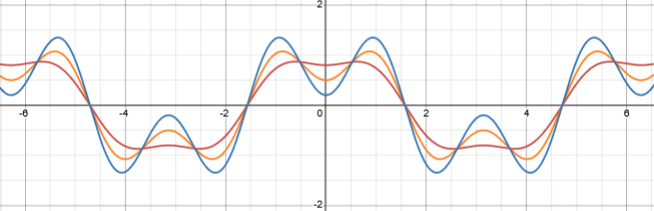
\includegraphics[width=0.75\linewidth]{thi-k-values.png}
    \caption{$f(\theta)$ for $k = 0.2$ (Red), $k = 0.5$ (Orange), $k = 0.8$ (Blue)}
    \label{fig:thi-k-values}
\end{figure}

To determine the value of $k$ that minimizes these new peaks, we begin with the triple angle identity. Recall $F(\theta)$:

\begin{equation}
    F(\theta) = \cos\theta - k\cos3\theta
\end{equation}

The triple angle identity is:

\begin{equation}
    \cos3\theta = 4\cos^3\theta - 3\cos\theta
\end{equation}

Let:

\begin{equation}
    x = \cos\theta
\end{equation}

Then:

\begin{align}
    F(x) &= x - k(4x^3 - 3x) \\
    &= (1 + 3k)x - 3kx^3
\end{align}

Differentiating with respect to $x$:

\begin{equation}
    F'(x) = 1 + 3k - 12kx^2 
\end{equation}

At an off center maximum:

\begin{equation}
    1 + 3k - 12kx^2 = 0
\end{equation}

And therefore:

\begin{equation}
\label{eqn:max-location1}
    x^2 = \frac{1 + 3k}{12k}
\end{equation}

This equation locates the extrema and is equivalent to Equation \ref{eqn:max-locations}. One use a $\cos\theta$ substitution, and the other uses a $\sin\theta$ substitution. For the postiive maximum:

\begin{equation}
\label{eqn:max-location2}
    x = \sqrt{\frac{1 + 3k}{12k}}
\end{equation}

The magnitude of the corresponding peak can now be obtained by substituting this into:

\begin{equation}
    F(x) = (1 + 3k)x - 3kx^3
\end{equation}

From the extreme condition, Equation \ref{eqn:max-location1}:

\begin{equation}
    12kx^2 = 1 + 3k
\end{equation}

And therefore:

\begin{equation}
    4kx^2 = \frac{1 + 3k}{3}
\end{equation}

Factoring $x$ from $F(x)$:

\begin{equation}
    F_{pk} = x\left[(1 + 3k) - \frac{1 + 3k}{3}\right]
\end{equation}

Substituting Equation \ref{eqn:max-location2}, the equation for the location of the extremum:

\begin{equation}
    F_{pk} = \frac{2}{3}(1 + 3k)x
\end{equation}

Recall Equation \ref{eqn:max-location2}:

\begin{equation}
    x = \sqrt{\frac{1 + 3k}{12k}}
\end{equation}

The peak becomes:

\begin{equation}
    F_{pk} = \frac{2}{3}(1 + 3k)\sqrt{\frac{1 + 3k}{12k}}
\end{equation}

Simplifying:

\begin{equation}
    F_{pk}(k) = \frac{(1 + 3k)^{3/2}}{3\sqrt{3k}}
\end{equation}

The optimum third harmonic amplitude is obtained by minimizing this expression with respect to $k$. Because $F_{pk} > 0$, it is convenient to minimize its square:

\begin{equation}
    F_{pk}^2 = \frac{(1 + 3k)^2}{27k}
\end{equation}

Differentiating directly with respect to $k$:

\begin{align}
    \frac{dF_{pk}^2}{dk} 
    &= \frac{27k[9(1 + 3k)^2] - 27(1 + 3k)^3}{(27k)^2} \\[6pt]
    &= \frac{(1 + 3k)^2[9k - (1 + 3k)]}{27k^2} \\[6pt]
    &= \frac{(1 + 3k)^2(6k - 1)}{27k^2}
\end{align}

The minimum occurs when:

\begin{equation}
    \frac{dF_{pk}^2}{dk} = 0
\end{equation}

Since $k > 0$, the denominator is nonzero, and $1 + 3k > 0$. Therefore the only relevant solution is:

\begin{equation}
    6k - 1 = 0
\end{equation}

Giving, alas:

\begin{equation}
    k = \frac{1}{6}
\end{equation}

Finally, recalling that:

\begin{equation}
    V_3 = -kV_m
\end{equation}

The optimum third harmonic amplitude is:

\begin{equation}
    \boxed{V_3 = -\frac{V_m}{6}}
\end{equation}

Lastly, we find the angle at which $F(\theta)$ reaches its maximum. Beginning with:

\begin{equation}
    F(\theta) = \cos\theta - \frac{1}{6}\cos3\theta
\end{equation}

The maximum occurs when the derivative is zero:

\begin{equation}
    F'(\theta) = -\sin\theta + \frac{1}{2}sin3\theta = 0
\end{equation}

Using the identity:

\begin{equation}
    \sin3\theta = 3\sin\theta - 4\sin^3\theta
\end{equation}

Gives:

\begin{equation}
    -\sin\theta + \frac{1}{2}(3\sin\theta - 4sin^3\theta) = 0
\end{equation}

Therefore:

\begin{equation}
    \sin\theta\left(\frac{1}{2} - 2\sin^2\theta\right) = 0
\end{equation}

Thus:

\begin{equation}
    \sin\theta = 0 
\end{equation}

Or:

\begin{equation}
    \sin^2\theta = \frac{1}{4}
\end{equation}

For the positive half cycle, the extrema occur at:

\begin{equation}
    \theta = 0, \qquad
    \theta = \frac{\pi}{6}, \qquad
    \theta = \frac{5\pi}{6}, \qquad
    \theta = \pi
\end{equation}

Evaluating at these values for $\theta$, we find that the maximum occurs at $\theta = \pi/6$:

\begin{equation}
    |F(\theta)|_{max} = F(\frac{\pi}{6}) = \cos\frac{\pi}{6} - \frac{1}{6}\cos\frac{\pi}{2} = \frac{\sqrt{3}}{2} \approx 0.8660
\end{equation}

Since $F(\theta)$ is a normalized waveform:

\begin{equation}
    f(\theta) = V_mF(\theta)
\end{equation}

We get:

\begin{equation}
    |f(\theta)|_{max} = \frac{\sqrt{3}}{2}V_m, \qquad
    \theta = \frac{\pi}{6}
\end{equation}



%=========================================================================%
%=========================================================================%
\end{document}
%=========================================================================%
%=========================================================================%

%Working notes
1. Appendix
-Fourier derivation to show that for any arbitrary balanced 3 phase quantity, the sum is zero if and only if it contains no zero sequence component